\documentclass[a4paper,11pt]{article}
\usepackage[table]{xcolor}




\usepackage[T1]{fontenc}
\usepackage[normalem]{ulem}
\usepackage{mathtools}
\usepackage{blkarray,bigstrut} 
\usepackage{graphicx,wrapfig,lipsum}
\usepackage{tcolorbox}
\usepackage{enumitem}
\usepackage{array}
\usepackage{algorithm}
\usepackage{algorithmic}
\usepackage{mathpartir}
\usepackage{multirow}
\usepackage{hyperref}
\usepackage{amssymb}
\usepackage{subcaption}
\usepackage{stmaryrd}
\usepackage{color} 


\usepackage{tikz}
\usetikzlibrary{snakes}
\usetikzlibrary{svg.path} 
\usetikzlibrary{calc} 
\usetikzlibrary{shapes}
\usetikzlibrary{shapes.geometric}
\usetikzlibrary{arrows.meta}
\usetikzlibrary{arrows}
\usetikzlibrary{decorations.text,decorations.markings}
% % % % 

%%%%%%%%%%Packages for adaoption%%%

% \usepackage{amsthm} 

%Packages

\input{ldefs}
\newcommand{\highlight}[1]{\textcolor[rgb]{.0,0.0,1.0}{ #1}}

\usetikzlibrary{shapes,arrows}
\newcommand{\THESYSTEM}{\textsf{PsRB}}

% Define block styles
\tikzstyle{decision} = [diamond, draw, fill=blue!20, 
    text width=4.5em, text badly centered, node distance=3cm, inner sep=0pt]
\tikzstyle{block} = [rectangle, draw, fill=blue!20, 
    text width=5em, text centered, rounded corners, minimum height=4em]
\tikzstyle{line} = [draw, -latex']
\tikzstyle{cloud} = [draw, ellipse,fill=red!20, node distance=3cm,
    minimum height=2em]

\begin{document}
\title{Path Sensitive Reachability Bound}

\author{}

\date{}

\maketitle
%
\tableofcontents

% \input{example_cousot}
% \clearpage
% %
\section{{While Language}\todo{remove query}}
\label{sec:language}
\subsection{Labeled Language}
\[
\begin{array}{llll}
\mbox{Arithmetic Operators} 
& \oplus_a & ::= & + ~|~ - ~|~ \times 
%
~|~ \div ~|~ \emax ~|~ \emin
\\  
\mbox{Arithmetic Expression} 
& \aexpr & ::= & 
n ~|~ {x} ~|~ \aexpr \oplus_a \aexpr  
 ~|~ \elog \aexpr  ~|~ \esign \aexpr
\\
\mbox{Boolean Expression} & \bexpr & ::= & 
%
\etrue ~|~ \efalse  ~|~ \neg \bexpr
 ~|~ \bexpr \land \bexpr
%
~|~ \bexpr \lor \bexpr
~|~ \aexpr \leq \aexpr 
~|~ \aexpr < \aexpr 
~|~ \aexpr = \aexpr 
\\
\mbox{Expression} & \expr & ::= & v ~|~ \aexpr ~|~ \bexpr ~|~ [\expr, \dots, \expr]
\\  
%
\mbox{Value} 
& v & ::= & { n \in \mathbb{N}^{\infty} ~|~ \etrue ~|~ \efalse ~|~ [] ~|~ [v, \dots, v]} \\
%
% \\%
\mbox{Label} 
& l & \in & (\mathbb{N} \cup \{\lin, \lex\}) 
\\ 
%
\mbox{Labeled Command} 
& {c} & ::= &  
\clabel{\assign{x}{\expr}}^l 
~|~  \clabel{\eskip}^l
~|~ \ewhile \clabel{\bexpr}^{l} \edo ({c})
~|~ \eif(\clabel{\bexpr}^{l} , {c}, {c}) 
~|~ {c};{c}  
\\ 
\mbox{Event} 
& \event & ::= & 
({x}, l, v) ~ \mbox{Assignment Event} 
% \\
% &&& 
~|~(\bexpr, l, v) ~ \mbox{Testing Event}
\\
\mbox{Trace} & \trace
& ::= & [] ~|~ \trace :: \event
\\
\end{array}
\]
We denote by $\infty$ a value s.t. $n < \infty $ for all $n \in \mathbb{N}$.
We use following notations to represent the sets of corresponding terms:
\[
\begin{array}{lll}
\vardom & : & \mbox{Set of Variables}  
\\ 
%
\booldom & : & \mbox{Set of Boolean Expressions}  
\\ 
%
\cdom & : & \mbox{Set of Commands} 
\\ 
%
\eventset  & : & \mbox{Set of Events}  
\\
%
\eventset^{\asn}  & : & \mbox{Set of Assignment Events}  
\\
%
\eventset^{\test}  & : & \mbox{Set of Testing Events}  
\\
%
\ldom  & : & \mbox{Set of Labels}  
\\
%
\highlight{\ftdom} & : & \mbox{\highlight{Set of All Finite Execution Traces}}
\\
\highlight{\inftdom} & : & \mbox{\highlight{Set of Infinite  Execution Traces}}
\\
\highlight{\tdom} & : & \mbox{\highlight{Set of All Finite Or Infinite  Execution Traces}}
\\ 
%
\inpvar(c) & : & \mbox{Set of Program $c$'s Input Variables}  
\\
%
\ftdom_0(c) & : & \mbox{Set of Program $c$'s Initial Traces.}
\\ & & \mbox{Each initial trace $\trace_0 \in \ftdom_0(c)$ is finite and every input variable of the program $c$ has an initial value in $\trace_0$.}
\end{array}
\]
%
\subsection{{Trace-based Operational Semantics}}
\label{sec:operational_semantics}
\paragraph{Event}
An event is a triple.
Its first element is the variable name $x$,
or a boolean expression (from the guard of if or while command), 
following by 
 the label, $l$ associated to this command and the value assigned to the variable.

 We have two kinds of events: \emph{assignment events} and \emph{testing events},
 and we use $\eventset^{\asn}$ and $\eventset^{\test}$ to denote the set of all assignment events and testing events, respectively.

 An \emph{assignment event} tracks the execution of an assignment and consists of the assigned variable, the label of the command that generates it, the value assigned to the variable.

 A \emph{testing event} tracks the execution of if and while commands, specifically the evaluation of the boolean expression $b$ in the guard of a $\eif(\clabel{b}^l, c_1, c_2)$ command or $\ewhile \clabel{b}^l \edo c$.
 It consists of the boolean expression $b$ in the guard of the command, the label of the guard, the result of evaluating the guard.
%
\[
\begin{array}{llll}
  \mbox{Event} 
  & \event & ::= & 
  ({x}, l, v) ~ \mbox{Assignment Event} 
  ~|~(\bexpr, l, v) ~ \mbox{Testing Event}
\end{array}
\]
Event projection operators $\pi_i$ projects the $i^{th}$ element from an event: 
% \\
$\pi_i : 
\eventset \to \vardom \cup \booldom \cup \ldom $

\paragraph{Trace.}
%
A trace $\trace \in \tdom $ is a list of events, 
collecting the events generated along the program execution. 
\[
\begin{array}{llll}
\mbox{Trace} & \trace
& ::= & [] ~|~ \trace :: \event
\end{array}
\]
A trace can be regarded as the program history, 
which records all the evaluations for assignment commands and guards in $\eif$ and $\ewhile$ command.
\\
\highlight{If a program doesn't terminate when executing under some initial trace, it produces an infinite trace $\trace \in \tdom^{\infty}$.
$\tdom^{\infty}$ is the set of all finite or infinite traces.}
\\
$\tracecat: \mathcal{T} \to \mathcal{T} \to \mathcal{T}$ is the trace concatenation operator, which combines two traces,
and $\vcounter : \mathcal{T} \to \mathbb{N} \to \mathbb{N}$ is the counting operator, 
which counts the occurrence of a labeled variable in the trace. When the input trace is infinite, it returns $\infty$.
$\event \in \trace $ or $\event \notin \trace $ denotes that $\event$ belongs to $trace$ or not.
All the definition details are in the appendix.
%
The counter operator is abused when the input is a sequence of labels $L = (l_1, \cdots, l_n)$ by counting the occurrence
of this sequence in trace. Specifically,
$\vcounter(\trace :: (\_, l_1, \_) :: \cdots :: (\_, l_n, \_), L ) \triangleq \vcounter(\trace, L) + 1$
and $\vcounter(\trace :: (\_, l, \_), L ) 
\triangleq \vcounter(\trace, L) ~ l \neq l_n$, etc.
The operator $\tlabel : \tdom \to \mathcal{P}{(\ldom)}$ gives the set of labels in every event belonging to a trace.
$\tlabel{(\trace  :: (\_, l, \_)])} \triangleq \{l\} \cup \tlabel{(\trace )}$ and $\tlabel({[ ]}) \triangleq \{\}$.
%
\paragraph{Environment.} $\env : {\ftdom}  \to \vardom \to(\mathbb{N} \cup \{\bot\})$
\[
\begin{array}{llll}
\env(\trace  \traceadd (x, l, v)) x \triangleq v
&
\env(\trace \traceadd (y, l, v)) x \triangleq \env(\trace) x, y \neq x
&
\env(\trace \traceadd (b, l, v)) x \triangleq \env(\trace) x
&
\env({[]} ) x \triangleq \bot
\end{array}
\]
%
\begin{lem}[Initial Traces]
  \label{lem:initial_trace}
  \[
    \forall c \in \cdom, \trace \in \ftdom \st \trace \in \ftdom_0(c) \iff 
    \forall x \in \inpvar(c) \st \env(\trace_0) x \neq \bot
    \]
\end{lem}
%
\paragraph{Configuration.}
%
\paragraph{Expression Semantics}
The evaluation notation for arithmetic expression is $\econfig{} : \mathcal{A} \to \tdom \to \mathcal{V}$.
The $\econfig{\aexpr}(\trace)$ evaluates an arithmetic expression $\aexpr$ under trace $\trace$ following the arithmetic expression evaluation rules in Figure~\ref{fig:aexpr-eval}.
\begin{figure}
\begin{mathpar}
  \boxed{ \econfig{} \, : \, \mbox{Arithmetic Expression $\to$ Trace $\to$ Arithmetic Value}}
  \\
  \inferrule{ 
    \empty
  }{
   \econfig{n} (\trace)
   = n
  }
  \and
  \inferrule{ 
    \env(\trace) x = v
  }{
   \econfig{x} 
   = v
  }
  \and
  \inferrule{ 
    \econfig{\aexpr_1}(\trace) = v_1
    \and 
    \econfig{\aexpr_2}(\trace) = v_2
    \and 
     v_1 \oplus_a v_2 = v
  }{
   \econfig{\aexpr_1 \oplus_a \aexpr_2} 
   = v
  }
  \and
  \inferrule{ 
    \econfig{\aexpr}(\trace) = v'
    \and 
    \elog v' = v
  }{
   \econfig{\elog \aexpr}(\trace) 
   = v
  }
  \and
  \inferrule{ 
    \econfig{\aexpr}(\trace) = v'
    \and 
    \esign v' = v
  }{
   \econfig{\esign \aexpr} 
   = v
  }
   \end{mathpar}
   \caption{Evaluation Rules of Arithmetic Expression}
   \label{fig:aexpr-eval}
   \end{figure}

 The evaluation rules for boolean expression and standard expression are in Figure~\ref{fig:bexpr-eval} and Figure~\ref{fig:expr-eval}.
 \begin{figure}
  \begin{mathpar}
  \boxed{ \barrow \, : \, \mbox{ Boolean Expression $\times$ Trace $\rightarrow$ Boolean Value} }
  \\
  \inferrule{ 
    \empty
  }{
   \config{\efalse, \trace} 
   \barrow \efalse
  }
  \and 
  \inferrule{ 
    \empty
  }{
   \config{\etrue, \trace} 
   \barrow \etrue
  }
  \and 
  \inferrule{ 
    \config{\bexpr, \trace} \barrow v'
    \and 
    \neg v' = v
  }{
   \config{\neg \bexpr, \trace} 
   \barrow v
  }
  \and 
  \inferrule{ 
    \config{\bexpr, \trace_1} \barrow v_1
    \and 
    \config{\bexpr, \trace_2} \barrow v_2
    \and 
     v_1 \land v_2 = v
  }{
   \config{\bexpr, \trace_1 \land \bexpr_2} 
   \barrow v
  }
  \and 
  \inferrule{ 
    \config{\bexpr, \trace_1} \barrow v_1
    \and 
    \config{\bexpr, \trace_2} \barrow v_2
    \and 
     v_1 \lor v_2 = v
  }{
   \config{\bexpr, \trace_1 \lor \bexpr_2} 
   \barrow v
  }
  \end{mathpar}
  \caption{Evaluation Rules of Boolean Expression}
  \label{fig:bexpr-eval}
  \end{figure}
  
  \begin{figure}
    \begin{mathpar}
  \boxed{ \earrow \, : \, \mbox{Expression $\times$ Trace $\rightarrow$ Value} }
  \\
  \inferrule{ 
    \econfig{\aexpr}(\trace) = v
  }{
   \config{\aexpr, \trace} 
   \earrow v
  }
  \and
  \inferrule{ 
    \config{\bexpr, \trace} \barrow v
  }{
   \config{\bexpr, \trace} 
   \earrow v
  }
  \and
  \inferrule{ 
    \config{\expr_1, \trace} \earrow v_1
    \cdots
    \config{\expr_n, \trace} \earrow v_n
  }{
   \config{ [\expr_1, \cdots, \expr_n], \trace} 
   \earrow [v_1, \cdots, v_n]
  }
  \and
  \inferrule{ 
    \empty
  }{
   \config{v, \trace} 
   \earrow v
  }
   \end{mathpar}
   \caption{Evaluation Rules of Standard Expression}
   \label{fig:expr-eval}
   \end{figure}

\paragraph{Operational Semantics Rules}
%
The trace based operational semantics rules are defined as in Figure~\ref{fig:command-os}.
\begin{figure}
  \begin{mathpar}
\boxed{
\mbox{Command $\times$ Trace}
\xrightarrow{}
\mbox{Command $\times$ Trace}
}
\and
\boxed{\config{{c, \trace}}
\xrightarrow{} 
\config{{c',  \trace'}}
}
%
\\
%
\inferrule
{
\config{\expr, \trace} \earrow v
  \and
\event = ({x}, l, v)
}
{
\config{\clabel{\assign{{x}}{\expr}}^{l},  \trace } 
\xrightarrow{} 
\config{\clabel{\eskip}^l, \trace \traceadd \event}
}
~\rname{assn}
\and
%
\inferrule
{
  \config{\bexpr, \trace} \earrow \etrue
 \and 
 \event = (\bexpr, l, \etrue)
}
{
\config{{\ewhile \clabel{\bexpr}^{l} \edo (c), \trace}}
\xrightarrow{} 
\config{{
c; \ewhile \clabel{\bexpr}^{l} \edo (c),
\trace \traceadd \event}}
}
~\rname{while-t}
%
%
\and
%
\inferrule
{
  \config{\bexpr, \trace} \earrow \efalse
 \and 
 \event = (\bexpr, l, \efalse)
}
{
\config{{\ewhile \clabel{\bexpr}^{l} \edo (c), \trace}}
\xrightarrow{} 
\config{{
  \clabel{\eskip}^l,
\trace \traceadd \event}}
}
~\rname{while-f}
%
%
\and
%
%
\inferrule
{
\config{{c_1, \trace}}
\xrightarrow{}
\config{{c_1',  \trace'}}
}
{
\config{{c_1; c_2, \trace}} 
\xrightarrow{} 
\config{{c_1'; c_2, \trace'}}
}
~\rname{seq1}
%
\and
%
\inferrule
{
  \config{{c_2, \trace}}
  \xrightarrow{}
  \config{{c_2',  \trace'}}
}
{
\config{{\clabel{\eskip}^l; c_2, \trace}} \xrightarrow{} \config{{ c_2', \trace'}}
}
~\rname{seq2}
%
\and
%
%
\inferrule
{
  \config{\bexpr, \trace} \earrow \etrue
 \and 
 \event = (\bexpr, l, \etrue)
}
{
\config{{
\eif(\clabel{\bexpr}^{l}, c_1, c_2), 
\trace}}
\xrightarrow{} 
\config{{c_1, \trace \traceadd \event}}
}
~\rname{if-t}
%
\and
%
\inferrule
{
 \config{\bexpr, \trace} \earrow \efalse
 \and 
 \event = (\bexpr, l, \efalse)
}
{
\config{{\eif(\clabel{\bexpr}^{l}, c_1, c_2), \trace}}
\xrightarrow{} 
\config{{c_2, \trace \traceadd \event}}
}
~\rname{if-f}
%
\end{mathpar}
\caption{Operational Semantics Rules}
\label{fig:command-os}
\end{figure}


Given an initial trace $\trace_0 \in \ftdom_0(c)$ of the program $c$,
we use $\to^*$ for the reflexive and transitive closure of $\to$. 
If $\config{c, \trace_0} \rightarrow^{*} \config{\clabel{\eskip}^l, \trace_0 \tracecat \trace}$,
then the program's execution terminates and produces a finite execution trace $\trace \in \ftdom$.
\\
\begin{defn}[Non-terminating and Infinite Trace]
  \label{def:non-terminating}
  Given a program $c$ and an initial trace $\trace \in \ftdom_0(c)$,
  when $c$ executes with $\trace$,  we define the execution of $c$ under $\trace$ is non-terminating and produces an infinite trace $\trace' \in \inftdom$, as 
  $\config{c, \trace_0} \uparrow^{\infty} \trace' \in \lim(\uparrow)$
  where the limit is defined as follows.
  \[
    \begin{array}{l}
      \lim(\uparrow) 
      % \in \left( (\cdom \times \ftdom) \times (\cdom \times \inftdom) \right) 
      \triangleq 
    \\ \quad
    \Big\{
      (\config{c, \trace}, \trace') ~\vert~ 
      c\in \cdom, \trace \in \ftdom_0(c),
      \trace' \in \inftdom 
      \land \exists \trace_0 \in \ftdom, c_0 \in \cdom \st 
      \config{c, \trace} \to \config{c_0, \trace_0}
      \\ \qquad \qquad \qquad 
      \land \forall i \in \mathbb{N}, \exists \trace_i, \trace_{i + 1} \in \ftdom, \trace'' \in \inftdom, c_i, c_{i + 1} \in \cdom \st 
      \config{c_i, \trace_i} \to \config{c_{i + 1}, \trace_{i + 1}} 
      \land  \trace' = \trace_{i + 1} \tracecat \trace''
    \Big\}
    \end{array}
  \]
\end{defn}
%
% \begin{defn}[Non-terminating and Infinite Trace (alternative way)]
%   \label{def:non-terminating-2}
%   Given a program $c$ and an initial trace $\trace_0 \in \ftdom_0(c)$,
%   when $c$ executes with $\trace_0$,  we define $c$ is non-terminating under $\trace_0$, $\config{c, \trace_0} \uparrow^{\infty}$ if and only if there exists a function
%   $f : \mathbb{N} \to \cdom \times \tdom$ such that $f(0) = \config{c, \trace_0}$ and
%   for every $i \in \mathbb{N}$ there exist  $\trace_i, \trace_{i + 1}\in \tdom$, $c_i, c_{i + 1} \in \cdom$ such that  $f(i) = \config{c_i, \trace_i}$, $f(i + 1) =  \config{c_{i + 1}, \trace_{i + 1}}$ and
%   $\config{c_i, \trace_i} \to \config{c_{i + 1}, \trace_{i + 1}}$. 
%   \[
%     \begin{array}{l}
%     \forall \trace_0 \in \ftdom_0(c), c \in \cdom \st
%     \config{c, \trace_0} \uparrow^{\infty}
%     \\
%     \iff \exists f : \mathbb{N} \to \cdom \times \tdom \st 
%     f(0) = \config{c, \trace_0}
%     \\ \qquad \land
%     \forall i \in \mathbb{N}, \exists \trace_i, \trace_{i + 1} \in \tdom, c_i, c_{i + 1} \in \cdom\st 
%     \\ \qquad \quad
%     f(i) = \config{c_i, \trace_i}$, $f(i + 1) =  \config{c_{i + 1}, \trace_{i + 1}} \land \config{c_i, \trace_i} \to \config{c_{i + 1}, \trace_{i + 1}}
%     \end{array}
%   \]
%   Given a program $c$ and an initial trace $\trace_0 \in \ftdom_0(c)$, if $\config{c, \trace_0} \uparrow^{\infty}$, 
%   let $f$ be the function such that for every $i \in \mathbb{N}$,  $\trace_i, \trace_{i + 1}\in \tdom$, $c_i, c_{i + 1} \in \cdom$ where $\config{c_i, \trace_i} \to \config{c_{i + 1}, \trace_{i + 1}}$, we have $f(i) = \config{c_i, \trace_i}$, $f(i + 1) =  \config{c_{i + 1}, \trace_{i + 1}}$. 
%   Let $\pi_2 : (\cdom \times \tdom) \to \tdom$ be the projector which projects the trace from a configuration,
%   then we define $\config{c, \trace_0} \uparrow^{\infty} \trace'$ produces an infinite trace $\trace' = \pi_2(\lim\limits_{i \to \infty}(f(i))) \in \inftdom$.
%   \[ \trace' = \lim( \pi_2 \circ (f(i))). \]
% \end{defn}
% %

% \begin{defn}[Non-terminating and Infinite Trace (third way)]
%   \label{def:infinite-trace}
%   Given a program $c$ and an initial trace $\trace_0 \in \ftdom_0(c)$,
%   when $c$ executes with $\trace_0$,  we define $c$ is non-terminating under $\trace_0$, denoted as $\config{c, \trace_0} \uparrow^{\infty} \trace'$ and produce an infinite trace $\trace' \in \inftdom$ 
%   if and only if there exists a function
%   $f : \mathbb{N} \to \cdom \times \tdom$ such that $f(0) = \config{c, \trace_0}$ and
%   for every $i \in \mathbb{N}$ there exist  $\trace_i, \trace_{i + 1}\in \tdom$, $c_i, c_{i + 1} \in \cdom$ such that  $f(i) = \config{c_i, \trace_i}$, $f(i + 1) =  \config{c_{i + 1}, \trace_{i + 1}}$ and
%   $\config{c_i, \trace_i} \to \config{c_{i + 1}, \trace_{i + 1}}$. 
%   \[
%     \begin{array}{l}
%     \forall \trace_0 \in \ftdom_0(c), \trace' \in \inftdom, c \in \cdom \st
%     \config{c, \trace_0} \uparrow^{\infty} \trace'
%     \\
%     \iff \exists f : \mathbb{N} \to \cdom \times \tdom \st 
%     f(0) = \config{c, \trace_0}
%     \\ \qquad \land
%     \forall i \in \mathbb{N}, \exists \trace_i, \trace_{i + 1} \in \tdom, c_i, c_{i + 1} \in \cdom\st 
%     \\ \qquad \quad
%     f(i) = \config{c_i, \trace_i}$, $f(i + 1) =  \config{c_{i + 1}, \trace_{i + 1}} \land \config{c_i, \trace_i} \to \config{c_{i + 1}, \trace_{i + 1}}.
%     \end{array}
%   \]
%   Let $\pi_2 : (\cdom \times \tdom) \to \tdom$ be the projector which projects the trace from a configuration,
%   then the infinite trace $\trace'$ produced by $\config{c, \trace_0} \uparrow^{\infty} \trace'$ is
%   \[ \trace' = \pi_2(\lim\limits_{i \to \infty}(f(i))) \in \inftdom. \]
% \end{defn}
%
This follows the maximal trace semantics in \cite{cousot2019abstract} Section 2.5 Equation (12).
\\
If we observe the operational semantics rules, we can find that no rule will shrink the trace. 
So we have the Lemma~\ref{lem:tracenondec} with proof in Appendix~\ref{apdx:lem_language}, 
specifically the trace has the property that its length never decreases during the program execution.
\begin{lem}
  [Trace Non-Decreasing]
  \label{lem:tracenondec}
  For any program $c \in \cdom$ and initial trace $\trace_0 \in \ftdom_0(c)$,
  if there exists $\trace \in \tdom$ and $c' \in \cdom $ such that $\config{c, \trace_0} \rightarrow^{*} \config{c', \trace} $ or 
  $\config{c, \trace_0} \uparrow^{\infty} \trace$  
  then there exists a trace $\trace' \in \tdom$ such that $\trace_0 \tracecat \trace' = \trace$ formally as follows.
  %
  \[
    \begin{array}{l}
    \forall \trace_0 \in \ftdom_0(c), \trace \in \tdom, c, c' \in \cdom \st
    \Big( \config{c, \trace_0} \rightarrow^{*} \config{c', \trace} 
    \lor  \config{c, \trace_0} \uparrow^{\infty} \trace \Big)
    \\ \quad
    \implies \exists \trace' \in \tdom \st \trace_0 \tracecat \trace' = \trace 
    \end{array}
    \]
  \end{lem}
  % \begin{lem}
  %   [Trace Non-Decreasing (based on the alternative non-termination definition)]
  %   \label{lem:tracenondec2}
  %   For any program $c \in \cdom$ and initial trace $\trace_0 \in \ftdom_0(c)$,
  %   \begin{itemize}
  %     \item if there exists $\trace \in \tdom$ and $c' \in \cdom $ such that $\config{c, \trace_0} \rightarrow^{*} \config{c', \trace} $
  %     then there exists a trace $\trace' \in \ftdom$ such that $\trace_0 \tracecat \trace' = \trace$;
  %     \item if $\config{c, \trace_0} \uparrow^{\infty} $ and produces an infinite trace $\trace \in \inftdom$ as defined in Definition~\ref{def:non-terminating}
  %     then there exists an infinite trace $\trace' \in \inftdom$ such that $\trace_0 \tracecat \trace' = \trace$ formally as follows.  
  %   \end{itemize}
  %   %
  %   \[
  %     \begin{array}{l}
  %     \forall \trace_0 \in \ftdom_0(c), \trace \in \tdom, c, c' \in \cdom \st
  %     \config{c, \trace_0} \rightarrow^{*} \config{c', \trace} 
  %     \implies \exists \trace' \in \ftdom \st \trace_0 \tracecat \trace' = \trace 
  %     \\
  %     \todomath{\land \config{c, \trace_0} \uparrow^{\infty} \implies \exists \trace' \in \inftdom \st \trace_0 \tracecat \trace' \in \inftdom}
  %     \end{array}
  %     \]
  %   \end{lem}
\clearpage
% %
% \section{Event and Trace\todo{remove query}}
% \label{sec:event_trace}
% %
%
\subsection{Event}
%
Event projection operators $\pi_i$ projects the $i$th element from an event: 
\\
$\pi_i : 
\eventset \to \mathcal{VAR}\cup \mbox{Boolean Expression}  \cup \mathbb{N} \cup \mathcal{VAL} \cup \mathcal{QVAL} $ 
% \wqside{use b for Boolean expression?}
\\
% $\pi_{(i,j)} (\event) \triangleq (\pi_i(\event), \pi_j(\event)) $
% %
% \\
% Event Signature : $\pi_{\sig} : \eventset \to (\mathcal{VAR}\cup \mbox{Boolean Expression}) \times\mathbb{N}\times \mathbb{N}$
% \[
% \begin{array}{lll}
% \pi_{\sig} (x, l, n, v) \triangleq (x, l, n)
% &
% \pi_{\sig} (x, l, n, \qval, v) \triangleq (x, l, n, \query)
% &
% \pi_{\sig} (b, l, n, v)  \triangleq (b, l, n)
% \end{array}
% \]
%
%
Free Variables: $FV: \expr \to \mathcal{P}(\mathcal{VAR})$, the set of free variables in an expression.
\\
$FV(\qexpr)$ is the set of free variables in the query expression $\qexpr$.


% %
A trace $\trace \in \tdom $ is a list of events, 
collecting the events generated along the program execution. 
\[
\begin{array}{llll}
\mbox{Trace} & \trace
& ::= & [] ~|~ \trace :: \event
\end{array}
\]
A trace can be regarded as the program history, 
which records all the evaluations for assignment commands and guards in $\eif$ and $\ewhile$ command.
\\
\highlight{If a program doesn't terminate when executing under some initial trace, it produces an infinite trace $\trace \in \tdom^{\infty}$.
$\tdom^{\infty}$ is the set of all finite or infinite traces.}
\\
$\tracecat: \mathcal{T} \to \mathcal{T} \to \mathcal{T}$ is the trace concatenation operator, which combines two traces,
and $\vcounter : \mathcal{T} \to \mathbb{N} \to \mathbb{N}$ is the counting operator, 
which counts the occurrence of a labeled variable in the trace. When the input trace is infinite, it returns $\infty$.
$\event \in \trace $ or $\event \notin \trace $ denotes that $\event$ belongs to $trace$ or not.
All the definition details are in the appendix.
%
The counter operator is abused when the input is a sequence of labels $L = (l_1, \cdots, l_n)$ by counting the occurrence
of this sequence in trace. Specifically,
$\vcounter(\trace :: (\_, l_1, \_) :: \cdots :: (\_, l_n, \_), L ) \triangleq \vcounter(\trace, L) + 1$
and $\vcounter(\trace :: (\_, l, \_), L ) 
\triangleq \vcounter(\trace, L) ~ l \neq l_n$, etc.
The operator $\tlabel : \tdom \to \mathcal{P}{(\ldom)}$ gives the set of labels in every event belonging to a trace.
$\tlabel{(\trace  :: (\_, l, \_)])} \triangleq \{l\} \cup \tlabel{(\trace )}$ and $\tlabel({[ ]}) \triangleq \{\}$.
% \clearpage
% %
\section{\highlight{Execution-Based Reachability Bound}}
\label{sec:execution_rb}
%
\begin{defn}[Execution Based Reachability Bound]
\label{def:trace_graph}
Given a program ${c}$,
its \emph{Execution-Base Reachability Bound} 
$\exeRB({c})$ is defined as follows,
% over all possible traces,
%
\highlight{
\[
\begin{array}{lcl}
  % \text{Vertices} &
  \exeRB({c}) & := & 
  \{ 
  (l, w) 
  ~ \vert ~ 
  w : \mathcal{T} \to \mathbb{N}
  \land
  l \in \lvar(c) 
  \\ & &
  \land
  \forall \trace \in \mathcal{T}_0(c), \trace' \in \mathcal{T} \st \config{{c}, \trace} \to^{*} \config{\eskip, \trace\tracecat\vtrace'} 
  \implies w(\trace) = \vcounter(\vtrace', l) 
\}
\end{array}
\]
}
\end{defn}
There are two components.
\\
In most data analysis programs c we are interested, there are usually some user input variables,
such as $k$ in Example~\ref{ex:whileOdd}. We denote $\mathcal{T}_0(c)$ as the set of initial traces in which all the input variables in
$c$ are initialized
\highlight{
The $\exeRB(c)$  is a set of pairs, $(x^l, w) \in \mathcal{LV} \times (\mathcal{T} \to \mathbb{N})$,
with a labeled variable as first component and
its weight $w$ the second component.
Weight $w$ for
% a labeled variable 
$x^l$ is a function $w : \mathcal{T} \to \mathbb{N}$
mapping from a starting trace to a natural number.
When program executes under this starting trace $\trace$,
$\config{{c}, \trace} \to^{*} \config{\eskip, \trace\tracecat\vtrace'} $, it generates an execution trace $\trace'$.
This natural number is the evaluation times of the labeled command corresponding to the vertex, 
computed by the counter operator $w(\trace) = \vcounter(\vtrace', l)$.
We can see in the execution-based dependency graph of $\kw{twoRounds}$ in
 Figure~3(b) in main paper, the weight of vertices in the while loop is  $\env(\trace) k$, 
 which depends on the value of the user input $k$ specified in the starting trace $\tau$.
}
% it is also reflected in $\traceW({c})$.   
\clearpage
% % 
\section{Path Sensitive Reachability Bound Static Analysis 
% \todo{add the refinement, Outside-In and Inside-Out Algorithm Detail}}
}
\label{sec:static_pathsensitiverb}
% In this section, we present our algorithm for computing the upper bound for a program $c$'s adaptivity
% $A(c)$ defined~\ref{def:trace_adapt} through static program analysis.
% This section presents the key definitions
% for the static analysis algorithm in Section~\ref{sec:algorithm-keys} before going into the detail of the algorithm,
% then shows the complete static analysis algorithm.
% \mg{
% In this section, we present our static program analysis for computing an upper bound on the adaptivity a program $c$
% }
In this section, we present our static program analysis for computing an upper bound on the 
reachability times on every location of an arbitrary program $c$, as we define in last section.
%
\subsection{A guide to the static program analysis framework}
In order to have the upper bound of the  reachability for every label of a program $c$, we design 
a path sensitive reachability bound analysis framework {\THESYSTEM}.
It can be divided as following steps: 
\begin{figure}
  \centering    
\includegraphics[width=1.0\columnwidth]{adapfun.png}
  \vspace{-0.3cm}
  \caption{The overview of {\THESYSTEM}}
  \label{fig:adaptfun}
  \vspace{-0.5cm}
\end{figure}
% \subsubsection{Graph Estimation}
%
%
\begin{enumerate}
\item  construct an abstract control flow graph based on $c$, by computing an abstract transition 
for every labeled command.
% see Section~\ref{sec:alg_vertexgen}
\item estimate an accurate upper bound for every while loop command of $c$.
% Vertices are the assigned variables with unique labels, which is extracted directly from the program, 
% Every vertex come with a weight, which tells the maximal times each vertex and edge can be visited in realistic execution. This weight is estimated by a reachability bound analysis on each vertex, See Section~\ref{sec:alg_weightgen}.
% \item Each edge also vertices considers both control flow and data flow, See
% Section~\ref{sec:alg_edgegen}
\item for every while loop, refine this while loop program into a path sensitive program.
\item perform the Outside-In and Inside-Out Algorithm on this path sensitive program, obtain 
accurate reachability bound for each path.
\item compute the reachability bound for every label in this program $c$ by summarizing overal the reachability bound for
each path and each loop.
% Finally, with all the ingredients ready, we construct the final approximated program-based dependency graph in Section~\ref{sec:alg_graphgen}
\end{enumerate}

% the algorithm  without extra static analysis technique.
% \\
% Overall, this program-based graph has a similar topology structure as 
% % the one
% % of 
% the Execution-Based Dependency Graph. It has the same
% vertices and query annotations, but approximated edges and weights. We call the graph generated by static analysis techniques, static analysis dedendency graph. 
% \item Then in the last phase in Section~\ref{sec:alg_adaptcompute}, $\THESYSTEM$
% % we compute the upper bound for adaptivity over this approximated graph:
% % , as an upper bound for
% % program's adaptivity
% computes the upper bound for adaptivity over this approximated graph.
% in the last phase of this algorithm in Section~\ref{sec:alg_adaptcompute}.
% \subsection{Adaptivity Based on Program Analysis in \THESYSTEM}
% In order to give a bound on the program's adaptivity, we first build a
% program-based data-dependency graph to {over-}approximate the
% trace-based dependency graph.  Then, we define a program-based
% adaptivity over this approximated graph, as an upper bound for
% $A(c)$.
% %
% \subsection{ $\THESYSTEM$ Analysis Algorithm}
% \subsection{Dependency Graph Estimation}
% \subsection{Vertices Estimationn}
% \label{sec:alg_vertexgen}
% The first component of every vertex in the static analysis dependency graph are actually identical as the  Execution-Based Dependency Graph, which are assigned variables in the program annotated with the unique label(line number). 
% These vertices are collected by statically scanning the program, like what we do for vertices of its Execution-Based Dependency Graph. 
% The vertices are defined formally as follows.

%   \highlight{
% \[
%     \progV^0(c) \triangleq \left\{ 
%   (x^l, w) \in \mathcal{LV} \times \mathcal{A}_{\lin}
%   ~ \middle\vert ~
%   x^l \in \lvar(c)
%   \right\}
%   \]
%   }
%   %
% where $\mathcal{A}_{\lin}$ is the set of arithmetic expressions over $\mathbb{N}$ and program's input variables. 
% The weight $w$ for every vertex will be computed in following step in Section~\ref{sec:alg_weightgen}.
% The static scanning of the programs also tells us whether one vertice(assigned variable) is assigned by a query request. We have similar definition when defining the Execution-Based Dependency Graph, 
% a set of pairs $\progF(c) \in \mathcal{P}(\mathcal{LV} \times \{0, 1\} )$ 
% % is the set of pairs 
% % The weight for each vertex in $\progV(c)$ is computed 
% mapping each $x^l \in \progV(c)$ to a flag, either $0$ or $1$, where $1$  means $x^{l}$ is a member of $ \qvar_{c}$, a set of those variables assigned with query requests, and $0$ means $x^{l}$ not in this set. It is defined formally below.

% \[\progF(c) =\left\{(x^l, n)  \in  \mathcal{LV} \times \{0, 1\} 
% ~ \middle\vert ~
% x^l \in \lvar_{c},
% n = 1 \iff x^l \in \qvar_{c} \land n = 0 \iff  x^l \not\in \qvar_{c} .
% \right\}\]
%

% \wq{To do: Add $\THESYSTEM$, a data flow analysis algorithm to scan the program and give a graph.}
% {\THESYSTEM} consists of three phases: 
% \begin{enumerate}
%     \item Generating an abstract control flow graph with each edge representing an abstract event transiting between two command labels. 
%     \item Computing the value bound invariant for each variable in the event and 
%     the event transition closure over the abstract control flow graph,
%     we get the reachability bound for each labeled command.
%     \item Refining the abstract control flow graph with data-flow, by performing the reaching definition analysis, we generate a weighted data control flow graph.
%     \item An algorithm to find the appropriate path in the weighted data control flow graph
% \end{enumerate}

% \begin{enumerate}
%     \item An algorithm to generate a precise data control flow graph
%     \item An algorithm to perform a Reachability number analysis to calculate the weight of each node in the graph generated in phase 1.
%     \item An algorithm to find the appropriate path in the weighted data control flow graph
% \end{enumerate}

% \subsection{Edge and Weight Estimation}
% \label{sec:alg_weightedgegen}

% Since the edges of the execution-based graph of a program relies on the dependency relation, which handles both control flow and data flow, as an over-approximation of this graph, the edges of our static anlaysis dependency graph also covers these two kind of flows. We develop a feasible data flow relation to catch these two flows, in Section~\ref{sec:alg_edgegen}.


% The weight of every vertice in the execution-based graph is built on all possible execution traces.
% In order to over-approximate the weight statically but still tightly, we present a symbolic reachability bound analysis for estimation of the weight of each vertice(label) in Section~\ref{sec:alg_weightgen},
% in spirit of some reachablility bound techiniques.


% The edges and weight estimation are both performed on basis of an abstract control flow graph of the program, we first show how to generate this abstract execution control flow graph before the introduction of  the edge and weight estimation.  

% This analysis first 
%  generate an abstract control flow graph
%  over all program labels, 
% in order to analyzing the data flow relations through variables assigned in every labeled command,
% and the reaching time of each variable.
% Then, it refines this control flow graph 
% % into a weighted data-dependency graph, 
% and generate the Program-Based Dependency Graph,
% through the data flow and reaching bound analysis results.
% In the last step, it finds the longest finite walk in this weighted data control flow graph w.r.t. the query variables,
% and return the number of query vertices traversed alongside.
% % \wq{To do: Add $\THESYSTEM$, a data flow analysis algorithm to scan the program and give a graph.}
% To be more specific, {\THESYSTEM} consists of five phases as follows,
% \\
% % \jl{Better to have a graph or picture of overview of the algorithm}
% \todo{graph}
% \todo{pass again}
% This analysis
% \begin{enumerate}
%     % \item Generating 
%     \item first generate 
%     an abstract control flow graph
%     %  over all labels,
%     (remove?? with program's labels as vertices and abstract transitions as edges)
%     in Section~\ref{sec:abscfg},
%     % used to analyze 
%     for analyzing the weight of every vertex in $\progV(c)$ and edges between every vertex in $\progV(c)$ in the next two steps;
%     %  \ref{sec:alg_weightgen} and 
%     % \ref{sec:alg_edgegen}.

%     % which are used as program's control locations,
%     %
%     \item then use the abstract control flow graph generated above, 
%     compute the weight of every vertex in $\progV(c)$ by computing a symbolic reachability bound for each label in Section~\ref{sec:alg_weightgen},
%     % \\
%     \item and then use the same graph again to estimate the edges between every vertex in $\progV(c)$ by computing the feasible data flow relation between every labeled variables in Section~\ref{sec:alg_edgegen}.
  
% \end{enumerate}

\subsection{Abstract Execution Control Flow graph}
\label{sec:abscfg}
The execution-based reachability bound of every label
%  in the execution-based graph 
is built on  execution traces.
In order to over-approximate the weight statically but still tightly, we present a symbolic reachability bound analysis for estimation of the weight of each vertice(label) in Section~\ref{sec:alg_weightgen},
in spirit of some reachablility bound techiniques.

This estimation is performed on basis of an abstract control flow graph of the program, we first show how to generate this abstract execution control flow graph before the introduction of  the edge and weight estimation.  

% In an 
%  % a program $c$ 
%  abstract control flow graph for a program $c$, $\absG(c)$, 
%  every 
%  vertex corresponds to the unique
%  label.
%  Specifically,
%  The edge is directed, 
%   representing an abstract transition 
%   between two control locations uniquely decided by the labels.   
%    (We refer control location and the label to the same thing). The abstract transition is of the form of a set of difference constraints for variables, built from the abstract execution trace of the program. For instance, the edge $(l_1, dc, l_2)$ from $l_1$ to $l_2$,
%   represents an abstract transition 
%   between two control locations with a set of difference constraints on it.
%  In this transition, the  command labeled with the second location $l_2$, 
%   will be executed after execution of the command with label $l_1$,
%  %  The abstract transition contains a set of difference constraints for variables, 
%  with the difference constraints generated by abstracting the command of the first label. Difference constraints is a constraint on difference between variables and constants, which will be formally introduced when we discuss experssion abstraction.
%  \wq{The edge in the abstract control flow graph comes from the abstract execution trace of the program. The abstract execution trace, an abstract representation of the execution, consists of a list of abstract transitions. Then, every abstract transition in the abstrction execution trace corresponds to an edge in the abstract control flow graph. In aonther word, the edge $(l_1, dc, l_2)$ in the abstract control flow graph, represents an abstract transition 
%   from $l_1$ to $l_2$, with a set of difference constraints $dc$. Also notice, the difference constraints generated during the abstract transition appears in the edge as annotation.}

%  % over program's abstract execution 

%  Overall, the key point of the abstract excution control flow graph is the construction of the abstract execution trace of a program, which relies on a program abstraction procedure in following steps:

%  \begin{enumerate}
%  \item  Computing the abstract expression for every assignment command in the program.
%  \item Computing the abstract event for every labeled command in the program. Intuitively, this abstract event aims 
%  to approximate the event in program's execution trace.
%  \item Constructing the abstract execution trace for a program.
%  \end{enumerate}  

We discuss the vertices and edge of the
abstract control flow graph for a program $c$, $\absG(c)$.

Every 
vertex corresponds to the unique
label.
Specifically,
the vertices of this graph is the set of $c$'s labels with an exit label $l_{ex}$, 
\[ 
  \absV(c) = labels(c)\cup\{l_{ex}\}
  \]
%  corresponding to a label command in the program.

% \wq{
  The edge in the abstract control flow graph comes from the abstract execution trace of the program. 
  The abstract execution trace, an abstract representation of the execution, consists of a list of abstract transitions. 
  Then, every abstract transition in the abstraction execution trace corresponds to an edge in the abstract control flow graph. In another word, the edge $(l_1, dc, l_2)$ in the abstract control flow graph, represents an abstract transition 
 from $l_1$ to $l_2$, with a set of difference constraints $dc$. 
 Also notice, the difference constraints generated during the abstract transition appears in the edge as annotation.
%  }

% over program's abstract execution 


% \wq{
  Overall, the vertices can be easily collected and the key point of construction of the abstract execution control flow graph for a program is the abstract execution trace, 
  which relies on the abstraction of expression and abstract transition (we also call it abstract event), we will discuss in the following section.
   To make it easy to understand, abstract control flow graph is a control flow graph, with difference constraints on every edge.
  % }  

%
\paragraph*{Expression Abstraction}

The expression assigned to the variable on the left hand of the assignment command is abstracted to an abstract value: (adopted from the expression abstraction method in paper \cite{sinn2017complexity}). The abstract value is expressed in the form of Difference constraint, denotated as $DC : \mathcal{VAR} \cup \constdom \to \mathcal{\mathcal{VAR} \times (\mathcal{VAR} \cup \constdom) } \times (\mathbb{Z} \cup \{\infty\})$.  $\constdom$ is called the Symbolic Constant defined as $\constdom \triangleq \mathbb{N} \cup \inpvar \cup \{\max{(\dbdom)}\} $, which consists of 
natural numbers $\mathbb{N}$,
the program's input variables $\inpvar$  
and a constant value $Q_m$ for estimating the upper bound of variables which are
assigned by queries. 

Give an instance of difference constraint used here,
$DC(\mathcal{VAR}  \cup \constdom) \cup \{\top\}$ represents all the difference constraints over 
variable and symbolic constants. 
% The difference constraint $DC$ over $\mathcal{VAR} \cup \constdom$ 
It is a set of the inequality of form $x \leq y + v$ where $x \in \mathcal{VAR} $, 
$y \in \mathcal{VAR}  \cup \constdom$ and $v \in \mathbb{Z}$. 
This difference constraint is defined in the same way as
\cite{sinn2017complexity}. For concise, we use $\dcdom^{\top}$ to represent the $DC(\mathcal{VAR}  \cup \constdom) \cup \{\top\}$ .


We show the expression abstraction $\absexpr : \expr \to \mathcal{VAR} \to DC(\mathcal{VAR}  \cup \constdom) \cup \{\top\} $ below.

% We introduce the following notations and operations first
% % an expression abstraction method based on the expression abstraction in paper \cite{sinn2017complexity}.
% \\
% % is enriched into $\constdom \triangleq \mathbb{N} \cup \inpvar \cup \{\max{(\dbdom)}\} $.
% T
% \\

% represents the set of inequality over all $\mathcal{VAR}  \cup \constdom$. 

% The symbolic constant is enriched into $\constdom \triangleq \mathbb{N} \cup \inpvar \cup \{\max{(\dbdom)}\} $.
% It consists of 
% natural number $\mathbb{N}$,
% the symbolic constants $\inpvar$ (i.e., the set of the program's input variables), 
% and a constant value $Q_m$ for estimating the upper bound of variables which are
% assigned by queries.
% \\
% The symbolic constant is enriched into $\constdom \triangleq \mathbb{N} \cup \inpvar \cup \{\max{(\dbdom)}\} $.
% \\

% % $ \absdom: \mathcal{P}(DC(\mathcal{VAR}  \cup \constdom) \cup \{\top \})$:
% \\
% $\constdom: \mathbb{N} \cup \inpvar \cup \{\max{(\dbdom)}\} $ 
% The  constant 
% \\
% % $DC(\mathcal{VAR}  \cup \constdom)$ represents the set of inequality over all $\mathcal{VAR}  \cup \constdom$.
% \\

% \[
%   \begin{array}{ll} 
%     \absexpr(y + c, x)  = x' \leq y + c  & c \in \mathbb{N} \land y \in (VAR \cup \constdom) \\
%     \absexpr(y - c, x)  = x' \leq y - c  & c \in \mathbb{N} \land y \in (VAR \cup \constdom) \\
%     \absexpr(v, x)  = x' \leq v + 0  & v \in (VAR \cup \constdom) \\
%     \absexpr(\aexpr, x) = x' \leq 0 + \infty   & \aexpr \text{ doesn't have any of the forms as above} \\
%     \absexpr(\qexpr, x)  = x' \leq 0 + Q_m & \qexpr \text{ is a query expression}  \\
%     \absexpr(\bexpr, x) = x' \leq 0 + 1   & \bexpr \text{ is a boolean expression} \\
%   \end{array}
%   \]
  \[
    \begin{array}{ll} 
      \absexpr(x - v, x)  = x' \leq x - v  & x \in \grdvar \land v \in \mathbb{N} \\
      \absexpr(y + v, x)  = x' \leq y + v  & x \in \grdvar \land v \in \mathbb{Z} \land y \in (\grdvar \cup \constdom) \\
      \absexpr(v, x)  = x' \leq v + 0  & x \in \grdvar \land v \in (\grdvar \cup \constdom) \\
      \absexpr(y + v, x)  = x' \leq y + v & \\
      \grdvar = \grdvar \cup \{y\} & x \in \grdvar \land v \in \mathbb{Z} \land y \notin (\grdvar \cup \constdom)  \\
      \absexpr(\qexpr, x)  = x' \leq 0 + Q_m & x \in \grdvar \land \qexpr \text{ is a query expression}  \\
      \absexpr(\bexpr, x) = x' \leq 0 + 1   & x \in \grdvar \land \bexpr \text{ is a boolean expression} \\
      \absexpr(\expr, x) = x' \leq \infty  &  x \in \grdvar \land \expr \text{ doesn't have any of the forms as above} \\
      \absexpr(\expr, x) = \top  &  x \notin \grdvar \\
    \end{array}
    \]
  
  % \wq{ 
    $\grdvar$ is the set of variables used in the guard expression of every while command in the program $c$. 
  % }. 
  In the case 4, if a variable $x$, belonging to the set 
  $\grdvar$ is updated by a variable $y$, which isn't in this set, 
  we add $y$ into the set $\grdvar$ and repeat 
  above procedure  until $\grdvar$ and $\absexpr(\expr, x)$ is stabilized. 
  % \wq{I do not understand this sentence:-(}
  \\
Specifically 
% understanding the intuition, 
we handle a 
% simplified 
normalized guard expression ($ x > 0$ for $x^l \in \lvar_c$)
 in $\ewhile$, and 
%  \wq{I do not understand this sentence:-(}
%  .
% \\
% The counter variables only increase, decrease or reset by expression in the form of arithmetic minus and plus (able to extend to max and min.)
the counter variables only increase, decrease or reset by 
% expression in the form of 
simple arithmetic expression (mainly multiplication, division, minus and plus (able to extend to max and min)). 
This is the same as in paper \cite{sinn2017complexity}. 
\\
For more complex expression assignments, where the counter reset, or calculated from $\elog$, 
multiplication or division, and expressions involving multiple variables, the constraint is approximated as reset of $\infty$.
\\
% This simplification \wq{which part we simplify here?} 
This approximation strategy
doesn't affect our analysis results in our examples. It is easy to extend the normalized expression 
into more complex forms as in \cite{sinn2017complexity}, as well as the 
counter variable manipulation with more advanced expressions.
% \\ 
% The boolean expression in the guard of $\ewhile$ command is normalized into form of $ x > 0$ where $x^l \in \lvar_c$ for some $l$.


\paragraph{Program Event Abstraction}
We show the abstract event definition, which is generated when computing its abstract execution trace.

\begin{defn}[Abstract Event]
  \label{def:abs_event}
  Abstract Event: 
  $\absevent \in $
  $\ldom \times \dcdom^{\top} \times \ldom$
  is a 
  % pair of abstract initial state and final state.
  triple where the first and third components are labels,
  second component is a constraint from $\dcdom^{\top}$.
  % the thrid % computed from program's abstract final and initial state, $\absfinal(c)$ and $\absinit(c)$ with formal definition, and algorithm detail in Appendix.
  %  the constraint and the third corresponds to a final state.
  \end{defn}
  Specifically, in an abstract event, 
  the first label correspond to an initial state, and 
  the second label and the constraint correspond to an abstract final state.
 The abstract initial state is a label from $\ldom$.
The abstract final state is a pair from $\ldom \times \dcdom^{\top}$,  
where first component is a label from $\ldom$ and the second component is a constraint from $\dcdom^{\top}$.
%

%
Given a program $c$, its abstract initial state,
and the set of its abstract final state is computed as follows,
%
\[
  \begin{array}{ll}
    \absinit(\clabel{\assign{x}{\expr}}{}^l)  & = l  \\
    \absinit(\clabel{\assign{x}{\expr}}{}^l)  & = l \\
    \absinit(\clabel{\eskip}^{l})  & = l \\
    \absinit(\eif [b]^l \ethen c_1 \eelse c_2)  & = l \\
    \absinit(\ewhile [b]^l \edo c)  & = l \\
    \absinit(c_1 ; c_2)  & = \absinit(c_1) \\
 \end{array}
 \]
%
Final State Abstraction: 
$\absfinal: \cdom \to \mathcal{P}(\ldom \times \dcdom^{\top})$,
computes the set of Abstract Final State for the command. 
 \[
  \begin{array}{ll}
    \absfinal(\clabel{\assign{x}{\expr}}{}^l)  & = \{(l, \absexpr\eapp (\expr, x))\}  \\
     \absfinal(\clabel{\assign{x}{\query(\qexpr)}}{}^l)  & = \{
      (l, x' \leq 0 + Q_m )\}  \\
     \absfinal(\clabel{\eskip}^{l})  
     & = \{(l, \top)\} \\
     \absfinal(\eif [b]^l \ethen c_1 \eelse c_2)  & = \absfinal(c_1) \cup \absfinal(c_2) \\
     \absfinal(\ewhile [b]^l \edo c)  & = \{(l, \top)\} \\
     \absfinal(c_1 ; c_2)  & =  \absfinal(c_2) \\
 \end{array}
 \]
 %
 \paragraph{Abstract Execution Trace}
 Now, we  extract the abstract execution trace  $\absflow(c)$ for a program, which computes the Abstract Execution Trace for program $c$, as a set of the abstract events $\absevent$.
 %
 \begin{defn}[Abstract Execution Trace]
 \label{def:abs_trace}
  $\absflow \in \cdom \to \mathcal{P}( \ldom \times DC(\mathcal{VAR}  \cup \constdom) \cup \{\top\}) \times \ldom )$
  \end{defn}
 %

 
  We now show how to compute the abstract execution trace. 
  For simplicity, we use $\mathcal{P}(\absevent)$ represent the power set of all abstract events, and we have $\absflow(c) \in \mathcal{P}(\absevent)$.
 We first append a skip command with 
%  a symbolic label $l_e$, i.e., $\clabel{\eskip}^{l_e}$ at the end of the program $c$, and compute the $\absflow(c) = \absflow'(c')$ for $c'$, where $c' = c;\clabel{\eskip}^{l_e}$ as follows,
the exist label $l_{ex}$, i.e., $\clabel{\eskip}^{l_{ex}}$ at the end of the program $c$, 
and compute the $\absflow(c) = \absflow'(c')$ for $c'$, where $c' = c;\clabel{\eskip}^{l_{ex}}$ as follows,
 %
 {\footnotesize
 \[
   \begin{array}{ll}
      \absflow'(\clabel{\assign{x}{\expr}}{}^l)  & = \emptyset  \\
      \absflow'(\clabel{\assign{x}{\query(\qexpr)}}{}^l)  & = \emptyset  \\
      \absflow'([\eskip]^{l})  & = \emptyset \\
      \absflow'(\eif [b]^l \ethen c_t \eelse c_f)  & =  \absflow'(c_t) \cup \absflow'(c_f)
      %   \\ & \quad 
        \cup \{(l, \top,  \absinit(c_t) ) ,  (l, \top, \absinit(c_f)) \} \\
       \absflow'(\ewhile [b]^l \edo c_w)  & =  \absflow'(c_w) \cup \{(l, \top, \absinit(c_w)) \} 
      %  \\ & \quad 
       \cup \{(l', dc, l)| (l', dc) \in \absfinal(c_w) \} \\
       \absflow'(c_1 ; c_2)  & = \absflow'(c_1) \cup  \absflow'(c_2) 
      %  \\ & \quad 
       \cup \{ (l, dc, \absinit(c_2)) | (l, dc) \in \absfinal(c_1) \} \\
   \end{array}
   \]
   }

   Notice $\absflow'([x := \expr]^{l})$, $\absflow'([x := \query(\qexpr)]^{l})$ and $\absflow'([\eskip]^{l})$ are all empty set. 
   For every event $\event$ with label $l$ in an execution trace $\trace$ of program $c$, 
   there is an abstract event in program's abstract execution trace of form $(l, \_, \_)$.  
   We also show the soundness of the abstract execution trace in Appendix.
  %  which says 
  %  \wq{...}
   \begin{lem}[Soundness of the Abstract Execution Trace]
     \label{lem:abscfg_sound}
   Given a program ${c}$, we have:
   %
   \[
     \begin{array}{l}
       \forall \vtrace_0, \trace \in \mathcal{T} ,  \event = (\_, l, \_) \in \eventset \st
   \config{{c}, \trace_0} \to^{*} \config{\eskip, \trace_0 \tracecat \vtrace} 
   \land \event \in \trace 
   \\
   \qquad \implies \exists \absevent = (l, \_, \_) \in (\ldom\times \dcdom^{\top} \times \ldom) \st 
   \absevent \in \absflow(c)
   \end{array}
   \]
   \end{lem}
%    This lemma is proved formally in Appendix~\ref{apdx:reachability_soundness}.
% For every event $\event$ with label $l$ in an execution trace $\trace$ of program $c$, 
% there is an abstract event in program's abstract execution trace of form $(l, \_, \_)$. 
This lemma is proved formally in Lemma~\ref{lem:abscfg_sound} in Appendix~\ref{apdx:reachability_soundness}.
\\
For every labeled variable in program $c$, $x^l \in \lvar_c$, there is a unique abstract event in program's abstract execution trace $\absevent \in \absflow(c)$ of form $(l, \_, \_)$. 
\begin{lem}[Uniqueness of the Abstract Execution Trace]
  \label{lem:abscfg_unique}
Given a program ${c}$, we have:
%
\[
  \begin{array}{l}
    \forall \vtrace_0, \trace \in \mathcal{T} ,  \event = (\_, l, \_, \_) \in \eventset^{\asn} \st
\config{{c}, \trace_0} \to^{*} \config{\eskip, \trace_0 \tracecat \vtrace} 
\land \event \in \trace 
\\
\qquad \implies \exists! \absevent = (l, \_, \_) \in (\ldom\times \dcdom^{\top} \times \ldom) \st 
\absevent \in \absflow(c)
\end{array}
\]
\end{lem}
This lemma and proof is also 
formalized in Lemma~\ref{lem:absevent_unique} in Appendix~\ref{apdx:reachability_soundness}.

Then, we build the edge for $c$'s abstract control flow graph as follos,
\[
  \absE(c) = \{(l_1, dc, l_2) | (l_1, dc, l_2) \in \absflow(c)\}
  \]

% We have a pre-processing algorithm to go through the programs and returns the list of labels associating with a loop and whose visiting times need to be analyzed.
%


\paragraph{Abstract Control Flow Graph} 
With the vertices $\absV(c)$ and edges $\absE(c)$ ready, we construct the abstract control flow graph, formally 
% Through a program $c$'s abstract execution trace, its abstract control flow graph is computed 
defined in 
Definition~\ref{def:abs_cfg}.
% Given program $c$ with its abstract control flow $\absflow(c)$, the Abstract Control Flow Graph:
% \\
\begin{defn}[Abstract Control Flow Graph]
\label{def:abs_cfg}
Given a program $c$, 
with its abstract control flow $\absflow(c)$
its abstract control flow graph $\absG(c) =(\absV(c), \absE(c), \absW(c))$ is defined as follows,
\\
% \highlight{
% :
%
% \\
$\absE(c) = \{(l_1, dc, l_2) | (l_1, dc, l_2) \in \absflow(c)\}$,
\\
$\absV(c) = labels(c)\cup\{l_{ex}\}$
\\
 $\absW(c) 
\triangleq \left\{ (l, w) \in \mathbb{L} \times EXPR(\constdom) \right\}$.
% }
% \\
% , where the weight of every label to be computed in the next step.
\end{defn}
% 
% The vertices $\absV(c)$ in this graph are program's labels with an exit label $l_{ex}$.
% Each directed 
%  edge $(l_1, dc, l_2)$ from $l_1$ to $l_2$,
%  represents an abstract transition 
%  between two control locations with a set of difference constraints on it.
% %  , i.e., the labels of two commands (we call the labels also control location and they refer to the same thing), 
% %  where 
% In this transition, the  command labeled with the second location $l_2$, 
%  will be executed after execution of the command with label $l_1$,
% %  The abstract transition contains a set of difference constraints for variables, 
% with the difference constraints generated by abstracting the command of the first label.
% % \\
% % It is easy to show for every $(l_1, dc, l_2) \in \absflow(c)$ such that $l_2 \neq l_e$, $(l_1, l_2) \in flow(c)$. The formal Lemma and proof can be found in Lemma~\ref{lem:flow_to_absflow} in Appendix~\ref{apdx:reachability_soundness}.
Notice we also define the $\absW(c)$ in this graph without giving an actual value.
This $\absW(c)$ is the set of weight for every 
% vertex 
label. The weight is a symbolic expression over the symbolic constant, 
which is the estimated upper bound on the number of visiting time for every control location
through the reachability bound analysis as follows.
%
% It is easy to show for every $(l_1, dc, l_2) \in \absflow(c)$ such that $l_2 \neq l_e$, $(l_1, l_2) \in flow(c)$. The formal Lemma and proof can be found in Lemma~\ref{lem:flow_to_absflow} in Appendix~\ref{apdx:reachability_soundness}.
%
\paragraph*{Example}
% Look at the two-round example again, its generated abstract control is shown as in Figure~\ref{fig:adapfun_tworound}(a).
% In this abstract control flow graph, every vertex is a label,
% corresponding to a label command in the program.
% Each directed 
% edge represents an abstract transition 
% between two control locations, 
% i.e., the labels of two commands (we call the labels also control location and they refer to the same thing), 
% where the second labeled command will be executed after execution of the command with first label.
% For example, the edge $0, a \leq 0, 1$ on the top, represents,
% from location $0$, the command 
% $\clabel{\assign{a}{0}}^0$ is executed with next continuation location $1$,
% where the 
% command $\clabel{\assign{j}{k}}^1$ will be executed next.
% The constraint $a \leq 0$ is generated by abstracting from the assignment command $\assign{a}{0}$,
% representing that value of $a$ is less than or equals to $0$ after 
% location $0$ before executing command at line $1$.
% %
% The same way for the rest edges' constructions.
%
Let us look at the two-round example, its generated abstract control flow graph is shown as in Figure~\ref{fig:abscfg_twoRounds}(b).
For example, the edge $(0, a \leq 0, 1)$ on the top, tells us the command 
$\clabel{\assign{a}{0}}^0$ is executed with next continuation location $1$,
where the 
command $\clabel{\assign{j}{k}}^1$ will be executed next.
The constraint $a \leq 0$ is a difference constraint, generated by abstracting from the assignment command $\assign{a}{0}$,
representing that value of $a$ is less than or equals to $0$ after 
location $0$ before executing command at line $1$. The difference constraint is an inequality relation between, the left-hand side of the inequality talks about the variable before the execution and the right-hand side ascribes those after the execution. 
Look at the $a < a+x $ on the edge $5$ to $2$, which describes the execution of the command at line $5$, which is an assignment $a = a+x$. The $a$ on the left side of $a < a+x$ represents the value of $a$ after the assignment, while the right-hand side $a$ stores the value before the assignment. 
Also, we have while loop, which is a circle $2 \to 4 \to 5 \to 2$ in Figure~\ref{fig:abscfg_twoRounds}(b). 
Please also look at the edge from $3$ to $4$, which talks about the query! The $x < Q_m$ describes the execution of a query request (the command at line 3), the query results stored in $x$ is bounded by $Q_m$. 
$Q_m$ is the maximal value for query requesting result from the database $DB$. $top$ means there is no assignment executed, for example, we have the difference constraint $\top$ on the edge $2$ to $6$, means at line $2$, there is no assignment (it is a testing guard $j>0$.) 
%
The same way for the rest edges' constructions.

%
\subsection{\highlight{Path Sensitive Reachability Bound Analysis}}
\label{sec:alg_rbgen}
%
% In order to estimate weight for every vertex in $\progV(c)$,
%  we first show how to compute the reachability bound for every label in $c$
%  % (i.e., every vertex in $\absV(c)$)
%  (i.e., the $\absW(c)$), 
%  then show how to compute the weight for every vertex in $\progV(c)$.
%  \\
%  Through the edges in $\absG(c)$, which correspond to $c$'s abstract transition between labels,

%  \wq{In order to estimate weight for every vertex in the static analysis dependency graph($\progV(c)$), we want to find out the upper bound on 
%  the number of times the labeled command (uniquely associated with a vertex in $\progV(c)$) may be executed when running the program.
%  This information can be obtained by computing the reachability bound for every vertice in the abstract control flow graph ($\absW(c)$), because
%  the vertices in the two graph share the same unique label, the line number. We can easily show that the reachability bound on one vertex of the actract control flow graph is also the upper bound for the corresponding vertex in the static analysis dependency graph, both vertices share the same unique line number.}



%  We perform the symbolic reachability bound anaysis on the abstract control flow graph, 
%  through the edges in $\absG(c)$, which correspond to $c$'s abstract transition between labels.
%  we infer the invariant for every variable, and compute the transition closure for every abstract transition. By solving the closure
%  with the invariants of variables involved in this closure for every transition, we compute
%  the symbolic reachability bound of every commands corresponding to this transition.
%  \\
%  Specifically in four steps, Variable Modification Tracking, Local Bounds Computation,
%  the symbolic reachability bound of every commands corresponding to this transition. Specifically, this analysis can be performed in four steps:
%   Variable Modification Tracking, Local Bounds Computation,
%  Invariant Inference and Closure Generation, and Reachability Bound Computation,
{In order to estimate weight for every vertex in the static analysis dependency graph($\progV(c)$), we want to find out the upper bound on 
the number of times the labeled command (uniquely associated with a vertex in $\progV(c)$) may be executed when running the program.
This information can be obtained by computing the reachability bound for every vertex in the abstract control flow graph ($\absW(c)$), because
the vertices in the two graph share the same unique label, the line number. We can easily show that the reachability bound on one vertex of the abstract control flow graph is also the upper bound for the corresponding vertex in the static analysis dependency graph, both vertices share the same unique line number.}


We perform the symbolic reachability bound analysis on the abstract control flow graph, 
through the edges in $\absG(c)$, which correspond to $c$'s abstract transition between labels.
We infer the invariant for every variable, and compute the transition closure for every abstract transition. By solving the closure
with the invariants of variables involved in this closure for every transition, we compute
the symbolic reachability bound of every commands corresponding to this transition. Specifically, this analysis can be performed in four steps:
 Variable Modification Tracking, Local Bounds Computation,
Invariant Inference and Closure Generation, and Reachability Bound Computation,
% 
% We present the details of invariant, closure generation, and reachability bound computation as follows.
with details as follows.
%
%
\paragraph*{Variable Modification Tracking}
Identify the abstract events where each variable is increased, decreased and reset:
\\
$\inc: \mathcal{VAR} \to \mathcal{P}(\absevent) $
the set of the abstract events where the variable increase.
\\
$\inc(x) = \{(\absevent, c) | \absevent = (l, l', x' \leq x + v)\}$
\\
$\reset: \mathcal{VAR} \to \mathcal{P}(\absevent) $
The set of the abstract events where the variable is reset.
\\
$\dec: \mathcal{VAR} \to \mathcal{P}(\absevent) $
The set of abstract events where the variable decrease.
% \\
% $\dec(x) = \{(\absevent, c) | \absevent = (l, l', x' \leq x - v)\}$
\\
$Incr(v) \triangleq \sum\limits_{(\absevent, c) \in \inc(v)}\{\absclr(\absevent) \times v\}$
%
\paragraph*{Local Bounds}
Given a program $c$ with its abstract control flow graph 
$\absG(c) = (\absV, \absE)$
\\
Local Bounds Computation:
$\locbound: \absevent \to \mathcal{VAR} \cup \constdom$.
%
\[ 
\begin{array}{ll}
  \locbound(\absevent) \triangleq 1 
  & \absevent \notin SCC(\absG(c))
  \\
  \locbound(\absevent) \triangleq (x, v) 
  & \absevent \in SCC(\absG(c)) \land \absevent \in \dec(x) \land  \absevent = (\_, \_ , x' \leq x - v) \\
  \locbound(\absevent) \triangleq (x, \max(\dec(x))) 
  & \absevent \in SCC(\absG(c)) \land 
  \absevent  \notin \bigcup_{x \in \mathcal{VAR}} \dec(x)
  \land \absevent \notin SCC(\absG(c) \setminus \dec(x)) 
\end{array}
  \]
  The first case is straightforward. Since variable's visiting time outside of any while loop is at most 1, we do not need to analyze the visiting times of every node in the graph from phase 1.
  The second and third step is guaranteed by the \emph{Discussion on Soundness} in Section 4 of \cite{sinn2017complexity}.
  Then soundness proof is in Lemma~\ref{lem:local_bound_sound} in Appendix~\ref{apdx:reachability_soundness}.
%
\paragraph*{Invariant Inference and Closure Generation }
Then, computing the bound invariants for variables and the transition closures for abstract events:
\\ 
$ \varinvar: \mathcal{VAR} \cup \constdom \to EXPR(\constdom)$
\\
$\absclr: \absevent \to EXPR(\constdom)$
\\
$EXPR(\constdom)$ is symbolic expression 
over $\constdom$, which is a subset of arithmetic expressions over $\mathbb{N}$ with input variables and $ $.
We use $\mathcal{A}_{\lin}$ denotes the arithmetic expression 
over the symbolic variables, (i.e., $\mathbb{N}$ with input variables and $ $).
Then, the symbolic invariant for each variable 
as well as the symbolic transition closure for each transition is calculated as follows:
\[ 
\begin{array}{lll}
  \varinvar(x) & \triangleq c & c \in \constdom \\
  \varinvar(x) & \triangleq Incr(v) + \max(\{\varinvar(a) + c | (t, a, c) \in \reset(x)\}) & c \notin \constdom
\end{array}
\]
%
\begin{defn}
  \label{def:transition_closure_base}
\[ 
\begin{array}{lll}
  \absclr(\absevent) 
  & \triangleq x / v & \\ 
  & \locbound(\absevent) = (x, v) \in \constdom \times \mathbb{N} & \\
  \absclr(\absevent) 
  & \triangleq (Incr(x) + 
  \sum\limits_{(\absevent', y, v') \in \reset(x)}
  \absclr(\absevent') \times \max(\varinvar(y) + v', 0) ) / v & \\
  & \locbound(\absevent) = (x, v) \land x \notin \constdom & 
\end{array}
  \]
\end{defn}
%
\paragraph*{Improved Variable Modification Tracking}
Instead of just identifying the abstract events where each variable is reset,
this improvement identifies the chain of the events where a given variable is reset by the 
variables of the abstract events through the chain.
\\
$\resetchain: \mathcal{VAR} \to \mathcal{P}(\mathcal{P}(\absevent)) $
The set of the chain of abstract events where the variable is reset through the chain.
% \\
% $Incr(v) \triangleq \sum\limits_{(\absevent, c) \in \inc(v)}\{\absclr(\absevent) \times v\}$
%
\paragraph*{Improved Invariant Inference and Closure Generation}
Then, computing the bound invariants for variables and the transition closures for abstract events:
\\ 
$ \varinvar: \mathcal{VAR} \cup \constdom \to \mathcal{A}_{\lin}$
\\
$\absclr: \absevent \to \mathcal{A}_{\lin}$
\\
Then, the symbolic invariant for each variable 
as well as the symbolic transition closure for each transition is calculated as follows:
\[ 
\begin{array}{lll}
  \varinvar(x) & \triangleq c & c \in \constdom \\
  \varinvar(x) & \triangleq Incr(v) + \max(\{\varinvar(a) + c | (t, a, c) \in \reset(x)\}) & c \notin \constdom
\end{array}
\]
%
\begin{defn}
  \label{def:transition_closure}
\[ 
\begin{array}{lll}
  \absclr(\absevent) 
  & \triangleq x / v & \\ 
  & \locbound(\absevent) = (x, v) \in \constdom \times \mathbb{N} & \\
  \absclr(\absevent) 
  & \triangleq \Big(
    \sum\limits_{y \in \{ y ~|~ 
    ch \in \resetchain(x), (l_1, x, y, v, l_2) \in ch \} } Incr(x) & \\
    & \quad + 
  \sum\limits_{ch \in \resetchain(x)}
  \big( \min\limits_{\absevent' \in ch}({\absclr(\absevent')}) \times 
  \max(\varinvar(y) + \sum\limits_{(l_1, x, y, v, l_2) \in ch } v, 0)\big) \Big) / v & \\
  & \locbound(\absevent) = (x, v) \land x \notin \constdom & 
\end{array}
  \]
\end{defn}
  %
% \paragraph*{Adding the Reachability Bounds for Every Vertex in the Data-Control Flow Graph}
% Updating the weight of every vertex in the $\progG(c) = (\progV, \progE)$ for program $c$ generated from phase 1. 
% For every $x^l \in \progV$, find the abstract event $\absevent \in \absflow(c)$ of the form $(l, \_, \_)$, updating the $\progW(x^l) $ by the transition closure of this event.
% \\
$
\progW(x^l) 
  \triangleq \absclr(\absevent)
$
\paragraph*{Program Rephrase through Path Collection on Abstract CFG}
$\tpath \in \paths(\absG(c))$, 
\\
For the part of the graph not in any SCC:
\\
$p \triangleq \tpath $ if $\tpath \in \paths(\absG(c))$ and $\tpath \not\in SCC(\absG(c))$;
\\
$p \triangleq \rpchoose\{p_1, p_2 \}$ if $p_1$ and $p_2$ has the same head and end;
\\
For the part of the graph not in some SCCs:
\\
For every while loop with guard label $l$:
\\
$p \triangleq \tpath $ if $\tpath \in \paths(\absG(c))$
\\
$p \triangleq LOOP_l : \rprepeat(\rpchoose\{p_1, \cdots, p_m\})$ if head and end of $p'$ are both $l$;
% \\
%
\paragraph*{While Loop Refinement} $\rprog \in \mathcal{RP}$.
% For a Loop $L$,
% computes all the transition Paths : $\tpath \in \absG(c)$
% ->  $\rprog \in \mathcal{RP}$
% in this loop and generate the refined statement.
\\
Given a rephrased program $p$, \\
$\rprog \triangleq \tpath $ if $p = \tpath$\\
$\rprog \triangleq \rpchoose\{\rprog_1, \rprog_2 \}$ where $p \triangleq \rpchoose\{p_1, p_2 \}$ and 
  $\rprog_1$ and $\rprog_2$ are refined $p_1$ and $p_2$. 
  \\
$\rprog \triangleq LOOP_l : \kw{refine(p_w)}$  if $p = \rprepeat(p_w)$ and  $\kw{refine(p_w)}$ is the algorithm in \cite{sinn2017complexity}.
% \\
\paragraph*{Outside-In Algorithm}
For a Loop $L$, with its refined statement $\rprog \in \mathcal{RP}$,
compute refined local bound for the refined statement $\rprog$.
\\
 $rLB: \rprog \to \mathcal{A}_{in}$
\\
$\absstate \in \mathcal{P}(\dcdom^{\top})$ : conjunctions of difference constraints, refined abstract state.
\\
$rInit : \rprog \to \absstate $ : initial refined abstract state;
\\
$rFinal : \rprog \to \absstate $ : final refined abstract state;
\\
$varGD : \rprog \to \mathcal{A}_{in}$ : the variable grade decedent in one iteration;
\\
Given a refined program $\rprog$:
\\
$rLB(\rpchoose\{\rprog_i\}) =  \max\{rLB(\rprog_i)\}$
\\
$rLB(\rprepeat\{\rprog\}) =  \frac{rInit(\rprog) - rFinal(\rprog)}{varGD(\rprog)}$
\\
$rLB(\rpseq(\rprog_1, \rprog_2)) =  rLB(\rprog_1)+ rLB( \rprog_2)$
\\
$rLB(\tpath) =  1$.
\\
The Variable Gradient Decent is computed as:
\\
Given a refined program $\rprog$:
\\
$varGD(\rpchoose\{\rprog_i\}) =  \max\{varGD(\rprog_i)\}$
\\
$varGD(\rprepeat\{\rprog\}) =  rLB(\rprepeat\{\rprog\}) \times {varGD(\rprog)}$
\\
$varGD(\rpseq(\rprog_1, \rprog_2)) =  varGD(\rprog_1)+ varGD( \rprog_2)$
\\
$varGD(\tpath) =  rInit(\tpath) - rFinal(\tpath)$
%
\paragraph*{Inside-Out Algorithm}
\begin{enumerate}
\item {Collect the Repeat Chain}

For a refined while loop program $\rprog_{l} = LOOP_l : \rprog \in \mathcal{RP}$, 
% with its refined statement $\rprog \in \mathcal{RP}$,
\\
for each transition path in the refined program, $\tpath \in \rprog$ , 
collect their repeat chain.
% and loop chain.
% from the head of the while loop.
\\
% 1. collect the repeat chain: 
$rp\mathcal{C}(LOOP_l, \tpath) \in \mathcal{P}(\mathcal{P}(\rprog))$
\\
 $rp\mathcal{C}(LOOP_l, \tpath) \in \mathcal{P}(rpch(LOOP_l, \tpath))$
  \\
  $rpch(LOOP_l, \tpath) \in \mathcal{P}(\rprog)$\\
  $rpch(LOOP_l, \tpath) \triangleq \rprog_n \to \rprog_{n-1} \to \cdots \to \tpath $
 such that \\
%  $\rprog_{n}= \rprepeat^{L}(\cdots)$ 
 and
 $\rprog_{i}= \rprepeat(\cdots, \rprog_{i - 1}, \cdots)$ and
 there isn't any loop label (i.e., $LOOP'$) or $\rprepeat_i$ between $\rprog_{i}$ and $\rprog_{i - 1}$ for $i = n, \cdots, 1$.
% \\
% 2. 
% collect the loop chain: 
% $lpchain : \tpath \to \mathcal{P}(\mathcal{P}(\rprog)))$
% \\
% $lpchain(\tpath) = \rprog_n \to \rprog_{n-1} \to \cdots \to \tpath$
% % such that there is at least a $\rpchoose$ and isn't consecutive repeats $\rprepeat$ (i.e., at most one 
% % $\rprepeat$) between any $\rprog_{i - 1}$ and $\rprog_{i}$ for $i = n, \cdots, 1$.
% $\rprog_{i}= \rprepeat^{L_i}(\cdots, \rprog_{i - 1}, \cdots)$ and
%  there isn't any loop (i.e., $\rprepeat^{L}$) between $\rprog_{i}$ and $\rprog_{i - 1}$ for $i = n, \cdots, 1$.
% \\
% 2. Compute the local bound for every repeat chain as follows:
% \\
% $rpLB(L, \tpath) = \prod\limits_{\rprog_i \in rpchain(\tpath)}
% % \frac{chsInit(\rprog_i, \tpath) - chsFinal(\rprog_i, \tpath)}{varGD(\rprog_i, \tpath)}
% rLB(\rprog_i)$
% % \\
% where $\rprepeat^{L}$ is the closet loop containing $\tpath$, $\rprepeat^{L}(\cdots, \rprog, \cdots)$.
% \\
% 4. Compute the nested local bound for every loop chain as follows, for every of 
% $(\rprog_i, \tpath)$ such that $\rprog_i \in lpchain(\tpath)$,
% \\
% $lpLB(\rprog_i, \tpath) = 
% % \prod\limits_{\rprog_i \in lpchain(\tpath)}
% \frac{lpInit(\rprog_i, \tpath) - lpFinal(\rprog_i, \tpath)}{varGD(\rprog_i, \tpath)}$
% \\
\item  {Rp Local Bound on Repeat Chain}
% $rpRB: \tpath \to \mathcal{A}_{in}$, $chsRB: (\rprog \times \tpath) \to \mathcal{A}_{in}$
% \\
% For each transition path $\tpath \in \rprog$,
% \\
% 1. First compute the path sensitive reachability choosing bound through their choose chain:
% \\
% $chsRB(\rprog_n, \tpath) = \prod\limits_{\rprog_i \in lpchain(\rprog_n, \tpath)}
% \frac{chsInit(\rprog_i, \tpath) - chsFinal(\rprog_i, \tpath)}{varGD(\rprog_i, \tpath)}$
Compute the local bound for every repeat chain as follows:
\\
$rpLB(L, \tpath) = \max \left\{ \prod\limits_{\rprog_i \in ch}  rLB(\rprog_i) 
~\middle\vert~ ch \in rp\mathcal{C}(LOOP_l, \tpath) \right\}
% \frac{chsInit(\rprog_i, \tpath) - chsFinal(\rprog_i, \tpath)}{varGD(\rprog_i, \tpath)}
$.
% \\
% \\
% 2. Then compute the path sensitive reachability repeating bound for $\tpath$ as:
% \\
% $RB(\tpath) = \max\limits_{l \in lpchains(\tpath)} \{rpLB(n, \tpath) \prod\limits_{\rprog_i \in l} lpRB(\rprog_i, \tpath) \}$
% % For $chain \in rpchain(\tpath)$:
% where $lpchains(\tpath)$ is set of $lpchains(\tpath)$ containing all the loop chains of $\tpath$.
%
\item {Collect Loop Chains for Nested Loop}
For a refined program $\rprog \in \mathcal{RP}$, 
% with its refined statement $\rprog \in \mathcal{RP}$,
\\
for each transition path in the refined program, $\tpath \in \rprog$ , 
collect their loop chains: 
% repeat chain.
% then there is loop tree as follows for a program:
% $P = \rprepeat^{L_n}(\cdots, \rprepeat^{L_{n'}}(\cdots), \cdots, \rprepeat^{L_{n''}}(\cdots))$.
% \\
% For each transition path $\tpath$, we:
% from the head of the while loop.
\\
% 1. firstly collect the loop chain: 
$lp\mathcal{C}(\tpath) \in \mathcal{P}(\mathcal{P}(\rprog)) \triangleq \mathcal{P}(lpch(\tpath))$
\\
$lpch(\tpath) \in \mathcal{P}(\rprog) \triangleq 
LOOP_n \to LOOP_{n-1} \to \cdots \to \tpath$
\\
% such that there is at least a $\rpchoose$ and isn't consecutive repeats $\rprepeat$ (i.e., at most one 
% $\rprepeat$) between any $\rprog_{i - 1}$ and $\rprog_{i}$ for $i = n, \cdots, 1$.
such that 
$\rprog_{i}= LOOP_i : (\cdots, LOOP_{i - 1} : \rprog_{i-1}, \cdots)$ and
 there isn't any loop label (i.e., $LOOP'$) between $\rprog_{i}$ and $\rprog_{i - 1}$ for $i = n, \cdots, 1$.
\item  {Nested Loop Bound on Loop Chain}
For a refined program $\rprog \in \mathcal{RP}$, 
% with its refined statement $\rprog \in \mathcal{RP}$,
\\
for each transition path in the refined program, $\tpath \in \rprog$ and its loop chain set $rp\mathcal{C}(\tpath)$:
\\
for every loop label $LOOP_i \in lpch(\tpath) $ and $lpch(\tpath)  \in rp\mathcal{C}(\tpath)$:
% \\
% $(LOOP_i, \tpath)$ such that $LOOP_i \in lpch(\tpath)$,
\\
$lpLB(LOOP_i, \tpath) = rpLB(LOOP_i, \tpath)$ if $rpLB(LOOP_i, \tpath) \neq \bot$.
\\
$lpLB(LOOP_i, \tpath) = 
% \prod\limits_{\rprog_i \in lpchain(\tpath)}
\frac{lpInit(LOOP_i, \tpath) - lpFinal(LOOP_i, \tpath)}{varGD(LOOP_i, \tpath)}$
% \\
% $rpRB: \tpath \to \mathcal{A}_{in}$, $chsRB: (\rprog \times \tpath) \to \mathcal{A}_{in}$
% \\
% For each transition path $\tpath \in \rprog$,
% \\
% 1. First compute the path sensitive reachability choosing bound through their choose chain:
% \\
% $chsRB(\rprog_n, \tpath) = \prod\limits_{\rprog_i \in lpchain(\rprog_n, \tpath)}
% \frac{chsInit(\rprog_i, \tpath) - chsFinal(\rprog_i, \tpath)}{varGD(\rprog_i, \tpath)}$
% \\
\item 
Compute the path sensitive reachability repeating bound for $\tpath$ as:
\\
$RB(\tpath) = \max
\left \{ \prod\limits_{LOOP \in l} rpLB(LOOP, \tpath)
% lpRB(\rprog_i, \tpath) 
~ \middle\vert~ l \in lp\mathcal{C}(\tpath) \right\}$
% For $chain \in rpchain(\tpath)$:
% where $lpchains(\tpath)$ is set of $lpchains(\tpath)$ containing all the loop chains of $\tpath$.
\end{enumerate}
\paragraph*{Path Sensitive Reachability Bound Computation for Every Location}
$RB \in \rprog \to \ldom \to \mathcal{A}_{in}$
\\
For a refined program $\rprog \in \mathcal{RP}$, 
with the path sensitive reachability repeating bound for every $\tpath \in \rprog$
computed as above, notated by $RB(\tpath)$.
\\
For each location $l \in \rprog$:
% \\
% 1. collect the transition paths set involving $l$: $loc_{\tpath} : l \to \mathcal{P}(\tpath)$.
% \\
% 2. compute the path sensitive reachability bound for $l$ as:
\\
% For $\tpath \in loc_{\tpath}(l)$:
% \\
% $RB(l) \ RB(\tpath)$
% \\
% EndFor
% %
$psRB(l) \triangleq \sum\left\{ RB(\tpath) ~ \middle\vert ~ l \in \tpath \land \tpath \in \rprog \right\}$.
% \paragraph*{Reachability Bound Computation}
% Through the transition closure computed above, 
% The weight of every label in 
% % Then we update 
% the program $c$'s abstract control flow graph,
% $\absG(c) =(\absV, \absE, \absW)$
% is 
% computed as the maximum over all the abstract events $\absevent \in \absE$ heading out from this vertex, formally as follows.
% % by annotating each vertex with a symbolic weight. 
% % This weight corresponds to 
% %reachability bounds of
% \\
% $\absW 
% \triangleq \left\{ (l, w) \in \mathbb{N} \times \mathcal{A}_{\lin} | 
% w = \max \left\{ \absclr(\absevent) ~\mid~   \absevent \in \absflow(c) \land \absevent = (l, \_, \_) \right\} \right\}$.
% % \\
%
% The same way for the rest weights' computation.

\begin{thm}[Soundness of the Path Sensitive Reachability Bound Estimation]
  \label{thm:pathsensitiverb_soundness}
Given a program ${c}$ with its program-based dependency graph 
$\progG = (\progV, \progE)$,
$\traceG = (\traceV, \traceE)$, we have:
%
\[
  \begin{array}{l}
  \forall (x^l, w_{t}) \in \traceV,
  (x^l, w_{p}) \in \progV, 
  \trace_0 \in \mathcal{T}_0(c), 
  \trace' \in \mathcal{T}, v \in \mathbb{N} \st
  \\ \quad
  \config{{c}, \trace_0} \to^{*} \config{\eskip, \trace_0\tracecat\vtrace'} 
  \land 
  \config{w^{p}, \trace_0} \earrow v
  \implies
  % \right\} 
  w_{t}(\trace) \leq v
  \end{array}
\]
\end{thm}

% % % % 

\section{Examples}
\begin{example}[Nested Loop with Related Iterators]
  \label{ex:threeNestedWhile}
  %
  %
  { \small
\begin{figure}
\centering
\begin{subfigure}{.4\textwidth}
  \begin{centering}
  {\footnotesize
  $
  \begin{array}{l}
      \kw{relatedNestedWhile}(n, m, N) \triangleq \\
      \clabel{ \assign{i}{0} }^{0} ; \\
          \ewhile ~ \clabel{i < n}^{1} ~ \edo ~ \\
          \qquad \Big(
           \clabel{\assign{j}{m}}^{2} ;\\
           \qquad \ewhile ~ \clabel{j > 0}^{3} ~ \edo ~ \\
           \qquad \qquad \Big(
            \clabel{\assign{j}{j-1}}^{4};
            \clabel{\assign{w}{i}}^{5};\\
            \qquad \qquad \ewhile ~ \clabel{w < N}^{6} ~ \edo ~
            \Big(
              \clabel{\assign{w}{w + 1}}^{7}
                \Big); \\
                \qquad \qquad \clabel{\assign{i}{w}}^{8}
                \Big); \\
                \qquad \clabel{\assign{i}{i+1}}^{9}
            \Big)
      \end{array}
  $
  }
  \caption{}
  \end{centering}
  \end{subfigure}
\begin{subfigure}{.5\textwidth}
  \begin{centering}
%   \todo{abstract-cfg for two round}
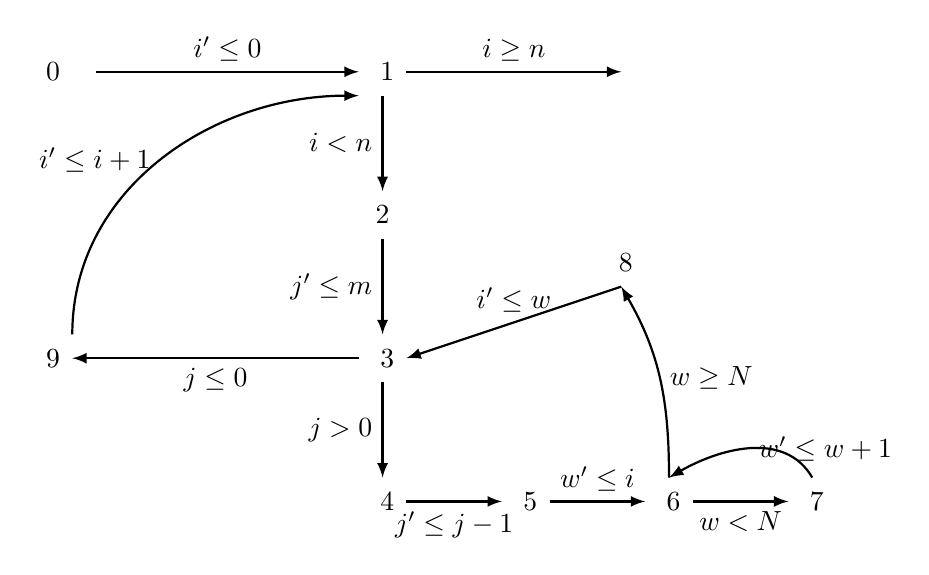
\begin{tikzpicture}[scale=\textwidth/20cm,samples=200]
\draw[] (-7, 10) circle (0pt) node{{ $0$}};
\draw[] (0, 10) circle (0pt) node{{ $1$}};
\draw[] (6, 10) circle (0pt) node {{$\lex$}};
\draw[] (0, 7) circle (0pt) node{{$2$}};
\draw[] (0, 4) circle (0pt) node{{ $3$}};
\draw[] (-7, 4) circle (0pt) node{{ $9$}};
\draw[] (0, 1) circle (0pt) node{{ $4$}};
\draw[] (3, 1) circle (0pt) node{{ $5$}};
\draw[] (6, 1) circle (0pt) node{{ $6$}};
\draw[] (9, 1) circle (0pt) node{{ $7$}};
\draw[] (5, 6) circle (0pt) node{{ $8$}};
% Counter Variables
%
% Control Flow Edges:
\draw[ thick, -latex] (-6, 10)  -- node [above] {$i' \leq 0$}(-0.5, 10);
\draw[ thick, -latex] (0, 9.5)  -- node [left] {$i < n$} (0, 7.5) ;
\draw[ thick, -latex] (0, 6.5)  -- node [left] {$j' \leq m$} (0, 4.5) ;
\draw[ thick, -latex] (0, 3.5)  -- node [left] {$j > 0$} (0, 1.5) ;
\draw[ thick, -latex] (-0.5, 4)  -- node [below] {$j \leq 0$} (-6.5, 4) ;
\draw[ thick, -latex] (-6.5, 4.5)  to  [out=90,in=180]  node [left] {$i' \leq i + 1$ }(-0.5, 9.5);
\draw[ thick, -latex] (0.5, 10)  -- node [above] {$i \geq n$}  (5, 10);
\draw[ thick, -latex] (0.5, 1)  -- node [below] {$j' \leq j - 1$}  (2.5, 1);
\draw[ thick, -latex] (3.5, 1)  -- node [above] {$w' \leq i$}  (5.5, 1);
\draw[ thick, -latex] (6.5, 1)  -- node [below] {$w < N$}  (8.5, 1);
\draw[ thick, -latex] (6, 1.5)  to [out=90,in=-60] node [right] {$w \geq N$}  (5, 5.5);
\draw[ thick, -latex] (9, 1.5)  to  [out=120,in=30] node [right] {$w' \leq w + 1$}  (6, 1.5);
\draw[ thick, -latex] (5, 5.5)  to  node [above] {$i' \leq w$ }(0.5, 4);
\end{tikzpicture}
\caption{}
  \end{centering}
  \end{subfigure}
\caption{
(a) The Example of Nested Loop with Related Iterators
  (b) The Abstract Execution Control Flow Graph}
    \label{fig:threeNestedWhile}
\end{figure}
}
\end{example}

\begin{enumerate}
  \item  \textbf{The Abstract Control Flow Graph}: Figure~\ref{fig:threeNestedWhile}(b).

  \item \textbf{Program Refinement}
  \\
  {Simple Transition Paths:}
  %  are computed as follows,
  \\
$
      \begin{array}{llll}
          \tpath_0 = (0 \to 1)
          &
          \tpath_1 = (1 \to 2 \to 3)
          &           
          \tpath_2 = (3 \to 4 \to 5 \to 6)
          &
          \tpath_3 = (6 \to 7 \to 6)
          \\
          \tpath_6 = (1 \to \lex)
          &
          \tpath_4 = (6 \to 8 \to 3)
          &
          \tpath_5 = (3 \to 9 \to 1)
      \end{array}
$
  \\
  Refined Program:
\\
$
  \rprog = \tpath_0 ; 
1: \rprepeat(\tpath_1; 3: \rprepeat(\tpath_2; 6: \rprepeat(\tpath_3); \tpath_4); \tpath_5); \tpath_6
$
\\
Let $\rprog_1 = \rprepeat(\tpath_1; 3: \rprepeat(\tpath_2; 6: \rprepeat(\tpath_3); \tpath_4); \tpath_5)$
\\
$\rprog_3 = \rprepeat(\tpath_2; 6: \rprepeat(\tpath_3); \tpath_4)$
\\
$\rprog_6 = \rprepeat(\tpath_3)$
  \item {Path Local Reachability-bound}:
\\
$\outinB(1: \rprog_1, \tpath_1) = n - N$ \quad
$\outinB(1: \rprog_1, \tpath_5) = n - N$ \quad
$\outinB(3: \rprog_3, \tpath_2) = m$ \\
$\outinB(3: \rprog_3, \tpath_4) = m$ \quad
$\outinB(6: \rprog_6, \tpath_3) = N$ \quad
%
\\
Loop Bounds:
\\
$BD(\tpath_0) = 1$
\quad
$BD(\tpath_6) = 1$
\quad
$BD( \rprepeat(\tpath_3)) = N $
\quad
$BD(\rprog_3) = m $
\quad
$BD(\rprog_1) = n - N $
%
\item Loop Reachability-bound:
\\
\highlight{
$\lpchB(1: \rprog_1, \tpath_1) = n - N$ \quad
$\lpchB(1: \rprog_1, \tpath_5) = n - N$ \quad
$\lpchB(1: \rprog_1, \tpath_2) = n$ \\ 
$\lpchB(1: \rprog_1, \tpath_4) = n$ \quad
$\lpchB(1: \rprog_1, \tpath_3) = 1$ \quad
$\lpchB(3: \rprog_3, \tpath_4) = m$ \\
$\lpchB(3: \rprog_3, \tpath_2) = m$ \quad
$\lpchB(3: \rprog_3, \tpath_3) = 1$ \quad 
$\lpchB(6: \rprog_6, \tpath_3) = N$
}
%
%
\item Path Global Reachability-bound:
\\
$\inoutB(\rprog, \tpath_1) = n - N$ \quad
$\inoutB(\rprog, \tpath_2) = n \times m$ \quad
$\inoutB(\rprog, \tpath_0) = 1$ 
\quad
$\inoutB(\rprog, \tpath_5) = n - N$ \quad
$\inoutB(\rprog, \tpath_4) = n \times m$ \quad
$\inoutB(\rprog, \tpath_6) = 1$ 
\quad
$\inoutB(\rprog, \tpath_3) = N$
%
\item The Reachability-bound:
\\
$\psRB(0) = \psRB(\lex) = 1$ \quad
$\psRB(1) = n - N + 1$ \quad
$\psRB(2) = \psRB(9) = n - N$ \quad
$\psRB(7) = N$
\\
$\psRB(3) = n - N + n \times m$ \quad
$\psRB(4) = \psRB(5) = \psRB(8) = n \times m$ \quad
$\psRB(6) = N + n \times m$ 
\end{enumerate}
\todo{step by step}
\begin{example}[While with Two Counters]
  \label{ex:twoCountersWhile}
  %
  { \small
  \begin{figure}
  \centering
  \begin{subfigure}{.4\textwidth}
    \begin{centering}
    {\small
    $
    \begin{array}{l}
      \kw{twoCountersWhile}(n, m) \triangleq \\
    \clabel{ \assign{i}{n} }^{0} ; \\
    \clabel{ \assign{j}{0} }^{1} ; \\
        \ewhile ~ \clabel{i > 0}^{2} ~ \edo ~ \\
        \qquad \Big(
          \eif(\clabel{j < m}^{3}, \\
          \qquad \qquad \clabel{\assign{j}{j + 1}}^{4}; 
          \clabel{\assign{i}{i - 1}}^{5},\\
          \qquad \qquad \clabel{\assign{j}{0}}^{6});
          \Big)
        \end{array}
        $
    }
    \caption{}
    \end{centering}
    \end{subfigure}
  \begin{subfigure}{.5\textwidth}
    \begin{centering}
  %   \todo{abstract-cfg for two round}
  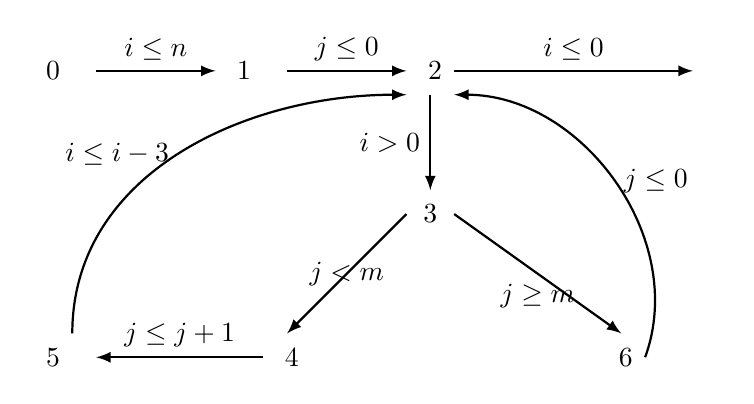
\begin{tikzpicture}[scale=\textwidth/20cm,samples=200]
  \draw[] (-8, 10) circle (0pt) node{{ $0$}};
  \draw[] (-4, 10) circle (0pt) node{{ $1$}};
  \draw[] (0, 10) circle (0pt) node{{ $2$}};
  \draw[] (0, 7) circle (0pt) node{{$3$}};
  \draw[] (-3, 4) circle (0pt) node{{ $4$}};
  \draw[] (-8, 4) circle (0pt) node{{ $5$}};
  \draw[] (4, 4) circle (0pt) node{{ $6$}};
  % Counter Variables
  \draw[] (6, 10) circle (0pt) node {\textbf{$\lex$}};
  % \draw[] (6, 4) circle (0pt) node {{ $ex$}};
  %
  % Control Flow Edges:
  \draw[ thick, -latex] (-7, 10)  -- node [above] {$i \leq n$}(-4.5, 10);
  \draw[ thick, -latex] (-3, 10)  -- node [above] {$j \leq 0$}(-0.5, 10);
  \draw[ thick, -latex] (0, 9.5)  -- node [left] {$i > 0$} (0, 7.5) ;
  \draw[ thick, -latex] (0.5, 7)  -- node [below] {$ j \geq m $}  (4, 4.5);
  \draw[ thick, -latex] (-7.5, 4.5)  to  [out=90,in=180]  node [left] {$i \leq i - 3$ }(-0.5, 9.5);
  \draw[ thick, -latex] (4.5, 4)  to  [out=70,in=0]   node [right] {$j \leq 0 $}(0.5, 9.5);
  \draw[ thick, -latex]  (-0.5, 7) -- node  {$j < m$}  (-3, 4.5) ;
  \draw[ thick, -latex]  (-3.5, 4) -- node [above] {$j \leq j + 1$}  (-7, 4) ;
  \draw[ thick, -latex] (0.5, 10)  -- node [above] {$i \leq 0$}  (5.5, 10);
  % \draw[ thick, -latex] (6, 6.5)  -- node [right] {$\top$} (6, 4.5) ;
  \end{tikzpicture}
  \caption{}
    \end{centering}
    \end{subfigure}
  \caption{
  (a) The Two Paths While Loop Example with Two Coutners
    (b) The Abstract Execution Control Flow Graph}
      \label{fig:twoCountersWhile}
  \end{figure}
  }
\end{example}

\begin{enumerate}
  \item  \textbf{The Abstract Execution Control Flow Graph} is generated in Figure~\ref{fig:twoCountersWhile}(b).

  \item \textbf{Program Rephrase and Refinement}. 
  \\
  The loop free transition paths are computed as follows,
  \[
    \begin{array}{ll}
\tpath_0 = (0 \to 1), (1 \to 2)
&
\tpath_2 = (2 \to 3), (3 \to 6), (6 \to 2)
\\
\tpath_1 = (2 \to 3), (3 \to 4), (4 \to 5), (5 \to 2)
&
\tpath_3 = (2 \to \lex)
\end{array}
\]
\textbf{Rephrased Program}:
\[
\tpath_0 ; LOOP1: \rprepeat(\rpchoose\{\tpath_1, \tpath_2 \}); \tpath_3
\]
\textbf{Refined Program}:
\[
  \tpath_0 ; LOOP1: \rpchoose\{\rprepeat_2(\rprepeat_1(\tpath_1); \tpath_2) , \rprepeat_1(\tpath_1) \}; \tpath_3
  \]
  \item \textbf{Outside-In Algorithm} : Compute Local Bound for Every program and sub programs.
  \[
    \begin{array}{l}
        LB(\tpath_0) = 1
        \\
        LB(\rprepeat_1(\tpath_1)) = m 
        \\
        LB(\rprepeat_2(\rprepeat_1(\tpath_1); \tpath_2)) = \lfloor\frac{n}{m}\rfloor
        \\
        LB(LOOP1: \rpchoose(\rprepeat_2(\cdots), \rprepeat_1(\tpath_1))) 
        = \max\{m, (m  + 1)\times \lfloor\frac{n}{m}\rfloor\}
\end{array}
\]
\item \textbf{Inside-Out Algorithm}
\begin{itemize}
  \item \textbf{Repeat Chain Set}
  \\
  $rp\mathcal{C}(LOOP1, \tpath_1) = \{\rprepeat_1(\tpath_1), \rprepeat_2(\rprepeat_1(\tpath_1); \tpath_2) \to \rprepeat_1(\tpath_1)\}$ \\
  $rp\mathcal{C}(LOOP1, \tpath_2) = \{\rprepeat_2(\cdots; \tpath_2) \to \rprepeat_1(\tpath_1)\}$ \\
  $rp\mathcal{C}(\_, \_) = \emptyset$ 
  % \\
  \item \textbf{{Local Repeat Chain Bound} }for Every Transition Path $\tpath$ on its Repeat Chain
  \\
  $rpLB(LOOP1, \tpath_1) = \max\{m, m \times \lfloor\frac{n}{m}\rfloor\}$ \\
  $rpLB(LOOP1, \tpath_2) = \lfloor\frac{n}{m}\rfloor$ 
  %
  \item \textbf{Loop Chain} Set
  \\
  $lp\mathcal{C}(\tpath_0) = \{\tpath_0\}$ \qquad
  $lp\mathcal{C}(\tpath_1) = \{LOOP1\to \tpath_1\}$ \\
  $lp\mathcal{C}(\tpath_3) = \{\tpath_3\}$ \qquad
  $lp\mathcal{C}(\tpath_2) = \{LOOP1\to \tpath_2\}$ 
  \item \textbf{Nested Loop Bound }for Every Transition Path $\tpath$ on its Loop Chain
  \\
  $rpLB(LOOP1, \tpath_1) = \max\{m, m \times \lfloor\frac{n}{m}\rfloor\}$ \quad
  $rpLB(LOOP1, \tpath_2) = \lfloor\frac{n}{m}\rfloor$  \\
  $rpLB(\bot, \tpath_0) = 1$ \quad
  $rpLB(\bot, \tpath_3) = 1$ 
  \item \textbf{Path Sensitive Reachability Bound For Every Transition Path $\tpath$ }
  \\
  $psRB(\tpath_1) = n$ \quad
  $psRB(\tpath_2) = \lfloor\frac{n}{m}\rfloor$ \quad
  $psRB(\tpath_0) = 1$ \quad
  $psRB(\tpath_3) = 1$ 
\end{itemize}
\item Step 7: Path Sensitive Reachability Bound Computation for Every Location
\\
$psRB(\{0, 1\}) = 1$ \qquad
$psRB(\{\lex\}) = 1$ \qquad
$psRB(\{6 \}) = \lfloor\frac{n}{m}\rfloor$ \\
$psRB(\{4, 5 \}) = \max\{m, m \times \lfloor\frac{n}{m}\rfloor\}$ \quad
$psRB(\{3, 2 \}) = \max\{m, m \times \lfloor\frac{n}{m}\rfloor\} + \lfloor\frac{n}{m}\rfloor + 1 $ \\
\end{enumerate}
\begin{example}[twoRounds]
    \label{ex:twoRounds}
    In this example program $\kw{towRounds(k)}$, the analyst asks in total $k+1$ queries to the mechanism in two phases.
    In the first phase, the analyst asks $k$ queries and stores the answers that are provided by the mechanism. 
    In the second phase, the analyst constructs a new query based on the results of the previous $k$ queries and sends this query to the mechanism. More specifically, we assume that, in this example, the domain $\dbdom$ 
    contains at least $k$ numeric attributes, which we index just by natural numbers. 
    The queries inside the while loop correspond to the first phase and compute an approximation of 
    the product of the empirical mean of the first $k$ attributes. 
    The query outside the loop corresponds to the second phase and computes an approximation of the empirical mean where each record is weighted by the sum of the empirical mean of the first $k$ attributes.
    %
    % Queries are of the form $q(e)$ where $e$ is an expression with a special variable $\chi$ representing a possible row. Mainly $e$ represents a function from $X$ to some domain $U$, for example $U$ could be $[-1,1]$ or $[0,1]$. This function characterizes the linear query we are interested in running. As an example, $x \leftarrow q(\chi[2])$ computes an approximation, according to the used mechanism, of the empirical mean of the second attribute, identified by $\chi[2]$. Notice that we don't materialize the mechanism but we assume that it is implicitly run when we execute the query. 
    % \jl{We use $\chi$ to abstract a possible row in the database and }
    % queries are of the form $\query(\qexpr)$, where $\qexpr$ is a special expression 
    %
    {Since statistical query computes the empirical mean of a function on rows, we use $\chi$ to abstract a possible row in the database and }
    queries are of the form $\query(\qexpr)$, where $\qexpr$ is a special expression 
    (as in our syntax in Section~\ref{sec:language})
    {
    % from $X$ to some domain $U$, 
    % for example $U$ 
      We use $U$ to denote the co-domain of queries, and it could be $[-1,1]$, $[0,1]$ or $[-R,+R]$, for some $R$ we consider.
      This function characterizes the linear query we are interested in running. 
      As an example, $x \leftarrow \query(\chi[j] \cdot \chi[k])$ computes an approximation, according to the used mechanism, of the empirical mean of the product of the $j^{th}$ attribute and $k^{th}$ attribute, identified by $\chi[j] \cdot \chi[k]$. Notice that we don't materialize the mechanism but we assume that it is implicitly run when we execute the query. } 

      The graph in Figure~\ref{fig:abscfg_twoRounds}(b). This graph is built by considering all the possible execution traces of the program in   Figure~\ref{fig:abscfg_twoRounds}(a).
      Each vertex in this graph has a superscript representing its weight, and a subscript $1$ or $0$ telling if the vertex corresponds to a query or not. We will call this subscript a query annotation. 
      For example the vertex $l^{6}:{}^{w_1}_1$, 
      % the superscript $1$ represents the weight $1$, and the subscript for the query annotation.
      has weight $w_1$, a constant function which returns $1$ for every starting state, since 
      this query at line $6$ is at most executed once regardless of the initial trace.
      The query annotation of this vertex is $1$, which  indicates that 
      $\clabel{\assign{l}{\query(\chi[k] * a)}}^6$ is a query request.
      % The assignment in the while loop, such as node $x^{3}$, 
      Another vertex, $x^{3}:{}^{w_k}_1$, appears in the while loop. 
      It has as weight a function $w_k$ that for every initial state returns the value that $k$ has in this state, since this is also the number the while loop will be iterated. 
      The node $j^{4}:{}^{w_k}_0$ has as a subscript $0$ representing a non-query assignment.
      
      
      Since the edges between two vertices represent the fact that one program variable may depend on the other,
      % the queries that are executed and the edges between two nodes represent the fact that one query may depend on the other. 
      we can define the program adaptivity with respect to a initial trace by means of a walk traversing the graph, visiting each vertex no more than its weight with respect to the initial trace, and visiting as many query nodes as possible.
      % In the walk that passes the most times of query nodes, the total visiting times of this walk on 
      % these query nodes is defined as adaptivity.
      %
      So, looking again at our example, we can see that
      % if the input variable $k$ is less than $1$ in an initial trace $\trace_1$, then it is easy to see the weight of vertex $x^3$, $w_3(\trace_1) < 1$ and we can only find a walk with one vertex $l^{6}$, according to  the definition of finite walk in Definition~\ref{def:finitewalk}. So the adaptivity for $\trace_1$, as the number of query vertices along the walk, is $1$. It is easy to understand because when $k <1$, the while loop will not be executed and only one query is asked in total. However, in reality, people want the adaptivity of this example when $k \geq 1$. With this initial trace, it is easy to see that 
      in the walk along the dotted arrows,  $l^{6} \to a^5 \to x^3 $, there are $2$ vertices with query annotation $1$ and that this number is maximal, i.e. we cannot find another walk having more than $2$ vertices with query annotation $1$, under the assumption that $k \geq 1$. So the adaptivity of the program in Figure~\ref{fig:abscfg_twoRounds}(a)  is $2$,
      % longest walk in the graph in Figure~\ref{fig:abscfg_twoRounds}(b), which we mark with a red dashed arrow, is $2$, 
      as expected.
{\small
\begin{figure} 
    \centering
    \begin{subfigure}{.2\textwidth}
    \begin{centering}
    {\small
    $
        \begin{array}{l}
              \clabel{ \assign{a}{0}}^{0} ;   
                \clabel{\assign{j}{k} }^{1} ; \\
                \ewhile ~ \clabel{j > 0}^{2} ~ \edo ~ \\
                \Big(
                 \clabel{\assign{x}{\query(\chi[j])} }^{3}  ; \\
                 \clabel{\assign{j}{j-1}}^{4} ;\\
                \clabel{\assign{a}{x + a}}^{5}       \Big);\\
                \clabel{\assign{l}{\query(\chi[k]*a)} }^{6}\\
            \end{array}
    $
    }
    \caption{}
    \end{centering}
    \end{subfigure}
      \begin{subfigure}{.35\textwidth}
      \begin{centering}
    %   \todo{abstract-cfg for two round}
    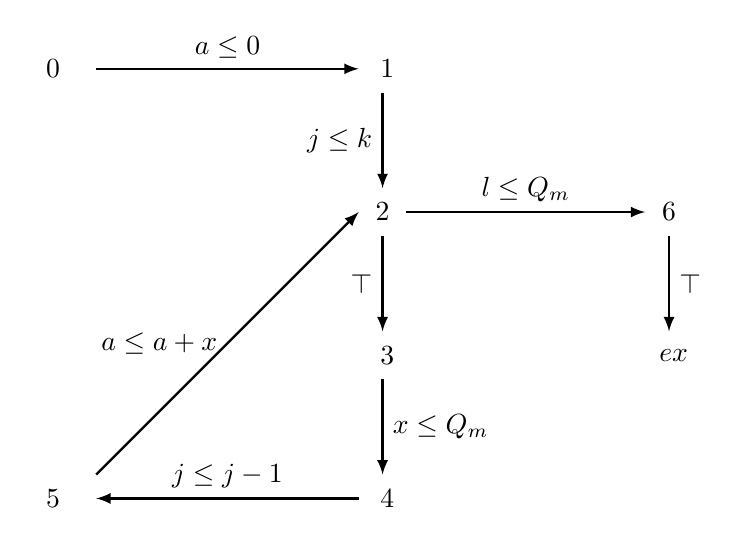
\begin{tikzpicture}[scale=\textwidth/20cm,samples=200]
    \draw[] (-7, 10) circle (0pt) node{{ $0$}};
    \draw[] (0, 10) circle (0pt) node{{ $1$}};
    \draw[] (0, 7) circle (0pt) node{\textbf{$2$}};
    \draw[] (0, 4) circle (0pt) node{{ $3$}};
    \draw[] (0, 1) circle (0pt) node{{ $4$}};
    \draw[] (-7, 1) circle (0pt) node{{ $5$}};
    % Counter Variables
    \draw[] (6, 7) circle (0pt) node {\textbf{$6$}};
    \draw[] (6, 4) circle (0pt) node {{ $ex$}};
    %
    % Control Flow Edges:
    \draw[ thick, -latex] (-6, 10)  -- node [above] {$a \leq 0$}(-0.5, 10);
    \draw[ thick, -latex] (0, 9.5)  -- node [left] {$j \leq k$} (0, 7.5) ;
    \draw[ thick, -latex] (0, 6.5)  -- node [left] {$\top$}  (0, 4.5);
    \draw[ thick, -latex] (0, 3.5)  -- node [right] {$x \leq Q_m$} (0, 1.5) ;
    \draw[ thick, -latex] (-0.5, 1)  -- node [above] {$j \leq j - 1$} (-6, 1) ;
    \draw[ thick, -latex] (-6, 1.5)  -- node [left] {$a \leq a + x$} (-0.5, 7)  ;
    \draw[ thick, -latex] (0.5, 7)  -- node [above] {$l \leq Q_m$}  (5.5, 7);
    \draw[ thick, -latex] (6, 6.5)  -- node [right] {$\top$} (6, 4.5) ;
    \end{tikzpicture}
    \caption{}
      \end{centering}
      \end{subfigure}
      \begin{subfigure}{.35\textwidth}
        \begin{centering}
      %   \todo{abstract-cfg for two round}
      \begin{tikzpicture}[scale=\textwidth/20cm,samples=200]
      \draw[] (-10, 10) circle (0pt) node{{ $0: 1$}};
      \draw[] (0, 10) circle (0pt) node{{ $1: 1$}};
      \draw[] (0, 7) circle (0pt) node{\textbf{$2: k$}};
      \draw[] (0, 4) circle (0pt) node{{ $3: k$}};
      \draw[] (0, 1) circle (0pt) node{{ $4: k$}};
      \draw[] (-10, 1) circle (0pt) node{{ $5: k$}};
      % Counter Variables
      \draw[] (6, 7) circle (0pt) node {\textbf{$6: 1$}};
      \draw[] (6, 4) circle (0pt) node {{ $ex: 1$}};
      %
      % Control Flow Edges:
    \draw[ thick, -latex] (-8, 10)  -- node [above] {$a \leq 0$}(-1.5, 10);
    \draw[ thick, -latex] (0, 9.5)  -- node [left] {$j \leq k$} (0, 7.5) ;
    \draw[ thick, -latex] (0, 6.5)  -- node [left] {$\top$}  (0, 4.5);
    \draw[ thick, -latex] (0, 3.5)  -- node [right] {$x \leq Q_m$} (0, 1.5) ;
    \draw[ thick, -latex] (-1.5, 1)  -- node [above] {$j \leq j - 1$} (-8, 1) ;
    \draw[ thick, -latex] (-8, 1.5)  -- node [left] {$a \leq a + x$} (-1.5, 7)  ;
    \draw[ thick, -latex] (1.5, 7)  -- node [above] {$l \leq Q_m$}  (4.5, 7);
    \draw[ thick, -latex] (6, 6.5)  -- node [right] {$\top$} (6, 4.5) ;
      \end{tikzpicture}
      \caption{}
        \end{centering}
        \end{subfigure}
    %       \begin{subfigure}{.3\textwidth}
    %   \begin{centering}
    %   \begin{tikzpicture}[scale=\textwidth/18cm,samples=200]
    % \draw[] (0, 10) circle (0pt) node
    % {{ $a^0: {}^1_{0}$}};
    % \draw[] (0, 7) circle (0pt) node
    % {\textbf{$x^3: {}^{k}_{1}$}};
    % \draw[] (0, 4) circle (0pt) node
    % {{ $a^5: {}^{k}_{0}$}};
    % \draw[] (0, 1) circle (0pt) node
    % {{ $l^6: {}^{1}_{1}$}};
    % % Counter Variables
    % \draw[] (5, 9) circle (0pt) node {\textbf{$j^2: {}^{1}_{0}$}};
    % \draw[] (5, 6) circle (0pt) node {{ $j^4: {}^{k}_{0}$}};
    % %
    % % Value Dependency Edges:
    % \draw[ ultra thick, -latex, densely dotted,] (0, 1.5)  -- (0, 3.5) ;
    % \draw[ ultra thick, -latex, densely dotted,] (0, 4.5)  -- (0, 6.5) ;
    % \draw[ thick, -latex] (0, 7.5)  -- (0, 9.5) ;
    % \draw[ thick, -Straight Barb] (1.5, 3.5) arc (120:-200:1);
    % \draw[ thick, -Straight Barb] (6.5, 6.5) arc (150:-150:1);
    % \draw[ thick, -latex] (5, 6.5)  -- (5, 8.5) ;
    % % Control Dependency
    % \draw[ thick,-latex] (1.5, 7)  -- (4, 9) ;
    % \draw[ thick,-latex] (1.5, 4)  -- (4, 9) ;
    % \draw[ thick,-latex] (1.5, 7)  -- (4, 6) ;
    % \draw[ thick,-latex] (1.5, 4)  -- (4, 6) ;
    % \end{tikzpicture}
    % \caption{}
    %   \end{centering}
    %   \end{subfigure}
      \vspace{-0.3cm}
      \caption{(a) The same $\kw{towRounds(k)}$ program as Figure~\ref{fig:overview-example}
      (b) The abstract control flow graph for $\kw{towRounds(k)}$  (c) The abstract control flow graph with the reachability bound for $\kw{towRounds(k)}$.}
      \vspace{-0.5cm}
      \label{fig:abscfg_twoRounds}
    \end{figure}
}
\end{example}
\input{examples_psrb/multipleRoundsOdd}
\input{examples_psrb/multipleRoundsSingle}

% \clearpage
%
% \section{Examples and Experimental Results}
% \subsection{Two Paths While Loop Example}
\begin{example}[While with Two Counters]
  \label{ex:twoCountersWhile}
  %
  { \small
  \begin{figure}
  \centering
  \begin{subfigure}{.4\textwidth}
    \begin{centering}
    {\small
    $
    \begin{array}{l}
      \kw{twoCountersWhile}(n, m) \triangleq \\
    \clabel{ \assign{i}{n} }^{0} ; \\
    \clabel{ \assign{j}{0} }^{1} ; \\
        \ewhile ~ \clabel{i > 0}^{2} ~ \edo ~ \\
        \qquad \Big(
          \eif(\clabel{j < m}^{3}, \\
          \qquad \qquad \clabel{\assign{j}{j + 1}}^{4}; 
          \clabel{\assign{i}{i - 1}}^{5},\\
          \qquad \qquad \clabel{\assign{j}{0}}^{6});
          \Big)
        \end{array}
        $
    }
    \caption{}
    \end{centering}
    \end{subfigure}
  \begin{subfigure}{.5\textwidth}
    \begin{centering}
  %   \todo{abstract-cfg for two round}
  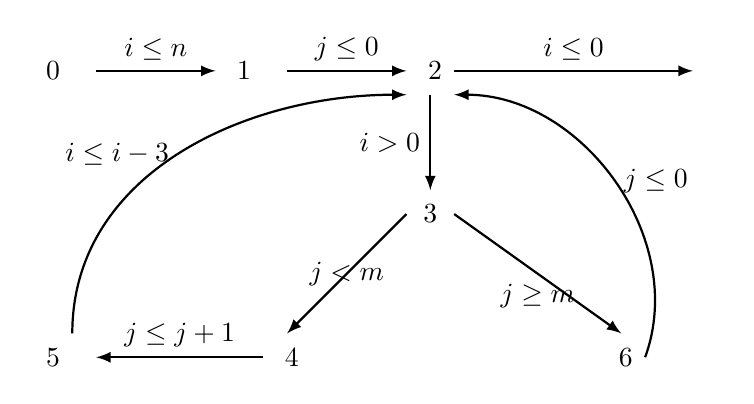
\begin{tikzpicture}[scale=\textwidth/20cm,samples=200]
  \draw[] (-8, 10) circle (0pt) node{{ $0$}};
  \draw[] (-4, 10) circle (0pt) node{{ $1$}};
  \draw[] (0, 10) circle (0pt) node{{ $2$}};
  \draw[] (0, 7) circle (0pt) node{{$3$}};
  \draw[] (-3, 4) circle (0pt) node{{ $4$}};
  \draw[] (-8, 4) circle (0pt) node{{ $5$}};
  \draw[] (4, 4) circle (0pt) node{{ $6$}};
  % Counter Variables
  \draw[] (6, 10) circle (0pt) node {\textbf{$\lex$}};
  % \draw[] (6, 4) circle (0pt) node {{ $ex$}};
  %
  % Control Flow Edges:
  \draw[ thick, -latex] (-7, 10)  -- node [above] {$i \leq n$}(-4.5, 10);
  \draw[ thick, -latex] (-3, 10)  -- node [above] {$j \leq 0$}(-0.5, 10);
  \draw[ thick, -latex] (0, 9.5)  -- node [left] {$i > 0$} (0, 7.5) ;
  \draw[ thick, -latex] (0.5, 7)  -- node [below] {$ j \geq m $}  (4, 4.5);
  \draw[ thick, -latex] (-7.5, 4.5)  to  [out=90,in=180]  node [left] {$i \leq i - 3$ }(-0.5, 9.5);
  \draw[ thick, -latex] (4.5, 4)  to  [out=70,in=0]   node [right] {$j \leq 0 $}(0.5, 9.5);
  \draw[ thick, -latex]  (-0.5, 7) -- node  {$j < m$}  (-3, 4.5) ;
  \draw[ thick, -latex]  (-3.5, 4) -- node [above] {$j \leq j + 1$}  (-7, 4) ;
  \draw[ thick, -latex] (0.5, 10)  -- node [above] {$i \leq 0$}  (5.5, 10);
  % \draw[ thick, -latex] (6, 6.5)  -- node [right] {$\top$} (6, 4.5) ;
  \end{tikzpicture}
  \caption{}
    \end{centering}
    \end{subfigure}
  \caption{
  (a) The Two Paths While Loop Example with Two Coutners
    (b) The Abstract Execution Control Flow Graph}
      \label{fig:twoCountersWhile}
  \end{figure}
  }
\end{example}

\begin{enumerate}
  \item  \textbf{The Abstract Execution Control Flow Graph} is generated in Figure~\ref{fig:twoCountersWhile}(b).

  \item \textbf{Program Rephrase and Refinement}. 
  \\
  The loop free transition paths are computed as follows,
  \[
    \begin{array}{ll}
\tpath_0 = (0 \to 1), (1 \to 2)
&
\tpath_2 = (2 \to 3), (3 \to 6), (6 \to 2)
\\
\tpath_1 = (2 \to 3), (3 \to 4), (4 \to 5), (5 \to 2)
&
\tpath_3 = (2 \to \lex)
\end{array}
\]
\textbf{Rephrased Program}:
\[
\tpath_0 ; LOOP1: \rprepeat(\rpchoose\{\tpath_1, \tpath_2 \}); \tpath_3
\]
\textbf{Refined Program}:
\[
  \tpath_0 ; LOOP1: \rpchoose\{\rprepeat_2(\rprepeat_1(\tpath_1); \tpath_2) , \rprepeat_1(\tpath_1) \}; \tpath_3
  \]
  \item \textbf{Outside-In Algorithm} : Compute Local Bound for Every program and sub programs.
  \[
    \begin{array}{l}
        LB(\tpath_0) = 1
        \\
        LB(\rprepeat_1(\tpath_1)) = m 
        \\
        LB(\rprepeat_2(\rprepeat_1(\tpath_1); \tpath_2)) = \lfloor\frac{n}{m}\rfloor
        \\
        LB(LOOP1: \rpchoose(\rprepeat_2(\cdots), \rprepeat_1(\tpath_1))) 
        = \max\{m, (m  + 1)\times \lfloor\frac{n}{m}\rfloor\}
\end{array}
\]
\item \textbf{Inside-Out Algorithm}
\begin{itemize}
  \item \textbf{Repeat Chain Set}
  \\
  $rp\mathcal{C}(LOOP1, \tpath_1) = \{\rprepeat_1(\tpath_1), \rprepeat_2(\rprepeat_1(\tpath_1); \tpath_2) \to \rprepeat_1(\tpath_1)\}$ \\
  $rp\mathcal{C}(LOOP1, \tpath_2) = \{\rprepeat_2(\cdots; \tpath_2) \to \rprepeat_1(\tpath_1)\}$ \\
  $rp\mathcal{C}(\_, \_) = \emptyset$ 
  % \\
  \item \textbf{{Local Repeat Chain Bound} }for Every Transition Path $\tpath$ on its Repeat Chain
  \\
  $rpLB(LOOP1, \tpath_1) = \max\{m, m \times \lfloor\frac{n}{m}\rfloor\}$ \\
  $rpLB(LOOP1, \tpath_2) = \lfloor\frac{n}{m}\rfloor$ 
  %
  \item \textbf{Loop Chain} Set
  \\
  $lp\mathcal{C}(\tpath_0) = \{\tpath_0\}$ \qquad
  $lp\mathcal{C}(\tpath_1) = \{LOOP1\to \tpath_1\}$ \\
  $lp\mathcal{C}(\tpath_3) = \{\tpath_3\}$ \qquad
  $lp\mathcal{C}(\tpath_2) = \{LOOP1\to \tpath_2\}$ 
  \item \textbf{Nested Loop Bound }for Every Transition Path $\tpath$ on its Loop Chain
  \\
  $rpLB(LOOP1, \tpath_1) = \max\{m, m \times \lfloor\frac{n}{m}\rfloor\}$ \quad
  $rpLB(LOOP1, \tpath_2) = \lfloor\frac{n}{m}\rfloor$  \\
  $rpLB(\bot, \tpath_0) = 1$ \quad
  $rpLB(\bot, \tpath_3) = 1$ 
  \item \textbf{Path Sensitive Reachability Bound For Every Transition Path $\tpath$ }
  \\
  $psRB(\tpath_1) = n$ \quad
  $psRB(\tpath_2) = \lfloor\frac{n}{m}\rfloor$ \quad
  $psRB(\tpath_0) = 1$ \quad
  $psRB(\tpath_3) = 1$ 
\end{itemize}
\item Step 7: Path Sensitive Reachability Bound Computation for Every Location
\\
$psRB(\{0, 1\}) = 1$ \qquad
$psRB(\{\lex\}) = 1$ \qquad
$psRB(\{6 \}) = \lfloor\frac{n}{m}\rfloor$ \\
$psRB(\{4, 5 \}) = \max\{m, m \times \lfloor\frac{n}{m}\rfloor\}$ \quad
$psRB(\{3, 2 \}) = \max\{m, m \times \lfloor\frac{n}{m}\rfloor\} + \lfloor\frac{n}{m}\rfloor + 1 $ \\
\end{enumerate}
\subsection{Three Nested While Loop with Related Iterator Example}
\begin{example}[Nested Loop with Related Iterators]
  \label{ex:threeNestedWhile}
  %
  %
  { \small
\begin{figure}
\centering
\begin{subfigure}{.4\textwidth}
  \begin{centering}
  {\footnotesize
  $
  \begin{array}{l}
      \kw{relatedNestedWhile}(n, m, N) \triangleq \\
      \clabel{ \assign{i}{0} }^{0} ; \\
          \ewhile ~ \clabel{i < n}^{1} ~ \edo ~ \\
          \qquad \Big(
           \clabel{\assign{j}{m}}^{2} ;\\
           \qquad \ewhile ~ \clabel{j > 0}^{3} ~ \edo ~ \\
           \qquad \qquad \Big(
            \clabel{\assign{j}{j-1}}^{4};
            \clabel{\assign{w}{i}}^{5};\\
            \qquad \qquad \ewhile ~ \clabel{w < N}^{6} ~ \edo ~
            \Big(
              \clabel{\assign{w}{w + 1}}^{7}
                \Big); \\
                \qquad \qquad \clabel{\assign{i}{w}}^{8}
                \Big); \\
                \qquad \clabel{\assign{i}{i+1}}^{9}
            \Big)
      \end{array}
  $
  }
  \caption{}
  \end{centering}
  \end{subfigure}
\begin{subfigure}{.5\textwidth}
  \begin{centering}
%   \todo{abstract-cfg for two round}
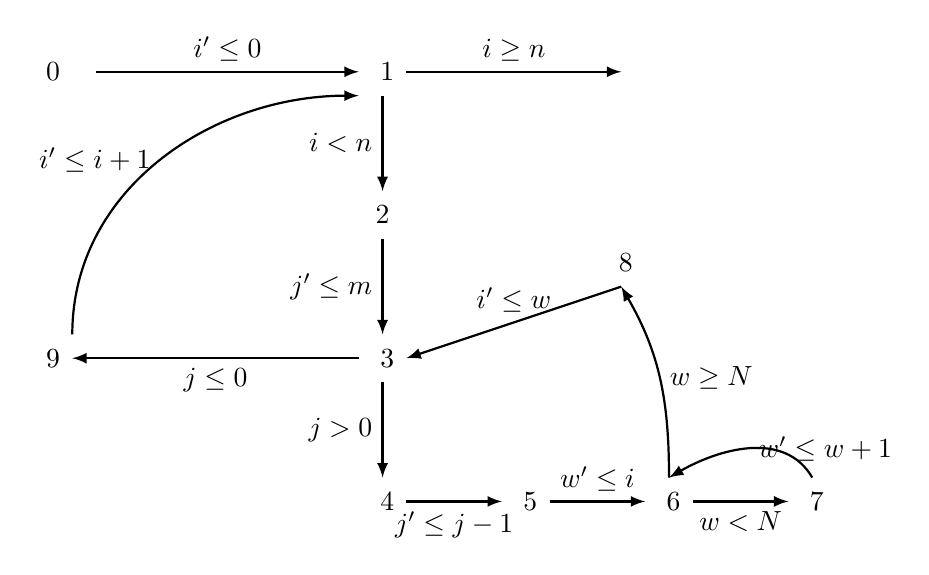
\begin{tikzpicture}[scale=\textwidth/20cm,samples=200]
\draw[] (-7, 10) circle (0pt) node{{ $0$}};
\draw[] (0, 10) circle (0pt) node{{ $1$}};
\draw[] (6, 10) circle (0pt) node {{$\lex$}};
\draw[] (0, 7) circle (0pt) node{{$2$}};
\draw[] (0, 4) circle (0pt) node{{ $3$}};
\draw[] (-7, 4) circle (0pt) node{{ $9$}};
\draw[] (0, 1) circle (0pt) node{{ $4$}};
\draw[] (3, 1) circle (0pt) node{{ $5$}};
\draw[] (6, 1) circle (0pt) node{{ $6$}};
\draw[] (9, 1) circle (0pt) node{{ $7$}};
\draw[] (5, 6) circle (0pt) node{{ $8$}};
% Counter Variables
%
% Control Flow Edges:
\draw[ thick, -latex] (-6, 10)  -- node [above] {$i' \leq 0$}(-0.5, 10);
\draw[ thick, -latex] (0, 9.5)  -- node [left] {$i < n$} (0, 7.5) ;
\draw[ thick, -latex] (0, 6.5)  -- node [left] {$j' \leq m$} (0, 4.5) ;
\draw[ thick, -latex] (0, 3.5)  -- node [left] {$j > 0$} (0, 1.5) ;
\draw[ thick, -latex] (-0.5, 4)  -- node [below] {$j \leq 0$} (-6.5, 4) ;
\draw[ thick, -latex] (-6.5, 4.5)  to  [out=90,in=180]  node [left] {$i' \leq i + 1$ }(-0.5, 9.5);
\draw[ thick, -latex] (0.5, 10)  -- node [above] {$i \geq n$}  (5, 10);
\draw[ thick, -latex] (0.5, 1)  -- node [below] {$j' \leq j - 1$}  (2.5, 1);
\draw[ thick, -latex] (3.5, 1)  -- node [above] {$w' \leq i$}  (5.5, 1);
\draw[ thick, -latex] (6.5, 1)  -- node [below] {$w < N$}  (8.5, 1);
\draw[ thick, -latex] (6, 1.5)  to [out=90,in=-60] node [right] {$w \geq N$}  (5, 5.5);
\draw[ thick, -latex] (9, 1.5)  to  [out=120,in=30] node [right] {$w' \leq w + 1$}  (6, 1.5);
\draw[ thick, -latex] (5, 5.5)  to  node [above] {$i' \leq w$ }(0.5, 4);
\end{tikzpicture}
\caption{}
  \end{centering}
  \end{subfigure}
\caption{
(a) The Example of Nested Loop with Related Iterators
  (b) The Abstract Execution Control Flow Graph}
    \label{fig:threeNestedWhile}
\end{figure}
}
\end{example}

\begin{enumerate}
  \item  \textbf{The Abstract Control Flow Graph}: Figure~\ref{fig:threeNestedWhile}(b).

  \item \textbf{Program Refinement}
  \\
  {Simple Transition Paths:}
  %  are computed as follows,
  \\
$
      \begin{array}{llll}
          \tpath_0 = (0 \to 1)
          &
          \tpath_1 = (1 \to 2 \to 3)
          &           
          \tpath_2 = (3 \to 4 \to 5 \to 6)
          &
          \tpath_3 = (6 \to 7 \to 6)
          \\
          \tpath_6 = (1 \to \lex)
          &
          \tpath_4 = (6 \to 8 \to 3)
          &
          \tpath_5 = (3 \to 9 \to 1)
      \end{array}
$
  \\
  Refined Program:
\\
$
  \rprog = \tpath_0 ; 
1: \rprepeat(\tpath_1; 3: \rprepeat(\tpath_2; 6: \rprepeat(\tpath_3); \tpath_4); \tpath_5); \tpath_6
$
\\
Let $\rprog_1 = \rprepeat(\tpath_1; 3: \rprepeat(\tpath_2; 6: \rprepeat(\tpath_3); \tpath_4); \tpath_5)$
\\
$\rprog_3 = \rprepeat(\tpath_2; 6: \rprepeat(\tpath_3); \tpath_4)$
\\
$\rprog_6 = \rprepeat(\tpath_3)$
  \item {Path Local Reachability-bound}:
\\
$\outinB(1: \rprog_1, \tpath_1) = n - N$ \quad
$\outinB(1: \rprog_1, \tpath_5) = n - N$ \quad
$\outinB(3: \rprog_3, \tpath_2) = m$ \\
$\outinB(3: \rprog_3, \tpath_4) = m$ \quad
$\outinB(6: \rprog_6, \tpath_3) = N$ \quad
%
\\
Loop Bounds:
\\
$BD(\tpath_0) = 1$
\quad
$BD(\tpath_6) = 1$
\quad
$BD( \rprepeat(\tpath_3)) = N $
\quad
$BD(\rprog_3) = m $
\quad
$BD(\rprog_1) = n - N $
%
\item Loop Reachability-bound:
\\
\highlight{
$\lpchB(1: \rprog_1, \tpath_1) = n - N$ \quad
$\lpchB(1: \rprog_1, \tpath_5) = n - N$ \quad
$\lpchB(1: \rprog_1, \tpath_2) = n$ \\ 
$\lpchB(1: \rprog_1, \tpath_4) = n$ \quad
$\lpchB(1: \rprog_1, \tpath_3) = 1$ \quad
$\lpchB(3: \rprog_3, \tpath_4) = m$ \\
$\lpchB(3: \rprog_3, \tpath_2) = m$ \quad
$\lpchB(3: \rprog_3, \tpath_3) = 1$ \quad 
$\lpchB(6: \rprog_6, \tpath_3) = N$
}
%
%
\item Path Global Reachability-bound:
\\
$\inoutB(\rprog, \tpath_1) = n - N$ \quad
$\inoutB(\rprog, \tpath_2) = n \times m$ \quad
$\inoutB(\rprog, \tpath_0) = 1$ 
\quad
$\inoutB(\rprog, \tpath_5) = n - N$ \quad
$\inoutB(\rprog, \tpath_4) = n \times m$ \quad
$\inoutB(\rprog, \tpath_6) = 1$ 
\quad
$\inoutB(\rprog, \tpath_3) = N$
%
\item The Reachability-bound:
\\
$\psRB(0) = \psRB(\lex) = 1$ \quad
$\psRB(1) = n - N + 1$ \quad
$\psRB(2) = \psRB(9) = n - N$ \quad
$\psRB(7) = N$
\\
$\psRB(3) = n - N + n \times m$ \quad
$\psRB(4) = \psRB(5) = \psRB(8) = n \times m$ \quad
$\psRB(6) = N + n \times m$ 
\end{enumerate}
\subsection{Simplified Nested Loop with Related Iterator Example}
\begin{example}[A Simplified Nested Loop with Related Iterator Example]
  \label{ex:relatedNestedWhileSim}
  %
  %
  { \small
\begin{figure}
\centering
\begin{subfigure}{.4\textwidth}
  \begin{centering}
  {\footnotesize
  $
  \begin{array}{l}
      \kw{relatedNestedWhileSim}(n, m, N) \triangleq \\
      \clabel{ \assign{i}{0} }^{0} ; \\
          \ewhile ~ \clabel{i < n}^{1} ~ \edo ~ \\
          \qquad \Big(
            \clabel{\assign{w}{i}}^{2};\\
            \qquad \ewhile ~ \clabel{w < N}^{3} ~ \edo ~
            \Big(
              \clabel{\assign{w}{w + 1}}^{4}
                \Big); \\
                \qquad \clabel{\assign{i}{w}}^{5};
                \clabel{\assign{i}{i+1}}^{6}
            \Big)
      \end{array}
  $
  }
  \caption{}
  \end{centering}
  \end{subfigure}
\begin{subfigure}{.5\textwidth}
  \begin{centering}
%   \todo{abstract-cfg for two round}
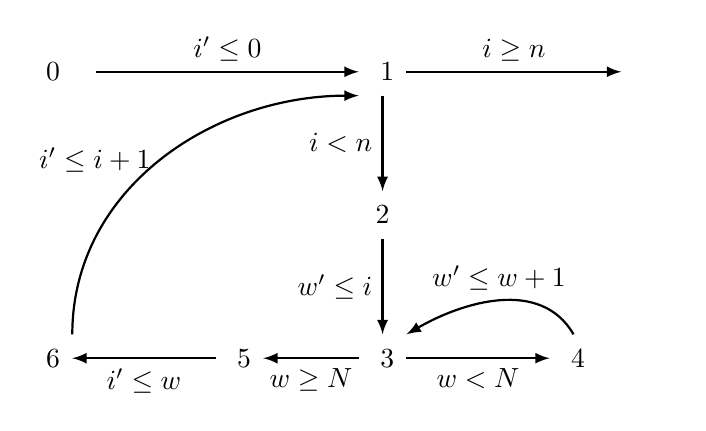
\begin{tikzpicture}[scale=\textwidth/20cm,samples=200]
\draw[] (-7, 10) circle (0pt) node{{ $0$}};
\draw[] (0, 10) circle (0pt) node{{ $1$}};
\draw[] (6, 10) circle (0pt) node {{$\lex$}};
\draw[] (0, 7) circle (0pt) node{{$2$}};
\draw[] (0, 4) circle (0pt) node{{ $3$}};
\draw[] (-7, 4) circle (0pt) node{{ $6$}};
\draw[] (-3, 4) circle (0pt) node{{ $5$}};
\draw[] (4, 4) circle (0pt) node{{ $4$}};
% Counter Variables
%
% Control Flow Edges:
\draw[ thick, -latex] (-6, 10)  -- node [above] {$i' \leq 0$}(-0.5, 10);
\draw[ thick, -latex] (0, 9.5)  -- node [left] {$i < n$} (0, 7.5) ;
\draw[ thick, -latex] (0, 6.5)  -- node [left] {$w' \leq i$} (0, 4.5) ;
\draw[ thick, -latex] (-0.5, 4)  -- node [below] {$w \geq N$} (-2.5, 4) ;
\draw[ thick, -latex] (-3.5, 4)  -- node [below] {$i' \leq w$} (-6.5, 4) ;
\draw[ thick, -latex] (-6.5, 4.5)  to  [out=90,in=180]  node [left] {$i' \leq i + 1$ }(-0.5, 9.5);
\draw[ thick, -latex] (0.5, 10)  -- node [above] {$i \geq n$}  (5, 10);
\draw[ thick, -latex] (4, 4.5)  to  [out=120,in=30] node [above] {$w' \leq w + 1$}  (0.5, 4.5);
\draw[ thick, -latex] (0.5, 4)  -- node [below] {$w < N$}  (3.5, 4);
\end{tikzpicture}
\caption{}
  \end{centering}
  \end{subfigure}
\caption{
(a) The Simplified Example of Nested Loop with Related Iterator
  (b) The Abstract Execution Control Flow Graph}
    \label{fig:relatedNestedWhileSim}
\end{figure}
}
\end{example}

\begin{enumerate}
  \item  \textbf{The Constraint Program (Abstract Control Flow Graph)} is generated in Figure~\ref{fig:threeNestedWhile}(b).

  \item \textbf{Program Refinement}
  \\
  The loop free simple transition paths are computed as follows,
  \[
      % \begin{array}{lllll}
          \tpath_0 = (0 \to 1)
          \quad
          \tpath_1 = (1 \to 2 \to 3)
          \quad           
          \tpath_2 = (3 \to 4 \to 3)
          \quad
          \tpath_3 = (3 \to 5 \to 6 \to 1)
          \quad
          \tpath_4 = (1 \to \lex)
      % \end{array}
      \]
  \textbf{Refined Program}:
  \[
  \rprog = \tpath_0 ; 1: \rprepeat(\tpath_1; 3: \rprepeat(\tpath_2); \tpath_3); \tpath_4
  \]
  \item \textbf{Outside-In Algorithm}: The \emph{OutIn} bound for the $\rprog$ and every nested repeat patterns.
  \\
$\outinB(\tpath_0) = 1$
\quad
$\outinB(3: \rprepeat(\tpath_2)) = N $
\\
$\outinB(1: \rprepeat(\tpath_1; 3: \rprepeat(\tpath_2); \tpath_3)) = n - N $
\item \textbf{Inside-Out Algorithm}
\begin{itemize}
  \item \textbf{Repeat Chain Set}
  \\
  $\rpchset(1, \tpath_1) = \{\rprepeat(\tpath_1; 3: \rprepeat(\tpath_2); \tpath_3)\}$
  \\
  $\rpchset(1, \tpath_3) = \{\rprepeat(\tpath_1; 3: \rprepeat(\tpath_2); \tpath_3)\}$
  \\
  $\rpchset(3, \tpath_2) = \{\rprepeat(\tpath_2)\}$ \quad
  $\rpchset(_, \_) = \emptyset$ 
  % \\
  \item \textbf{Repeat Chain Bound} for every simple transition path $\tpath$ through its \emph{Repeat Chain}s
  \\
  $\rpchB(1, \tpath_1) = n - N$ \quad
  $\rpchB(1, \tpath_3) = n - N$ \quad
  $\rpchB(3, \tpath_2) = N$ \quad
  $\rpchB(_, \_) = \bot $ 
  %
  \item \textbf{Loop Chain}
  \\
  $\lpch(\tpath_1) = 1\to \tpath_1$ \quad
  \highlight{$\lpch(\tpath_2) = 1 \to 3 \to \tpath_2$} \quad
  $\lpch(\tpath_3) = 1 \to \tpath_3$ \\
  $\lpch(\tpath_0) = \tpath_0$ \quad
  $\lpch(\tpath_4) = \tpath_4$
  \item \textbf{{Relative Loop Bound}} for every simple transition path $\tpath$ through its \emph{Loop Chain}
  \\
  $\rpchB(1, \tpath_1) = n - N$ \quad
  $\rpchB(1, \tpath_3) = n - N$ \quad
  \highlight{$\rpchB(1, \tpath_2) = 1$} \quad
  $\rpchB(3, \tpath_2) = N$ \quad
  $\rpchB(_, \_) = 1 $ 
  \item \textbf{Path-Sensitive Reachability-Bound} for every simple transition path $\tpath$
  \\
  $\inoutB(\tpath_1) = n - N$ \quad
  $\inoutB(\tpath_2) = N$ \quad
  $\inoutB(\tpath_0) = 1$ 
  \\
  \highlight{ $\inoutB(\tpath_3) = n - N$} \quad
  $\inoutB(\tpath_4) = 1$ 
  \end{itemize}
\item \textbf{Path Sensitive Reachability-Bound} on every program control location
\\
$\psRB(\{0, \lex\}) = 1$ \quad
$\psRB(\{1\}) = n - N + 1$ \quad
$\psRB(\{2, 5, 6\}) = n - N$ \\
\highlight{$\psRB(\{3\}) = N + 1 + n - N = n + 1$} \quad
$\psRB(\{4\}) = N$
\end{enumerate}
\subsection{Nested Loop with Iterator Reset Chain Example}
\begin{example}[Nested Loop with Variable Reset Chain]
  \label{ex:nestedWhileResetChain}
  %
  %
  { \small
\begin{figure}
\centering
\begin{subfigure}{.4\textwidth}
  \begin{centering}
  {\small
  $
  \begin{array}{l}
      \kw{nestedWhileResetChain}(n) \triangleq \\
      \clabel{ \assign{i}{n} }^{0} ; \\
      \clabel{ \assign{r}{n} }^{1} ; \\
          \ewhile ~ \clabel{i > 0}^{2} ~ \edo ~ \\
          \qquad \Big( \clabel{\assign{r}{r + 1}}^{3};\\
            \qquad  \clabel{\assign{k}{r}}^{4};\\
            \qquad \ewhile ~ \clabel{k > 0}^{5} ~ \edo ~
            \Big( \clabel{\assign{k}{k - 1}}^{6}   \Big); \\
                \qquad \clabel{\assign{r}{k}}^{7};
                \clabel{\assign{i}{i-1}}^{8}
            \Big)
      \end{array}
  $
  }
  \caption{}
  \end{centering}
  \end{subfigure}
\begin{subfigure}{.5\textwidth}
  \begin{centering}
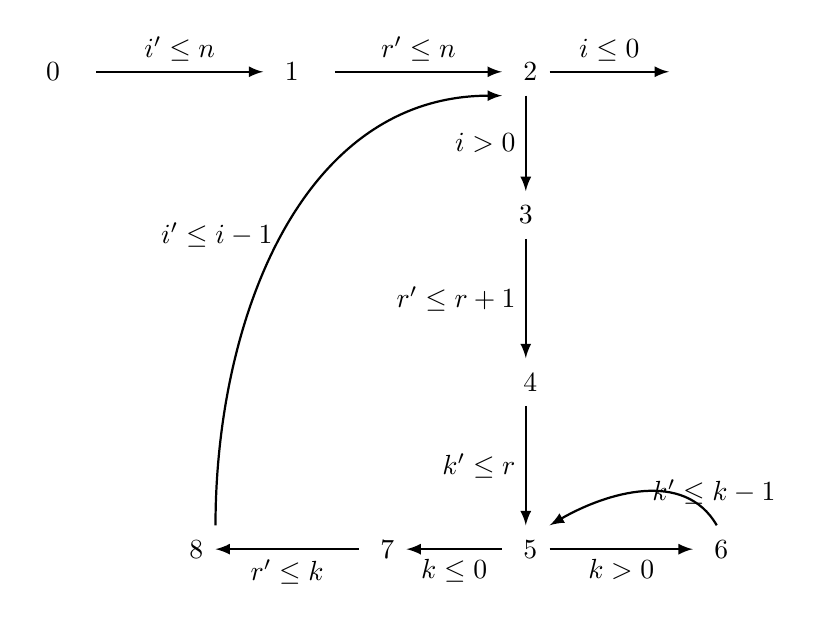
\begin{tikzpicture}[scale=\textwidth/20cm,samples=200]
\draw[] (-10, 10) circle (0pt) node{{ $0$}};
\draw[] (-5, 10) circle (0pt) node{{ $1$}};
\draw[] (0, 10) circle (0pt) node{{ $2$}};
\draw[] (4, 10) circle (0pt) node {{$\lex$}};
%
\draw[] (0, 7) circle (0pt) node{{$3$}};
\draw[] (0, 3.5) circle (0pt) node{{ $4$}};
\draw[] (0, 0) circle (0pt) node{{ $5$}};
\draw[] (4, 0) circle (0pt) node{{ $6$}};
%
\draw[] (-3, 0) circle (0pt) node{{ $7$}};
\draw[] (-7, 0) circle (0pt) node{{ $8$}};
% Counter Variables
%
% Control Flow Edges:
\draw[ thick, -latex] (-9, 10)  -- node [above] {$i' \leq n$}(-5.5, 10);
\draw[ thick, -latex] (-4, 10)  -- node [above] {$r' \leq n$}(-0.5, 10);
\draw[ thick, -latex] (0.5, 10)  -- node [above] {$i \leq 0 $}  (3, 10);
\draw[ thick, -latex] (0, 9.5)  -- node [left] {$i > 0$} (0, 7.5) ;
\draw[ thick, -latex] (0, 6.5)  -- node [left] {$r' \leq r + 1$} (0, 4) ;
\draw[ thick, -latex] (0, 3)  -- node [left] {$k' \leq r$} (0, 0.5) ;
% While Guard True, Loop Body
\draw[ thick, -latex] (0.5, 0)  -- node [below] {$k > 0$}  (3.5, 0);
\draw[ thick, -latex] (4, 0.5)  to  [out=120,in=30] node [right] {$k' \leq k - 1$}  (0.5, 0.5);
% While Guard IS FALSE, RETURN BACK TO THE PREVIOUS CONTROL POINT
\draw[ thick, -latex] (-0.5, 0)  -- node [below] {$k \leq 0$} (-2.5, 0) ;
\draw[ thick, -latex] (-3.5, 0)  -- node [below] {$r' \leq k$} (-6.5, 0) ;
\draw[ thick, -latex] (-6.5, 0.5)  to  [out=90,in=180]  node [left] {$i' \leq i - 1$ }(-0.5, 9.5);
\end{tikzpicture}
\caption{}
  \end{centering}
  \end{subfigure}
\caption{
(a) The Simplified Example of Nested Loop with Related Iterator
  (b) The Abstract Execution Control Flow Graph}
    \label{fig:nestedWhileResetChain}
\end{figure}
}
\end{example}

\begin{enumerate}
  \item  \textbf{Abstract Control Flow Graph} is generated in Figure~\ref{fig:nestedWhileResetChain}(b).

  \item \textbf{Program Refinement}
  \\
  The loop free simple transition paths:
  \[
      % \begin{array}{lllll}
          \tpath_0 = (0 \to 1 \to 2)
          \quad
          \tpath_1 = (2 \to 3 \to 4 \to 5)
          \quad           
          \tpath_2 = (5 \to 6 \to 5)
          \quad
          \tpath_3 = (5 \to 7 \to 8 \to 2)
          \quad
          \tpath_4 = (2 \to \lex)
      % \end{array}
      \]
  \textbf{Refined Program}:
  \[
  \rprog = \tpath_0 ; 2: \rprepeat(\tpath_1; 5: \rprepeat(\tpath_2); \tpath_3); \tpath_4
  \]
Let $\rprog_2 = \rprepeat(\tpath_1; 5: \rprepeat(\tpath_2); \tpath_3)$
\item {Path Local Reachability Bound}:
\\
$\outinB(\rprog, \tpath_0) = 1$ \quad
$\outinB(\rprog, \tpath_4) = 1$ \\
$\outinB(2: \rprog_2, \tpath_1) = n$ \quad
$\outinB(2: \rprog_2, \tpath_3) = n$ \\
$\outinB(5: \rprepeat(\tpath_2), \tpath_2) = n + 1$
%
\\
Loop Bounds:
\\
$BD(\tpath_0) = 1$
\quad
$BD(\tpath_4) = 1$
\quad
$BD(\rprepeat(\tpath_2)) = n + 1 $
\\
$BD(\rprepeat(\tpath_1; 5: \rprepeat(\tpath_2); \tpath_3)) = n $
%
\item Loop Reachability Bound:
\\
\highlight{
$\lpchB(2: \rprog_2, \tpath_1) = n$ \quad
$\lpchB(2: \rprog_2, \tpath_3) = n$ \quad 
$\lpchB(2: \rprog_2, \tpath_2) = \frac{(n + 1) - 0}{n}$ 
\\
$\lpchB(5: \rprepeat(\tpath_2), \tpath_2) = n + 1$ \\
$\lpchB(2: \rprog_2, \tpath_4) = 0$ \quad
$\lpchB(2: \rprog_2, \tpath_0) = 0$ \quad
$\lpchB(2: \rprog_2, \tpath_0) = 0$ \quad
}
%
%
\item Path Global Reachability Bound:
\\
$\inoutB(\rprog, \tpath_0) = 1$ \quad
$\inoutB(\rprog, \tpath_1) = n$ \quad
$\inoutB(\rprog, \tpath_2) = \frac{(n + 1)^2}{n}$ \\
$\inoutB(\rprog, \tpath_3) = n$ \quad
$\inoutB(\rprog, \tpath_4) = 1$
%
\item The Reachability Bound:
\\
$\psRB(0) = \psRB(1) = \psRB(\lex) = 1$ \quad
$\psRB(2) = n + 1$ \\
$\psRB(3) = \psRB(4) =\psRB(7) = \psRB(8) = n$ \quad \\
$\psRB(6) = \frac{(n + 1)^2}{n} $ \quad
\highlight{$\psRB(\{5\}) = n + \frac{(n + 1)^2}{n}$}
\end{enumerate}
\subsection{Two Paths Loop with Nested Loop in One Path}
\begin{example}
  [Example with Two Paths Iterating Alternatively and Nested Loop in One Path]
  \label{ex:nestedWhileOdd}
  { \small
  \begin{figure}
  \centering
  \begin{subfigure}{.4\textwidth}
    \begin{centering}
    {\small
    $
    \begin{array}{l}
      \kw{nestedWhileOdd}(k) \triangleq \\
      \clabel{ \assign{i}{k} }^{0} ; \\
          \ewhile ~ \clabel{i > 0}^{1} ~ \edo ~ \\
          \qquad \Big(
            \eif(\clabel{i \% 2 = 0 }^{2},\\
            \qquad \clabel{\assign{i}{i - 1}}^{3};
            \clabel{\assign{j}{k}}^{4}; \\
            \qquad \ewhile ~ \clabel{j > 0}^{5} ~ \edo ~
            \Big( \clabel{\assign{j}{j - 1}}^{6} \Big),\\
            \qquad \clabel{\assign{i}{i - 3}}^{7});
            \Big)
      \end{array}
    $
    }
    \caption{}
    \end{centering}
    \end{subfigure}
  \begin{subfigure}{.5\textwidth}
    \begin{centering}
  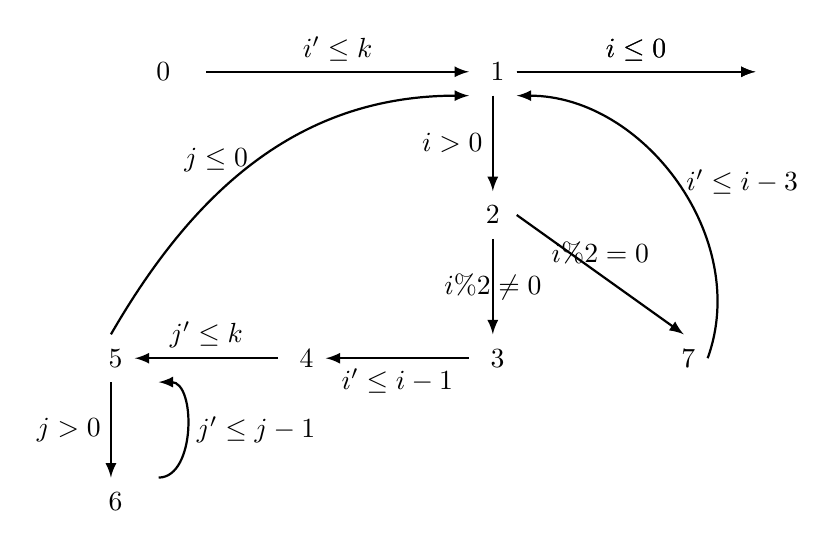
\begin{tikzpicture}[scale=\textwidth/20cm,samples=200]
  \draw[] (-7, 10) circle (0pt) node{{ $0$}};
  \draw[] (0, 10) circle (0pt) node{{ $1$}};
  \draw[] (0, 7) circle (0pt) node{\textbf{$2$}};
  \draw[] (0, 4) circle (0pt) node{{ $3$}};
  \draw[] (-4, 4) circle (0pt) node{{ $4$}};
  \draw[] (-8, 4) circle (0pt) node{{ $5$}};
  \draw[] (-8, 1) circle (0pt) node{{ $6$}};
  \draw[] (4, 4) circle (0pt) node{{ $7$}};
  % Counter Variables
  \draw[] (6, 10) circle (0pt) node {\textbf{$\lex$}};
  % \draw[] (6, 4) circle (0pt) node {{ $ex$}};
  %
  % Control Flow Edges:
  \draw[ thick, -latex] (-6, 10)  -- node [above] {$i' \leq k$}(-0.5, 10);
  \draw[ thick, -latex] (0, 9.5)  -- node [left] {$i > 0$} (0, 7.5) ;
  \draw[ thick, -latex] (0.5, 7)  -- node [above] {$ i \% 2 = 0 $}  (4, 4.5);
  \draw[ thick, -latex] (-8, 4.5)  to  [out=60,in=180]  node [left] {$j \leq 0$ }(-0.5, 9.5);
  \draw[ thick, -latex] (4.5, 4)  to  [out=70,in=0]   node [right] { $i' \leq i - 3$ }(0.5, 9.5);
  \draw[ thick, -latex]  (0, 6.5) -- node  {$i \% 2 \neq 0$}  (0, 4.5) ;
  \draw[ thick, -latex]  (-0.5, 4) -- node [below] {$i' \leq i - 1$ }  (-3.5, 4) ;
  \draw[ thick, -latex]  (-4.5, 4) -- node [above] {$j' \leq k$ }  (-7.5, 4);
  \draw[ thick, -latex] (0.5, 10)  -- node [above] {$i \leq 0$}  (5.5, 10);
  \draw[ thick, -latex] (-8, 3.5)  -- node [left] {$j > 0$}  (-8, 1.5);
  \draw[ thick, -latex] (-7, 1.5)  to  [out=0,in=0] node [right] {$j' \leq j - 1$}  (-7, 3.5);
  \draw[ thick, -latex] (0.5, 10)  -- node [above] {$i \leq 0$}  (5.5, 10);
  % \draw[ thick, -latex] (6, 6.5)  -- node [right] {$\top$} (6, 4.5) ;
  \end{tikzpicture}
  \caption{}
    \end{centering}
    \end{subfigure}
  \caption{
  (a) The program of the two paths loop with a nested Loop in one path
    (b) The Abstract Execution Control Flow Graph}
      \label{fig:nestedWhileOdd}
  \end{figure}
  }
  %
  \end{example}    
  \begin{enumerate}
    \item  \textbf{The Abstract Execution Control Flow Graph} is generated in Figure~\ref{fig:nestedWhileOdd}(b).
    \item \textbf{Program Refinement}
    \\
    The loop free simple transition paths are computed as follows,
      \\ 
    $\tpath_0 = (0 \to 1)$
      \quad
      $\tpath_1 = (1 \to 2 \to 3 \to 4 \to 5)$
      \quad
      $\tpath_2 = (5 \to 6 \to 5)$
      \quad
      $\tpath_3 = (1 \to 7 \to 2 \to 1)$
      \quad
      $\tpath_4 = (1 \to \lex)$
      \quad
      $\tpath_5 = (5 \to 1)$

  \textbf{Refined Program}:
  \[
    \tpath_0 ; \rpchoose{1: \rprepeat(\tpath_1; 5:\rprepeat(\tpath_2); \tpath_3) , 
    1: \rprepeat(\tpath_3; \tpath_1; 5:\rprepeat(\tpath_2); \tpath_5 )}; \tpath_4
    \]
    Let $\rprog_1^1 = \rprepeat(\tpath_1; 5:\rprepeat(\tpath_2); \tpath_3)$
    \\
    $\rprog_1^2 = \rprepeat(\tpath_3; \tpath_1; 5:\rprepeat(\tpath_2) ; \tpath_5 )$
    \item {Path Local Reachability-bound}:
    \\
    $\outinB(\rprog, \tpath_0) = 1$ \\
    $\outinB(\rprog, \tpath_4) = 1$ \\
    $\outinB(1: \rprog_1^1, \tpath_1) = \frac{n}{4}$ \\
    $\outinB(1: \rprog_1^1, \tpath_3) = \frac{n}{4}$ \\
    $\outinB(1: \rprog_1^1, \tpath_5) = \frac{n}{4}$ \\
    $\outinB(1: \rprog_1^2, \tpath_1) = \frac{n}{4}$ \\
    $\outinB(1: \rprog_1^2, \tpath_3) = \frac{n}{4}$ \\
    $\outinB(1: \rprog_1^2, \tpath_5) = \frac{n}{4}$ \\
    $\outinB(5: \rprepeat(\tpath_2), \tpath_2) = n$ 
    \\
    Loop Bounds:
    \\
    $BD(\tpath_0) = 1$
    \quad
    $BD(\tpath_4) = 1$
    \quad
    $BD(\rprepeat(\tpath_2)) = n $
    \quad
    $BD(\rprog_1^1) = \frac{n}{4} $
    \quad
    $BD(\rprog_1^2) = \frac{n}{4} $

    %
    \item Loop Reachability-bound:
    \\
    \highlight{
    $\lpchB(1: \rprog_1^1, \tpath_1) = \frac{n}{4}$ \quad
    $\lpchB(1: \rprog_1^1, \tpath_3) = \frac{n}{4}$ \quad 
    $\lpchB(1: \rprog_1^1, \tpath_5) = \frac{n}{4}$ \quad 
    \highlight{$\lpchB(1: \rprog_1^1, \tpath_2) = \frac{n}{4}$} \\ 
    $\lpchB(1: \rprog_1^2, \tpath_1) = \frac{n}{4}$ \quad
    $\lpchB(1: \rprog_1^2, \tpath_3) = \frac{n}{4}$ \quad 
    $\lpchB(1: \rprog_1^2, \tpath_5) = \frac{n}{4}$ \quad 
    \highlight{$\lpchB(1: \rprog_1^2, \tpath_2) = \frac{n}{4}$} \\
    $\lpchB(5: \rprepeat(\tpath_2), \tpath_2) = n$ \quad
    }
    %
    %
    \item Path Global Reachability-bound:
    \\
    $\inoutB(\rprog, \tpath_0) = 1$ \quad
    $\inoutB(\rprog, \tpath_1) = \frac{n}{4}$ \quad
    $\inoutB(\rprog, \tpath_2) = \frac{n}{4} \times n$ \\
    $\inoutB(\rprog, \tpath_3) = \frac{n}{4}$ \quad
    $\inoutB(\rprog, \tpath_5) = \frac{n}{4}$ \quad
    $\inoutB(\rprog, \tpath_4) = 1$
    %
    \item The Reachability-bound:
    \\
    $\psRB(0) = \psRB(\lex) = 1$ \quad
    $\psRB(1) = \frac{n}{2} + 1$ \quad
    $\psRB(2) = \frac{n}{2} $ \\
    $\psRB(3) = \psRB(4) = \psRB(7) = \frac{n}{4} $ \\
    \highlight{$\psRB(6) = \frac{n}{4} \times n$} \\
    $\psRB(5) =  \frac{n}{4} \times (n + 1)$
  \end{enumerate}

\subsection{Two Paths Loop with Alternative Iterations}
\begin{example}
    [While Odds Algorithm]
    \label{ex:whileOdd}
    \[
      %
      \begin{array}{l}
          \kw{whileOdd}(k) \triangleq \\
          \clabel{ \assign{i}{k} }^{0} ; \\
              \ewhile ~ \clabel{i > 0}^{1} ~ \edo ~ \\
              \qquad \Big(
                \eif(\clabel{i \% 2 == 0 }^{2}, \\
                \qquad \qquad \clabel{\assign{i}{i - 1}}^{3},\\
                \qquad \qquad \clabel{\assign{i}{i - 3}}^{4});
                \Big)
          \end{array}
      \]
    % \end{example}
    { \small
    \begin{figure}
    \centering
    %
    \begin{subfigure}{.4\textwidth}
        \begin{centering}
        \begin{tikzpicture}[scale=\textwidth/15cm,samples=200]
    % Variables Initialization
    \draw[] (5, 1) circle (0pt) node{{ $x^1: {}^1_{1}$}};
    % Variables Inside the Loop
     \draw[] (0, 7) circle (0pt) node{\highlight{ $y^5: {}^{\frac{k}{2}}_{1}$}};
     \draw[] (0, 4) circle (0pt) node{\highlight{ \boldsymbol{$p^6: {}^{\frac{k}{2}}_{1}$}}};
     \draw[] (0, 1) circle (0pt) node{{ $\mathbf{x^7: {}^{k}_{1}}$}};
     % Counter Variables
     \draw[] (5, 7) circle (0pt) node {{$j^0: {}^{1}_{0}$}};
     \draw[] (5, 4) circle (0pt) node {{ $j^3: {}^{k}_{0}$}};
     %
    % Value Dependency Edges:
             % Value Dependency Edges:
             \draw[ thick, -latex,]  (0, 3.5) -- 
             node [] {\highlight{$k $}}(0, 1.5) ;
             \draw[ thick, -Straight Barb] (6.5, 4.5) arc (150:-150:1);
             \draw[](7, 4) node [] {\highlight{$k  $}};
             \draw[ thick, -latex] (5, 4.5)  -- 
             node [right] {\highlight{$k$}}(5, 6.5) ;
             % Value Dependency Edges on Initial Values:
             \draw[ thick, -latex,] (1.5, 1)  -- 
             node [above] {\highlight{$k$}}(4, 1) ;
             %
            \draw[ ultra thick, -latex, densely dotted,] (-0.6, 1.5)  to  [out=-220,in=220]  
            node [left] {\highlight{$k $}}(-0.5, 6.5);
            \draw[ ultra thick, -latex, densely dotted,]  (0.5, 6.5) to  [out=-30,in=30] 
            node [above] {\highlight{$k $}}(0.6, 1.6) ;
             % Control Dependency
            \draw[ thick,-latex] (1.5, 7)  -- 
            node [above] {\highlight{$k$}}(4, 6) ;
            \draw[ thick,-latex] (1.5, 4)  -- 
            node [above] {\highlight{$k$}}(4, 6) ;
             \draw[ thick,-latex] (1.5, 1)  -- 
             node [below] {\highlight{$k $}}(4, 6) ;
    
    \end{tikzpicture}
    \caption{}
    \end{centering}
    \end{subfigure}
    %
            \begin{subfigure}{.5\textwidth}
                \begin{centering}
                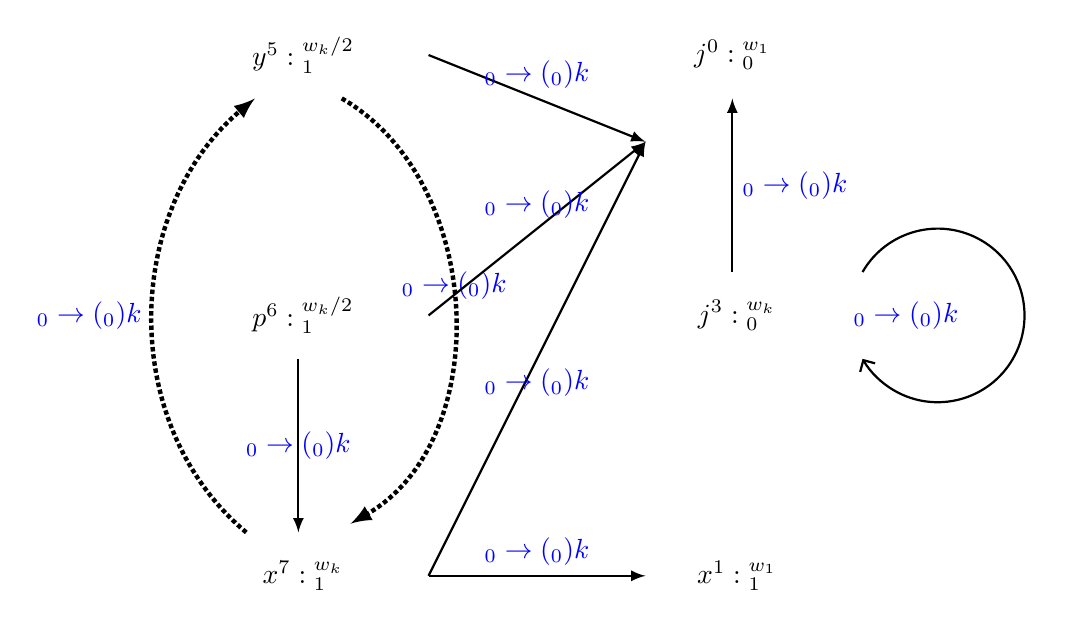
\begin{tikzpicture}[scale=\textwidth/11cm,samples=200]
            % Variables Initialization
             \draw[] (5, 1) circle (0pt) node{{ $x^1: {}^{w_1}_{1}$}};
            % Variables Inside the Loop
             \draw[] (0, 7) circle (0pt) node{{ $y^5: {}^{w_k/2}_{1}$}};
             \draw[] (0, 4) circle (0pt) node{{ $p^6: {}^{w_k/2}_{1}$}};
             \draw[] (0, 1) circle (0pt) node{{ $x^7: {}^{w_k}_{1}$}};
             % Counter Variables
             \draw[] (5, 7) circle (0pt) node {{$j^0: {}^{w_1}_{0}$}};
             \draw[] (5, 4) circle (0pt) node {{ $j^3: {}^{w_k}_{0}$}};
             %
             % Value Dependency Edges:
             \draw[ thick, -latex,]  (0, 3.5) -- 
             node [] {\highlight{$\trace_0 \to \env(\trace_0) k $}}(0, 1.5) ;
             \draw[ thick, -Straight Barb] (6.5, 4.5) arc (150:-150:1);
             \draw[](7, 4) node [] {\highlight{$\trace_0 \to \env(\trace_0) k  $}};
             \draw[ thick, -latex] (5, 4.5)  -- 
             node [right] {\highlight{$\trace_0 \to \env(\trace_0) k $}}(5, 6.5) ;
             % Value Dependency Edges on Initial Values:
             \draw[ thick, -latex,] (1.5, 1)  -- 
             node [above] {\highlight{$\trace_0 \to \env(\trace_0) k $}}(4, 1) ;
             %
            \draw[ ultra thick, -latex, densely dotted,] (-0.6, 1.5)  to  [out=-220,in=220]  
            node [left] {\highlight{$\trace_0 \to \env(\trace_0) k $}}(-0.5, 6.5);
            \draw[ ultra thick, -latex, densely dotted,]  (0.5, 6.5) to  [out=-30,in=30] 
            node [above] {\highlight{$\trace_0 \to \env(\trace_0) k $}}(0.6, 1.6) ;
             % Control Dependency
            \draw[ thick,-latex] (1.5, 7)  -- 
            node [above] {\highlight{$\trace_0 \to \env(\trace_0) k $}}(4, 6) ;
            \draw[ thick,-latex] (1.5, 4)  -- 
            node [above] {\highlight{$\trace_0 \to \env(\trace_0) k $}}(4, 6) ;
             \draw[ thick,-latex] (1.5, 1)  -- 
             node [below] {\highlight{$\trace_0 \to \env(\trace_0) k $}}(4, 6) ;
             \end{tikzpicture}
             \caption{}
                \end{centering}
                \end{subfigure}
    \caption{
    (a) The multiple rounds odd example 
    (b) The program-based dependency graph from $\THESYSTEM$
    (c) The execution-based dependency graph.}
        \label{fig:overappr_example}
    \end{figure}
    }
    %
    \end{example}    
    \begin{enumerate}
      \item Step 1: Abstract Transition Graph:
    
    \item Step 2: Path Insensitive Transition Bound Computation
    
    \item Step 3: Program Rephrase through Path Collection on Abstract CFG
    \\
    $\tpath_0 = (0, 1)$
    \\
    $\tpath_1 = (1 \to 2), (2 \to 3), (3 \to 1)$
    \\
    $\tpath_2 = (1 \to 2), (2 \to 4), (4 \to 1)$
    \\
    $\tpath_3 = (1 \to \lex)$
    \\
    Rephrased Program
    \[
    \tpath_0 ; LOOP1: \rprepeat(\rpchoose\{\tpath_1, \tpath_2 \}); \tpath_3
    \]
    \item Step 4: While Loop Refinement:
    \[
      \tpath_0 ; LOOP1: \rpchoose\{\rprepeat_3(\rprepeat_1(\tpath_1); \tpath_2) , \rprepeat_4(\rprepeat_2(\tpath_2); \tpath_1) \}; \tpath_3
      \]
    \item Step 5: Outside-In Algorithm
    \\
    $LB(\tpath_0) = 1$
    \\
    $LB(\tpath_3) = 1$
    \\
    $LB(\rprepeat_1(\tpath_1)) = 1 $
    \\
    $LB(\rprepeat_3(\rprepeat_1(\tpath_1); \tpath_2)) = \frac{n}{4} $
    \\
    $LB(\rprepeat_2(\tpath_2)) = 1 $
    \\
    $LB(\rprepeat_4(\rprepeat_2(\tpath_2); \tpath_1)) = \frac{n}{4} $
    % \\
    % $LB(LOOP1: \rpchoose(\rprepeat_2(\cdots), \rprepeat_1(\tpath_1))) 
    % = \max\{m, \frac{n}{m}\} $
    % \\
    \item Step 6: Inside-Out Algorithm
    \begin{itemize}
      \item \textbf{Repeat Chain Set}
      \\
      $rp\mathcal{C}(LOOP1, \tpath_1) = \{\rprepeat_4(\cdots, \tpath_1), \rprepeat_3(\rprepeat_1(\tpath_1); \tpath_2) \to \rprepeat_1(\tpath_1)\}$ \\
      $rp\mathcal{C}(LOOP1, \tpath_2) = \{\rprepeat_3(\cdots, \tpath_2), \rprepeat_4(\rprepeat_2(\tpath_2); \tpath_1) \to \rprepeat_2(\tpath_2)\}$ \\
      $rp\mathcal{C}(\_, \_) = \emptyset$ 
      % \\
      \item \textbf{{Local Repeat Chain Bound} for Every Transition Path $\tpath$ on its Repeat Chain}
      $rpLB(LOOP1, \tpath_1) = \frac{n}{4}$ \\
      $rpLB(LOOP1, \tpath_2) = \frac{n}{4}$ 
      %
      \item \textbf{Loop Chain}
      \\
      $lp\mathcal{C}(\tpath_1) = \{LOOP1\to \tpath_1\}$ \\
      $lp\mathcal{C}(\tpath_2) = \{LOOP1\to \tpath_2\}$ \\
      $lp\mathcal{C}(\tpath_0) = \{\tpath_0\}$ \\
      $lp\mathcal{C}(\tpath_3) = \{\tpath_3\}$ 
      \item \textbf{Nested Loop Bound for Every Transition Path $\tpath$ on its Loop Chain}
      \\
      $rpLB(LOOP1, \tpath_1) = \frac{n}{4}$ \\
      $rpLB(LOOP1, \tpath_2) = \frac{n}{4}$  \\
      $rpLB(\bot, \tpath_0) = 1$ \\
      $rpLB(\bot, \tpath_3) = 1$ 
      \item \textbf{Path Sensitive Reachability Bound For Every Transition Path $\tpath$ }
      \\
      $psRB(\tpath_1) = \frac{n}{4}$ \\
      $psRB(\tpath_2) = \frac{n}{4}$ \\
      $psRB(\tpath_0) = 1$ \\
      $psRB(\tpath_3) = 1$ 
    \end{itemize}
    \item Step 7: Path Sensitive Reachability Bound Computation for Every Location
    \\
    $psRB(\{0, 1\}) = 1$ \\
    $psRB(\{2, 3, 1 \}) = \frac{n}{4}$ \\
    $psRB(\{2, 4, 1\}) = \frac{n}{4}$ \\
    $psRB(\{\lex\}) = 1$ 
    \end{enumerate}



%
\clearpage
\appendix
\addcontentsline{toc}{section}{Appendices}
\section*{Appendices}
% \section{Language and Trace-based Operational Semantics}
\label{apdx:language}
\input{language-appendix}
\clearpage

\section{Reset Graph Based Ranking Function Estimation}
\label{apdx:alg-resetgraph}
\subsection{Reset Graph}
We  compute the reset graph $\resetG(c)$ and the reset chain, $\resetchain(c, x) \in \mathcal{P}(\mathcal{P}(\absevent))$ for every rank $x$.
  The $\resetchain(c, x)$ for every rank $x$ contains all the paths in $\resetG(c)$ that are end at $x$.
  The computation of $\resetG(c)$ and $\resetchain(c, x)$ follows the Definition~20 in~\cite{SinnZV17}.
  \[\resetG(c) = (\resetV(c), \resetE(c))\]
  \[\resetE(c) = \left\{ (x, \absevent, y) ~\vert~ \absevent \in \reset(c, x) \land \absevent = (l, x' \leq y + c, l') \right\} \]
  \[\resetV(c) = \left\{ x ~\vert~ (x, \_, \_) \in \resetE(c) \lor (\_, \_, x) \in \resetE(c) \right\} \]
  In a variable $x$'s reset chain set, $\resetchain(c, x)$, in each chain $(e_0, \ldots, e_m) \in \resetchain(c, x)$
  a variable $x_i$ is reset by another variable $x_{i + 1}$ on edge $e_{i}$
  and $x_{i + 1}$ is reset on edge $e_{i + 1}$ recursively
  for every $i = 0, \ldots, m - 1$.
  $x$ is reset on the first edge $e_0$ of every sequence in $\resetchain(c, x)$.
  {Each edge $e_i$ in a sequence $(e_0, \ldots, e_m) \in \resetchain(c, x)$
  resets a variable $x_i$ by another variable $x_{i + 1}$ such that $x_{i + 1}$
  is reset on edge $e_{i + 1}$ recursively. The first edge $e_0$ of each sequence resets the variable $x$.}
  % 
  % \subsection{Assigning The Ranking Function to An Edge}
  % For each edge in the transition graph $\absG(c)$ of a program $c$,
  % this step assigns the variable that decreases on this edge as the ranking function of this edge.
  % This step adopts the local bound computation method in Section 4 of~\cite{SinnZV17} to assign the local bound to each edge,
  % formally as follows.
  % \begin{defn}[Ranking Function Generatation]
  % \label{def:ranking_gen}
  % For every edge $\absevent$ in the transition graph $\absG(c)$ of a program $c$,
  % its \emph{ranking function/local bound}, $\locbound(\absevent, c)$
  % is the variable that decreases on this edge, computed as follows,
  % %
  % \[ 
  % \begin{array}{ll}
  %   \locbound(\absevent, c) \triangleq 1 
  %   & \absevent \notin SCC(\absG(c))
  %   \\
  %   \locbound(\absevent, c) \triangleq x
  %   & \absevent \in SCC(\absG(c)) \land \absevent \in \dec(c, x) \land  \absevent = (\_, \_ , x' \leq x - v) \\
  %   \locbound(\absevent, c) \triangleq x
  %   & \absevent \in SCC(\absG(c)) \land 
  %   \absevent  \notin \bigcup_{x \in \vardom} \dec(c, x)
  %   \land \absevent \notin SCC(\absG(c) \setminus \dec(c, x))\\
  %   \locbound(\absevent, c) \triangleq \infty
  %   & o.w..
  % \end{array}
  % \]
  % $SCC(\absG(c))$ is the set of all the strong connected components of $\absG(c)$.
  % \end{defn}
  %   The first case is straightforward. 
  %   For the label $l$ which is not in any while loop, 
  %   the labeled command with the label $l$ will be 
  %   evaluated at most once. 
  %   The second and third cases are guaranteed by the \emph{Discussion on Soundness} in Section 4 in~\cite{SinnZV17}.
  %   The soundness is formalized in Lemma~\ref{lem:local_bound_sound} with proof in Appendix~\ref{apdx:pathinsensitive_rb_soundness}.
  % %
  \subsection{Reset Graph Based Ranking Function Estimation}
  This step estimates the upper bound, $\varinvar(x, c) \in \scexpr(c)$
  on the maximum value for each ranking function  $x \in  \vardom \cup \scvar(c)$.
  \\
  For a program $c$, the \emph{ranking function bound},
  $\varinvar(\locbound(\absevent, c), c)$ is 
  the bound on the maximum value of the ranking function  
  assigned to the edge $\absevent \in \absE(c)$, formally in Definition~\ref{def:ranking_bound}.
  \\
  In order to estimate the maximum value of $\locbound(\absevent, c)$ assigned to edge $\absevent \in \absE(c)$,
  the bound on the iteration times of each corresponding edge, $\absclr(\absevent, c)$ 
  is computed interactively in a path-insensitive manner.
  \begin{defn}[Ranking Function Estimation]
    % \label{def:ranking_bound}
  For a program $c$ and an edge $\absevent \in \absE(c)$,
  the \emph{ranking function bound}, 
  $\varinvar(\locbound(\absevent, c), c)$ for the ranking function $x = \locbound(\absevent, c)$
  of this edge
  is computed as follows,
    \[ 
  \begin{array}{lll}
    \varinvar(x, c) & \triangleq x & x \in \scvar(c) \\
    \varinvar(x, c) & \triangleq \incrs(x, c) + \max\left\{\varinvar(y, c) + v ~\mid~ (l, x' \leq y + v, l') \in \reset(c, x) \right\} & x \notin \scvar(c)
  \end{array}
  \]
  %
  where $\incrs(x, c) \triangleq \sum\limits_{\absevent \in \inc(c, x)}\{\absclr(\absevent, c) \times v ~\mid~ \absevent = (l, x' \leq x + v, l')\}$
  The path-insensitive bound, $\absclr(\absevent, c) \in \scexpr(c)$  on the execution times of the transition $\absevent$, is interactively computed as well as below,
\[ 
\begin{array}{lll}
  \absclr(\absevent, c) 
  & \triangleq \varinvar(\locbound(\absevent, c), c)  &  \\
  & \quad \text{if} ~ \locbound(\absevent, c) \in \scvar(c) & \\
  \absclr(\absevent, c) 
  & \triangleq
    \sum \left\{ \incrs(y, c) | ch \in \resetchain(x, c) \land y \in ch \right\} & \\
    & \quad + 
  \sum\limits_{ch \in \resetchain(x, c)}
  \min \left\{\absclr(\absevent', c) ~\mid~ \absevent' \in ch\right\} \times 
  \big(\varinvar(in(ch), c) 
  + \sum\limits_{(\_, (\_, x' \leq y + v, \_), \_) \in ch} v \big) & \\
  &  \quad \text{if} ~\locbound(\absevent, c) = x \land x \notin \scvar(c) & ,
\end{array}
  \]
 where $in(ch)$ is the first vertex of the reset chain $ch$.
\end{defn}
  %
We also have the soundness of this path-insensitive transition bound. For a program $c$ and an edge $\absevent \in \absE(c)$,
$\absclr(\absevent)$ is a sound upper bound
on the execution times of this transition by paper~\cite{SinnZV17}, formally below in Theorem~\ref{thm:pathinsensitive_rb_soundness} with proof in Appendix~\ref{apdx:pathinsensitive_rb_soundness}.
%
\begin{thm}[Soundness of the Path-insensitive Transition Bound]
  \label{thm:pathinsensitive_rb_soundness}
For each program ${c}$ and an edge $\absevent = (l, \_, \_) \in \absG(c)$, if $l$ is the label of an assignment command,
%  label $l \in \lvar(c)$,
then its \emph{path-insensitive transition bound} $\absclr(\absevent, c)$ 
 is a sound upper bound on 
the execution times of this assignment command in $c$.
  \[
    \begin{array}{l}
      \forall \trace_0 \in \ftdom_0(c), \trace \in \tdom, c \in \cdom, l, l' \in \lvar(c) \st
      \Big( \config{c, \trace_0} \rightarrow^{*} \config{\clabel{\eskip}^{l'}, \trace_0 \tracecat \trace} 
        \lor  \config{c, \trace_0} \uparrow^{\infty} \trace_0 \tracecat \trace \Big)
       \\ \qquad \qquad
       \implies
       \exists \absevent = (\_, l, \_) \in \absflow(c) \land
      \counter(\trace, l) \leq \econfig{\absclr(\absevent, c)}(\trace_0)
    \end{array}
  \]
\end{thm}

\clearpage

\section{Program Rewriting Algorithm}
\label{apdx:alg-rewrite}
{
% \vspace{-0.5cm}
\begin{algorithm}
\caption{Program Rewriting $\kw{Rewrite}$}
\label{alg:alg-refine_rewrite}
\begin{algorithmic}[1]
  \REQUIRE program $c$ and all \emph{simple transition path}s, $\tpath_1, \ldots, \tpath_n \in \paths(\absG(c))$.
  % \STATE collects all $c$'s \emph{simple transition path}s from $\absG(c)$, $\tpath_1, \ldots, \tpath_n \in \paths(\absG(c))$.
  \STATE \textbf{init}: candidate set $W = \{c_1, \ldots, c_n\}$, where $c_i = \tpath_i$ and $i = 1, \ldots, n$
  \STATE \textbf{while} $W.size()> 1$:
  \STATE \quad 
  for all $c_i \in W \land c_i.start = c_j.start \land c_i.end = c_j.end, i, j = 1, \ldots, n$.
  \\ \quad create $c' = \rpchoose{c_1, \ldots, c_m}$, \qquad  $W.add(c')$ \qquad $W.remove(c_1, \ldots, c_m)$
  \STATE
  \quad for all $c_i \in W \land c.start = c.end \land c.start \in \loopl(c)$
  \\ \quad create $c' = \rprepeat(c)$, \qquad $W.add(c')$, \qquad $W.remove(c)$
  \STATE \quad for all $c_1, c_2 \in W \land c_1.end = c_2.start$
  \\
  \quad create $c' = c_1; c_2$, \quad $W.add(c')$ \qquad $W.remove(c_1, c_2)$
  % \STATE \textbf{Endwhile}
  \RETURN $W[0]$.
\end{algorithmic}
\end{algorithm}
% \vspace{-0.5cm}
}%
Line-1, we initialize each candidate $c_i$ with a \emph{simple transition path} $\tpath_i$. New candidates generated in Line-3, 4 and 5 correspond to the if,
while and sequence statement in paper~\cite{GulwaniJK09} respectively.
The Line-3:5 are recursively updating the candidate set $W$ until $W$ is stabilized.
\begin{itemize}
  \item
  Line-4: for all the candidates $c_1, \ldots, c_m$ having the same starting and ending vertices, rewrite them into if statement as~\cite{GulwaniJK09}.
  \item
  Line-5: for every candidate $c'$, if it starts and ends with the same vertex, rewrite it into while loop statement as~\cite{GulwaniJK09}.
  \item
  Line-6: for every two candidates $c_1, c_2$, if $c_1$ ends with the same vertex as $c_2$'s starting label, rewrite them into sequence statement as~\cite{GulwaniJK09}.
\end{itemize}

\clearpage


\section{Performance Evaluation}
\label{apdx:eval-performance}
As in Tab.~\ref{tb:performance-eval}, our tool suffers the efficiency problem because of the possible non-terminating in REFINE algorithm and the ranking function estimating algorithm.
Also, since the implementation consists of the 
program abstraction in OCaml and the program refinement, ranking function estimation and the path-sensitive reachability-bound algorithm in Python.
The inter-procedures calls between the functions in different languages also reduce the efficiency to a large scale.


\begin{table}[H]
    \caption{The Performance Evaluation of {\THESYSTEM}}
    \label{tb:performance-eval}
    \centering
        {\footnotesize
        \begin{tabular}{ >{\small}c | c | c | c | c | c | c | c | c | c }
            \multirow{2}{*}{Benchmark} & \multirow{2}{*}{\# P}  & \multirow{2}{*}{M.P.L \#} & Nested  & \multirow{2}{*}{Bounded} & {Success} & \multirow{2}{*}{Failed} & Time  & Total\\
             &  &  & Loop \# & & Rate &  & Outs &   Runtime \\
            \hline
                {Loopus} & {110}  & 53  & 52  & 98 & 89.1\% & 11 & 7 & 7min42sec \\
                \hline
                Loopus-C & 23  & 20 & 20 & {20} & {86\%}  & 2 & 3 & {12min39sec} \\
                \hline
                {Icra} & 118 & 111 & 21 & 107 & 90.1\% & 11 & 1 & {4min48sec} \\
                \hline
                Tianhan & 37 & 2 & 3 & 37 & 100.0\% & 1 & 0 & 1min03sec \\
                \hline
            \end{tabular}    
        }
    \end{table}

\clearpage

\section{Proofs of Lemmas in Language Model}
\label{apdx:lem_language}
\begin{lem}[Uniqueness of the Program Labels]
  For every program $c \in \cdom$ and every two labels such that
  $i, j \in \lvar(c)$, then $i \neq j$.
  \[
    \forall c \in \cdom, i, j \in \ldom \st i, j \in \lvar(c)\implies i \neq j.
    \]
\end{lem}
  \begin{proof}
    The proof is trivially by induction on program $c$.
  \end{proof}
  \begin{lem}[Trace Non-Decreasing]
    % \label{lem:tracenondec}
    For any program $c \in \cdom$ and initial trace $\trace_0 \in \ftdom_0(c)$,
    if there exists $\trace \in \tdom$ and $c' \in \cdom $ such that $\config{c, \trace_0} \rightarrow^{*} \config{c', \trace} $ or 
    $\config{c, \trace_0} \rightarrow^{\infty} \config{c', \trace}$  
    then there exists a trace $\trace' \in \tdom$ such that $\trace_0 \tracecat \trace' = \trace$ formally as follows.
    %
    \[
      \begin{array}{l}
      \forall \trace_0 \in \ftdom_0(c), \trace \in \tdom, c, c' \in \cdom \st
      \Big( \config{c, \trace_0} \rightarrow^{*} \config{c', \trace} 
      \lor  \config{c, \trace_0} \rightarrow^{\infty} \config{c', \trace} \Big)
      \\ \quad
      \implies \exists \trace' \in \tdom \st \trace_0 \tracecat \trace' = \trace 
      \end{array}
      \]
      \end{lem}
    \begin{proof}
      Taking an arbitrary initial trace $\trace_0 \in \ftdom_0(c)$, by induction on program $c$, we have the following cases.
      \caseL{$c = [\assign{x}{\expr}]^{l}$}
      By the evaluation rule $\rname{assn}$, we have
      $
      {
      \config{\clabel{\assign{{x}}{\aexpr}}^{l},  \trace_0 } 
      \xrightarrow{} 
      \config{\clabel{\eskip}^{l}, \trace_0 :: ({x}, l, v)}
      }$, for some $v \in \mathbb{N}$.
      \\
      Let $\trace = \trace_0 ::({x}, l, v)$ and $\trace' =  [({x}, l, v) ]$,
      then we have $\trace_0 \tracecat \trace' = \trace$ and this case is proved.
      \caseL{$c = c_{1};c_{2}$}
      By the first rule applied to $c$ in operational semantics, there are two cases as follows.
      \subcaseL{$\rname{seq1}$}
      If the first rule applied to $c$ is $\rname{seq1}$, we have
      \[
        \inferrule
        {
        \config{{c_1, \trace_0}}
        \xrightarrow{}
        \config{{c_1',  \trace_1}}
        }
        {
        \config{{c_1; c_2, \trace_0}} 
        \xrightarrow{} 
        \config{{c_1'; c_2, \trace_1}}
        }
      \]
      By induction hypothesis on $c_1$, we know 
      \[
        \exists \trace_1' \in \tdom \st \trace_0 \tracecat \trace_1' = \trace_1
      \]
      Let $\trace = \trace_1$ and $\trace' =  \trace_1'$,
      then we have $\trace_0 \tracecat \trace' = \trace$ and this case is proved.
      \subcaseL{$\rname{seq2}$}
      If the first rule applied to $c$ is $\rname{seq2}$, we have
      \[
        \inferrule
        {
        \config{{c_2, \trace_0}}
        \xrightarrow{}
        \config{{c_2',  \trace_2}}
        }
        {
        \config{{\clabel{\eskip}^l; c_2, \trace_0}} 
        \xrightarrow{} 
        \config{{c_2, \trace_2}}
        }
      \]
      By induction hypothesis on $c_2$, we know 
      \[
        \exists \trace_2' \in \tdom \st \trace_0 \tracecat \trace_2' = \trace_2
      \]
      Let $\trace = \trace_2$ and $\trace' =  \trace_2'$,
      then we have $\trace_0 \tracecat \trace' = \trace$ and this case is proved.
      \caseL{$\ewhile \clabel{b}^{l_w} \edo (c_w)$}
      By the first rule applied to $c$ in operational semantics, there are two cases as follows.
      \subcaseL{$\textbf{while-t}$}
      If the first rule applied to $c$ is $\rname{while-t}$, we have
      \[
        \config{{\ewhile \clabel{b}^{l_w} \edo c_w, \trace_0}}
        \xrightarrow{} 
        \config{{
        c_w; \ewhile \clabel{b}^{l_w} \edo c_w,
        \trace_0 :: (b, l_w, \etrue)}}.
      \]
      Let $\trace = \trace_0 ::(b, l_w, \etrue)$ and $\trace' =  [(b, l_w, \etrue)]$,
      then we have $\trace_0 \tracecat \trace' = \trace$ and this case is proved.
      %   \\
      %   Let $\trace_w' \in \tdom$ be the trace satisfying following execution:
      %   \\
      %   $
      %   \config{{
      %   c_w,
      %   \trace :: (b, l_w, \etrue, \bullet)}}
      %   \xrightarrow{*} 
      %   \config{{
      %   \eskip, \trace_w'}}
      % $
      % \\
      % By induction hypothesis on sub program $c_w$ with starting trace 
      % $\trace :: (b, l_w, \etrue, \bullet)$ and ending trace $\trace_w'$, 
      % we know there exist
      % $\trace_w \in \tdom$ such that $\trace_w' = \trace :: (b, l_w, \etrue, \bullet) \tracecat \trace_w$.
      % \\
      % Then we have the following execution continued from $(1)$:
      % \\
      % $
      % \config{{\ewhile \clabel{b}^{l_w} \edo c_w, \trace}}
      %     \xrightarrow{} 
      %     \config{{
      %     c_w; \ewhile \clabel{b}^{l_w} \edo c_w,
      %     \trace :: (b, l_w, \etrue, \bullet)}}
      %     \xrightarrow{*} 
      %     \config{\ewhile \clabel{b}^{l_w} \edo c_w, \trace :: (b, l_w, \etrue, \bullet) \tracecat \trace_w}
      %     ~(2)
      % $
      % By repeating the execution (1) and (2) until the program is evaluated into $\eskip$,
      % with trace $\trace_w^{i'} $ for $i = 1, \cdots, n n \geq 1$ in each iteration, we know 
      % in the $i-th$ iteration,
      %  there exists  $\trace_w^i \in \tdom$ such that  
      % $\trace_w^{i'} = \trace_w^{(i-1)'} :: (b, l_w, \etrue, \bullet) ++ \trace_w^{i'}$
      % \\
      % Then we have the following execution:
      % \\
      % $
      % \config{{\ewhile \clabel{b}^{l_w} \edo c_w, \trace}}
      %     \xrightarrow{} 
      %     \config{{
      %     c_w; \ewhile \clabel{b}^{l_w} \edo c_w,
      %     \trace :: (b, l_w, \etrue, \bullet)}}
      %     \xrightarrow{*} 
      %     \config{\ewhile \clabel{b}^{l_w} \edo c_w, \trace_w^{n'}}
      %     \xrightarrow{}^\rname{{while-f}}
      %     \config{\eskip, \trace_w^{n'}:: (b, l_w, \efalse, \bullet)}
      % $ and $\trace_w^{n'} = \trace :: (b, l_w, \etrue, \bullet) \tracecat \trace_w^{1} :: \cdots :: (b, l_w, \etrue, \bullet) \tracecat \trace_w^{n} $.
      % \\
      % Picking $\trace' = \trace_w^{n'} :: (b, l_w, \efalse, \bullet)$ and $\trace'' = [(b, l_w, \etrue, \bullet)] \tracecat \trace_w^{1} :: \cdots :: (b, l_w, \etrue, \bullet) \tracecat \trace_w^{n}$,
      % we have 
      % $\trace ++ \trace'' = \trace'$.
      % \\
      % This case is proved.
      \subcaseL{$\textbf{while-f}$}
      If the first rule applied to $c$ is $\rname{while-f}$, we have
      \[
        \config{{\ewhile \clabel{b}^{l_w} \edo (c_w), \trace_0}}
        \xrightarrow{}^\rname{while-f}
        \config{{
        \eskip,
        \trace_0 :: (b, l_w, \efalse)}}
      \],
      Let $\trace = \trace_0 ::(b, l_w, \efalse)$ and $\trace' =  [(b, l_w, \efalse)]$,
      then we have $\trace_0 \tracecat \trace' = \trace$ and this case is proved.
      \caseL{$\eif(\clabel{b}^l, c_t, c_f)$}
      By the first rule applied to $\eif(\clabel{b}^l, c_t, c_f)$ in operational semantics,
      we have two cases \rname{if-t} and \rname{{if-f}}.
      Then both of the two cases will append the evaluation result of the guard $\clabel{b}^l$, $(b, l_w, \etrue)$ and $(b, l_w, \efalse)$ respectively.
      \\
      Formally, the two cases will be proved in the same way as \textbf{case: $c = \ewhile \clabel{b}^{l} \edo (c_w)$}.
    \end{proof}
    %
\clearpage
% \section{Soundness of Program Abstraction}
% \label{apdx:abs_sound}
% \begin{lemma}[Soundness of The Abstract Execution Trace]
    % \label{lem:abscfg_sound}
    For every program $c$ and
    a finite execution trace $\trace \in \ftdom$ which is generated w.r.t.
    an initial trace  $\trace_0 \in \ftdom_0(c)$,
    there is an abstract event $\absevent = (l, \_, \_) \in \absflow(c)$ 
    for every event $\event \in \trace$ having the same label $l$, i.e., $\event = (\_, l, \_)$.
    %
    \[
    \begin{array}{l}
      \forall c \in \cdom, \trace_0 \in \ftdom_0(c), \trace \in \ftdom ,  \event = (\_, l, \_) \in \eventset \st
      \big(
        \config{{c}, \trace_0} \to^{*} \config{c', \trace_0 \tracecat \trace} 
      % \lor 
      % \config{{c}, \trace_0} \uparrow^{\infty} \trace_0 \tracecat \trace 
      \big)
      \land \event \in \trace 
      \\
      \qquad \implies \exists \absevent = (l, \_, \_) \in (\ldom\times \dcdom^{\top} \times \ldom) \st 
      \absevent \in \absflow(c)
    \end{array}
    \]
  \end{lemma}
  \begin{proof}
    Taking an arbitrary initial trace $\trace_0 \in \ftdom_0(c)$, an arbitrary event $\event = (\_, l, \_) \in \eventset$ and an execution trace $\trace \in \tdom$
    such that
    \[
      \config{{c}, \trace_0} \to^{*} \config{c', \trace_0 \tracecat \trace} 
      \lor 
      \config{{c}, \trace_0} \to^{\infty} \config{c', \trace_0 \tracecat \trace}.
    \]
    Then it is sufficient to show,
    \[
      \event \in \trace  \implies
      \exists \absevent = (l, \_, \_) \in (\ldom\times \dcdom^{\top} \times \ldom) \st 
      \absevent \in \absflow(c)
    \]
    By induction on program $c$, we have the following cases:
    \caseL{$c = \clabel{\assign{x}{\expr}}^{l'}$}
    By the evaluation rule $\rname{assn}$, we have
    $
    {
    \config{\clabel{\assign{{x}}{\aexpr}}^{l'},  \trace_0 } 
    \xrightarrow{} 
    \config{\clabel{\eskip}^{l'}, \trace_0 :: ({x}, l', v)}
    }$, for some $v \in \mathbb{N}$.
    \\
    There are 2 cases, where $l' = l$ and $l' \neq l$.
    \\
    In case of $l' \neq l$, we know $\event \not\in [({x}, l', v)]$, then this Lemma is vacuously true.
    \\
    In case of $l' = l$, by the abstract execution trace computation in Definition~\ref{def:absevent_compute}, we have 
    \[
      \absflow(c) = \absflow'([x := \expr]^{l'}; \clabel{\eskip}^{\lex}) = \{(l', \absexpr(\expr), \lex)\}
    \]
    Let $\absevent = (l', \absexpr(\expr), \lex) $, then we have $\absevent \in \absflow(c)$ and this case is proved.
    \caseL{$\ewhile \clabel{b}^{l_w} \edo (c_w)$}
    By the first rule applied to $c$ in operational semantics, there are two cases as follows.
    \subcaseL{$\textbf{while-t}$}
    In this case, we have
    \[
      \config{{\ewhile \clabel{b}^{l_w} \edo (c_w), \trace_0}}
      \xrightarrow{} 
      \config{{
      c_w; \ewhile \clabel{b}^{l_w} \edo (c_w),
      \trace_0 :: (b, l_w, \etrue)}}.
    \]
      Then it is sufficient to show.
      \[
        \event \in [(b, l_w, \etrue)]
        \exists \absevent = (l, \_, \_) \in (\ldom\times \dcdom^{\top} \times \ldom) \st 
        \absevent \in \absflow(c)
      \]
      In case of $l \neq l_w$, we know $\event \not \in [(b, l_w, \etrue)]$, and this Lemma is vacuously true.
      \\
      Then, let $\event = (b, l_w, \etrue)$ and $\trace' =  [(b, l_w, \etrue)]$. 
      \\
      By abstract trace computation in Definition~\ref{def:absevent_compute}, we have
      \[
        \absflow(c) = \absflow'(c; \clabel{\eskip}^{\lex}) = \{(l_w, \top, \init(c_w))\} \cup \cdots.
      \]
      Let $\absevent = (l_w, \top, \init(c_w))$, then we have this case is proved.
%     Let $\trace_w \in \tdom$ satisfying following execution:
%     \\
%     $
%     \config{{
%     c_w,
%     \trace_0 \tracecat [(b, l_w, \etrue)]}}
%     \xrightarrow{*} 
%     \config{{
%     \eskip,
%     \trace_0 \tracecat [(b, l_w, \etrue)] \tracecat \trace_w}}
%   $
%   \\
%   Then we have the following execution
% \[
%   \begin{array}{l}
%     \config{{\ewhile \clabel{b}^{l_w} \edo (c_w), \trace}}
%   \xrightarrow{} 
%   \config{{
%   c_w; \ewhile \clabel{b}^{l_w} \edo (c_w),
%   \trace_0 \tracecat [(b, l_w, \etrue)]}} \\
%   \xrightarrow{*} 
%   \config{{
%     \ewhile \clabel{b}^{l_w} \edo (c_w),
%   \trace_0 \tracecat [(b, l_w, \etrue)] \tracecat \trace_w}}
%   \xrightarrow{*} 
%   \config{{
%   \eskip,
%   \trace_0 \tracecat [(b, l_w, \etrue)] \tracecat \trace_w \tracecat \trace_1}}
%   \end{array}
%  \]
%   for some $\trace_1 \in \tdom$ and $\trace = [(b, l_w, \etrue)] \tracecat \trace_w \tracecat \trace_1$.
  % \\
  % Then we have 3 cases: 
  % (1) $\event \eventeq (b, l_w, \etrue)$, 
  % (2) $\event \in \trace_w$ or 
  % (3) $\event \in \trace_1$.
  % \\
  % In case of (1). $\event \eventeq (b, l_w, \etrue)$, since $\absflow(c) = \absflow'(c;\clabel{\eskip}^{\lex}) = \{(l, \top, \init(c_w))\} \cup \cdots $, we have $\absevent = (l, \top, \init(c_w))$ and this case is proved.
  % \\
  % In case of (2). $\event \in \trace_w$,
  % by induction hypothesis on 
  % $c_w$ with the execution 
  %   $\config{{
  %   (c_w),
  %   \trace_0 \tracecat [(b, l_w, \etrue)]}}
  %   \xrightarrow{*} 
  %   \config{{
  %   \eskip,
  %   \trace_0 \tracecat [(b, l_w, \etrue)] \tracecat \trace_w}}$ and trace $\trace_w$, 
  %   we know there is an abstract event of the form 
  %   $\absevent' = (l, \_, \_ ) \in \absflow(c_w)$ where $\absflow(c_w) = \absflow'(c_w;\clabel{\eskip}^{\lex})$.
  %   \\
  %   Let $\absevent' = (l, dc, l')$ for some $dc$ and $l'$ such that $\absevent \in \absflow(c)$.
  %   \\
  %   By definition of $\absflow'$, we have 
  %   $ \absflow'(c_w;\clabel{\eskip}^{\lex}) = 
  %   \absflow'(c_w) \cup  \{ (l', dc, \lex) | (l', dc) \in \absfinal(c_w) \} $.
  %   \\
  %   There are 2 subcases: (2.1) $\absevent' \in \absflow'(c_w)$ or 
  %   $ (2.2) \absevent' \in \{ (l', dc, \lex) | (l', dc) \in \absfinal(c_w) \}$.
  %   \subcaseL{(2.1)}
  %   Since $\absflow(c) = \absflow'(c_w) \cup \{(l', dc, l_w)| (l', dc) \in \absfinal(c_w) \} \cup \cdots $, 
  %   we know the abstract event $\absevent' \in \absflow(c)$. 
  %   \\
  %   This case is proved.
  %   \subcaseL{(2.2) $\absevent' \in \{ (l', dc, \lex) | (l', dc) \in \absfinal(c_w) \}$ }
  %   In this case, we know $(l, dc) \in \absfinal(c_w)$.
  %   \\
  %   Since $\absflow(c) = \absflow'(c_w) \cup \{(l', dc, l_w)| (l', dc) \in \absfinal(c_w) \} \cup \cdots $, 
  %   we know $(l, dc, l_w) \in \{(l', dc, l_w)| (l', dc) \in \absfinal(c_w) \}$, 
  %    i.e., the abstract event $(l, dc, l_w) \in \absflow(c)$ and $(l, dc, l_w)$ has the form $(l, \_, \_)$.
  %   \\
  %   This case is proved.
  %   \\
  %   %
  % In case of (3). $\event \in \trace_1$, we know either $\event = (b, l_w, \_)$, or $\event \in \trace_w'$ where $\trace_w' \in \tdom$ is the trace of executing $c_w$ in an iteration.
  % \\
  % Then this case is proved by repeating the proof in case (1) and case (2).
  %   \\
    \subcaseL{$\rname{while-f}$}
    In this case, we have
    \[
      \config{{\ewhile \clabel{b}^{l_w} \edo (c_w), \trace_0}}
      \xrightarrow{}^\rname{while-f}
      \config{{
      \eskip,
      \trace_0 :: (b, l_w, \efalse)}}.
    \]
    Then it is sufficient to show
      \[
        \event \in [(b, l_w, \efalse)]
        \implies
        \exists \absevent = (l, \_, \_) \in (\ldom\times \dcdom^{\top} \times \ldom) \st 
        \absevent \in \absflow(c).
      \]
      In case of $l \neq l_w$, we know $\event \not\in [(b, l_w, \efalse)]$, and this Lemma is vacuously true.
      \\
      Then we prove the lemma in the case where $l = l_w$, 
      let $\trace = [(b, l_w, \efalse)]$ and $\event = (b, l_w, \efalse)$.
    \\
    By abstract trace computation in Definition~\ref{def:absevent_compute}, we have
    \[
      \absflow(c) = \absflow'(c; \clabel{\eskip}^{\lex}) = \{(l_w, \top, \init(c_w))\} \cup \cdots.
    \]
    Let $\absevent = (l_w, \top, \init(c_w))$, then we have this case is proved.
    \caseL{$\eif(\clabel{b}^l, c_t, c_f)$}
    By the first rule applied to $\eif(\clabel{b}^l, c_t, c_f)$ in operational semantics,
    we have two subcases \rname{if-t} and \rname{{if-f}}.
    \\
    Then both of the two cases will append the evaluation result of the guard $\clabel{b}^l$, i.e., $(b, l_w, \etrue)$ and $(b, l_w, \efalse)$ respectively.
    \\
    By abstract trace computation in Definition~\ref{def:absevent_compute}, we have
    \[
      \begin{array}{l}
        \absflow(c) = \absflow'(c; \clabel{\eskip}^{\lex}) 
        \\ \quad
        = \absflow'(\eif \clabel{b}^l \ethen c_t \eelse c_f) \cup \absflow'(\clabel{\eskip}^{\lex}) 
        \\ \quad \quad 
        \cup \{ (l, dc, \absinit(c_2)) | (l, dc) \in \absfinal(c_1) \} 
        \\ \quad  
        = \{(l, \absexpr(\bexpr, \top),  \absinit(c_t) ) ,  (l, \absexpr(\neg\bexpr, \top), \absinit(c_f)) \}
        \\ \quad \quad 
        \cup \absflow'(c_t) \cup \absflow'(c_f) 
        \cup \{ (l, dc, \lex) | (l, dc) \in \absfinal(c_1) \} 
     \end{array}
    \]
    Let $\absevent = (l, \absexpr(\bexpr, \top),  \absinit(c_t) ) $ or $ (l, \absexpr(\neg\bexpr, \top), \absinit(c_f)) $
    respectively in the two subcases.
    \\
    Then we have both of the two subcases proved.
    \caseL{$c = c_1;c_2$}
    By the first rule applied to $c$ in operational semantics, there are two cases as follows.
    \subcaseL{$\rname{seq1}$}
    In this case, we have the following where $\trace = \trace_1$.
    \[
      \inferrule
      {
      \config{{c_1, \trace_0}}
      \xrightarrow{}
      \config{{c_1',  \trace_0 \tracecat \trace_1}}
      }
      {
      \config{{c_1; c_2, \trace_0}} 
      \xrightarrow{} 
      \config{{c_1'; c_2, \trace_0 \tracecat \trace_1}}
      }
    \]
    By induction hypothesis on $c_1$, we know 
    \[
      \event \in \trace_1
      \implies
      \exists \absevent = (l, \_, \_) \in (\ldom \times \dcdom^{\top} \times \ldom) \st 
      \absevent \in \absflow(c_1)
    \]
    Let $\event = (\_, l_1, \_) \in \trace_1$ and $\absevent_1 = (l_1, \_, \_) \in \absflow(c_1)$,
    Then it is sufficient to show
    \[
      \exists \absevent = (l_1, \_, \_) \in (\ldom \times \dcdom^{\top} \times \ldom) \st 
      \absevent \in \absflow(c)
    \]
    By abstract trace computation in Definition~\ref{def:absevent_compute}, we have
    \[
      \begin{array}{l}
        \absflow(c_1) = \absflow'(c_1; \clabel{\eskip}^{\lex}) 
        \\ \quad
        = \absflow'(c_1) \cup \absflow'(\clabel{\eskip}^{\lex}) 
        \cup \{ (l, dc, \absinit(\clabel{\eskip}^{\lex}))) | (l, dc) \in \absfinal(c_1) \} 
        \\ \quad
        = \absflow'(c_1) \cup  \{ (l, dc, \lex) | (l, dc) \in \absfinal(c_1) \} 
     \end{array}
    \]  
    and 
    \[
      \begin{array}{l}
        \absflow(c) = \absflow'(c; \clabel{\eskip}^{\lex}) 
        \\ \quad
        = \absflow'(c_1;c_2) \cup \absflow'(\clabel{\eskip}^{\lex}) 
        \cup \{ (l, dc, \absinit(\clabel{\eskip}^{\lex})) | (l, dc) \in \absfinal(c_1; c_2) \} 
        \\ \quad  
        = \absflow'(c_1) \cup \absflow'(c_2) 
        \\ \quad \quad
        \cup \{ (l, dc, \absinit(c_2)) | (l, dc) \in \absfinal(c_1) \} 
        \cup \{ (l, dc, \lex) | (l, dc) \in \absfinal(c_1; c_2) \} 
     \end{array}
    \]
    Then we have two subcases where 
    $\absevent_1 \in \absflow'(c_1)$ or $\absevent_1 \in \{ (l, dc, \lex) | (l, dc) \in \absfinal(c_1) \}$.
    \subcaseL{$\absevent_1 \in \absflow'(c_1)$}
    Since $\absflow'(c_1) \subseteq \absflow(c)$, then we know $\absevent_1 \in \absflow(c)$.
    \\
    Let $\absevent = \absevent_1$, then we have $\absevent \in \absflow(c)$ and this subcase is proved.
    \subcaseL{$\absevent_1 \in \{ (l, dc, \lex) | (l, dc) \in \absfinal(c_1) \} $}
    In this case, we know $(l_1, \_) \in \absfinal(c_1)$.
    \\
    Let $\absevent = (l_1, \_, \absinit(c_2))$, then we know 
    \[
      \absevent \in   \{ (l, dc, \absinit(c_2)) | (l, dc) \in \absfinal(c_1) \}. 
    \]
    Since $\{ (l, dc, \absinit(c_2)) | (l, dc) \in \absfinal(c_1) \}  \subset\absflow(c)$,  then we have $\absevent \in \absflow(c)$ and this subcase is proved.
    \subcaseL{$\rname{seq2}$}
    In this case, we have the following where $\trace = \trace_2$.
    \[
      \inferrule
      {
      \config{{c_2, \trace_0}}
      \xrightarrow{}
      \config{{c_2',  \trace_0 \tracecat \trace_2}}
      }
      {
      \config{{\clabel{\eskip}^l; c_2, \trace_0}} 
      \xrightarrow{} 
      \config{{c_2, \trace_0 \tracecat \trace_2}}
      }
    \]
    By induction hypothesis on $c_2$, we know 
    \[
      \event \in \trace_2
      \implies
      \exists \absevent = (l, \_, \_) \in (\ldom \times \dcdom^{\top} \times \ldom) \st 
      \absevent \in \absflow(c_2)
    \]
    Let $\event = (\_, l_2, \_) \in \trace_2$ and $\absevent_2 = (l_2, \_, \_) \in \absflow(c_2)$,
    Then it is sufficient to show
    \[
      \exists \absevent = (l_2, \_, \_) \in (\ldom \times \dcdom^{\top} \times \ldom) \st 
      \absevent \in \absflow(c)
    \]
    By abstract trace computation in Definition~\ref{def:absevent_compute}, we have
    \[
      \begin{array}{l}
        \absflow(c_2) = \absflow'(c_2; \clabel{\eskip}^{\lex}) 
        \\ \quad
        = \absflow'(c_2) \cup \absflow'(\clabel{\eskip}^{\lex}) 
        \cup \{ (l, dc, \absinit(\clabel{\eskip}^{\lex}))) | (l, dc) \in \absfinal(c_2) \} 
        \\ \quad
        = \absflow'(c_2) \cup  \{ (l, dc, \lex) | (l, dc) \in \absfinal(c_2) \} 
     \end{array}
    \]  
    and 
    \[
      \begin{array}{l}
        \absflow(c) = \absflow'(c; \clabel{\eskip}^{\lex}) 
        \\ \quad
        = \absflow'(c_1;c_2) \cup \absflow'(\clabel{\eskip}^{\lex}) 
        \cup \{ (l, dc, \absinit(\clabel{\eskip}^{\lex})) | (l, dc) \in \absfinal(c_1; c_2) \} 
        \\ \quad  
        = \absflow'(c_1) \cup \absflow'(c_2) 
        \\ \quad \quad
        \cup \{ (l, dc, \absinit(c_2)) | (l, dc) \in \absfinal(c_1) \} 
        \cup \{ (l, dc, \lex) | (l, dc) \in \absfinal(c_1; c_2) \} 
     \end{array}
    \]
    Then we have two subcases where 
    $\absevent_2 \in \absflow'(c_2)$ or $\absevent_2 \in \{ (l, dc, \lex) | (l, dc) \in \absfinal(c_2) \}$.
    \subcaseL{$\absevent_2 \in \absflow'(c_2)$}
    Since $\absflow'(c_2) \subseteq \absflow(c)$, then we know $\absevent_2 \in \absflow(c)$.
    \\
    Let $\absevent = \absevent_2$, then we have $\absevent \in \absflow(c)$ and this subcase is proved.
    \subcaseL{$\absevent_2 \in \{ (l, dc, \lex) | (l, dc) \in \absfinal(c_2) \} $}
    In this case, we know $(l_2, \_) \in \absfinal(c_2)$. By abstract continuation state computation in Section~\ref{sec:abs_prog-edge}, we know
    \[
      \absfinal(c_1; c_2) =  \absfinal(c_2) 
    \]
    Then we know $(l_2, \_) \in \absfinal(c_1; c_2)$. Let $\absevent = \absevent_2$, then we know 
    \[
      \absevent = \absevent_2 \in   \{ (l, dc, \lex) | (l, dc) \in \absfinal(c_1; c_2) \}  \subset\absflow(c).
    \]
    Then we have $\absevent \in \absflow(c)$ and this subcase is proved.
  \end{proof}
  
  For every labeled variable in program $c$, $x^l \in \lvar_c$, there is a unique abstract event in program's abstract execution trace $\absevent \in \absflow(c)$ of form $(l, \_, \_)$. 
  \begin{lemma}[Uniqueness of the Abstract execution trace]
  % \label{lem:absevent_unique}
  For every program $c$ and
  a finite execution trace $\trace \in \ftdom$ which is generated w.r.t.
  an initial trace $\trace_0 \in \ftdom_0(c)$,
  there is a unique abstract event $\absevent = (l, \_, \_) \in \absflow(c)$ 
  for every assignment event $\event \in \eventset^{\asn}$ in the
  execution trace having the label $l$, i.e., $\event = (\_, l, \_)$ and $\event \in \trace$.
  %
  \[
    \begin{array}{l}
    \forall c \in \cdom, \trace_0 \in \ftdom_0(c), \trace \in \ftdom ,  \event = (\_, l, \_) \in \eventset^{\asn} \st
    \big(
      \config{{c}, \trace_0} \to^{*} \config{c', \trace_0 \tracecat \trace} 
    % \lor 
    % \config{{c}, \trace_0} \uparrow^{\infty} \trace_0 \tracecat \trace 
    \big)
    \land \event \in \trace 
    \\
    \qquad \implies \exists ! \absevent = (l, \_, \_) \in (\ldom\times \dcdom^{\top} \times \ldom) \st 
    \absevent \in \absflow(c)
    \end{array}
  \]
  \end{lemma}
  \begin{proof}
    This is proved trivially by induction on the program $c$.
  \end{proof}
% \clearpage
\section{Soundness of Ranking Estimation}
\label{apdx:pathinsensitive_rb_soundness}
  \begin{lem}[Soundness of the Local Bound]
    \label{lem:local_bound_sound}
  Given a program ${c}$, we have:
  %
  \[
  \forall \absevent = (l, dc, l') \st 
  \max \left\{ \counter(\vtrace') l ~ \middle\vert~
  \forall \vtrace \in \mathcal{T} \st \config{{c}, \trace} \to^{*} \config{\eskip, \trace\tracecat\vtrace'} \right\} 
  \leq 
  \locbound(\absevent)
  \]
  \end{lem}
  \begin{proof}
    \subcaseL{$l \notin SCC(\absG(c))$}
    In this case, we know variable $x^l$ isn't involved in the body of any $\ewhile$ command. 
    \\
    Taking an arbitrary $\vtrace_0 \in \mathcal{T}$, 
    let $\trace \in \mathcal{T}$ be of resulting trace of executing $c$ with $\trace$, 
    i.e., $\config{{c}, \trace_0} \to^{*} \config{\eskip, \trace}$,
    \\
    we know the
    assignment command at line $l$ associated with the abstract event $\absevent$ will be executed at most once, i.e.,:
    %
    $\counter(\vtrace) l \leq 1$
    \\
    By $\locbound$ definition, we know $\locbound(\absevent) = 1$.
    \\
    This case is proved.
    \subcaseL{$l \in SCC(\absG(c)) \land \absevent \in \dec(x) $}  in this case, we know $\locbound(\absevent) \triangleq x$.
    \subcaseL{$l \in SCC(\absG(c)) \land \absevent 
    \notin \bigcup_{x \in VAR} \dec(x)
    \land \absevent \notin SCC(\absG(c)/\dec(x)) $}  in this case, we know $\locbound(\absevent) \triangleq x$.
    \\
    In the two cases above, the soundness is discussed in~\cite{sinn2017complexity} Section 4 of Paragraph \emph{Discussion on Soundness} in Page 25.
  \end{proof}
  %
  \begin{thm}[Soundness of the Path-insensitive Transition Bound]
    % \label{thm:pathinsensitive_rb_soundness}
  For each program ${c}$ and an edge $\absevent = (l, \_, \_) \in \absG(c)$, 
  its \emph{path-insensitive transition bound} $\absclr(\absevent, c)$ 
   is a sound upper bound on 
  the evaluation times of the command with label $l$ during the execution of $c$.
    \[
      \begin{array}{l}
        \forall c \in \cdom, l \in \lvar(c),\trace_0 \in \mathcal{T}_0(c), 
        \trace \in \mathcal{T}, v \in \mathbb{N}
         \st 
         \config{{c}, \trace_0} \to^{*} \config{\eskip, \trace_0\tracecat\trace} 
         \land \config{\absclr(\absevent, c), \trace_0} \aarrow v
         \land
        \counter(\trace, l) \leq v
      \end{array}
      \]
  \end{thm}
  % \begin{thm}[Soundness of the Path-insensitive Transition Bound]
  %   % \label{thm:pathinsensitive_rb_soundness}
  % Given a program ${c}$, for every label $l \in \lvar(c)$,
  % its \emph{Path-Insensitive Reachability Bound} $w^p$ 
  %  is a sound upper bound for its 
  %  execution-based reachability bound $w^t$ 
  %  where $(l, w^p) \in \absW(c)$ and  $(l, w^t) \in \exeRB(c)$.
  %   \[
  %     \begin{array}{l}
  %       \forall c \in \cdom, l \in \lvar(c),\trace_0 \in \mathcal{T}_0(c), 
  %       \trace' \in \mathcal{T}, v \in \mathbb{N}
  %        \st 
  %       (l, w_p) \in \absW(c)
  %       \land 
  %       (l, w_t) \in \exeRB(c)
  %       \\ \quad
  %       \land \config{{c}, \trace_0} \to^{*} \config{\eskip, \trace_0\tracecat\vtrace'} 
  %       \land 
  %       \config{w_{p}, \trace_0} \earrow v
  %       \implies
  %       % \right\} 
  %       w_{t}(\trace) \leq v
  %     \end{array}
  %     \]
  % \end{thm}
%
\begin{proof}
  Taking an arbitrary program ${c}$, $l \in \lvar(c)$,
  and arbitrary $\vtrace, \trace' \in \mathbb{T}$ satisfying
  \\
  $\config{{c}, \trace} 
  \to^{*} \config{\eskip, \trace\tracecat\vtrace'} 
  % \land 
  $
  \\
  Then it is sufficient to show 
  \[
    \forall v \in \mathbb{N}
    \st \config{\trace, w_p} \earrow v \implies
    \counter(\vtrace', l) \leq v
    \]
  By $(l, w_p) \in \absW(c)$, we know 
  $  w_p = \max \{ \absclr(\absevent) | \absevent = (l, \_, \_)\}$.
  \\
  By Lemma~\ref{lem:abscfg_sound}, there exists an abstract event in $\absflow(c)$ of form $(\absevent) = (l, \_, \_)$,
  corresponding to the assignment command associated to labeled variable $x^l$. 
  \\
  Let $(\absevent) = (l, dc, l') \in \absflow(c)$ be this event for some $dc$ and $l'$ such that  $(\absevent) = (l, dc, l') \in \absflow(c)$,
  by the last step of phase 2, we know
  $
  w_p  \triangleq \absclr(\absevent)
  $.
   Then, it is sufficient to show:
  \[
  \forall v \in \mathbb{N} \st 
  \config{\absclr(\absevent), \trace} \earrow v \implies
  \counter(\vtrace', l) \leq v
  \]
  By definition of $\absclr(\absevent)$:
  \[
 \begin{array}{ll}
  \locbound(\absevent) & \locbound(\absevent) \in \constdom \\
  \inc(\locbound(\absevent)) + 
  \sum\{\absclr(\absevent') \times \max(\varinvar(a) + c, 0) | (\absevent', a, c) \in \reset(\locbound(\absevent))\} 
  & \locbound(\absevent) \notin \constdom
\end{array}
\]
  \caseL{$\locbound(\absevent) \in \constdom$}
  \\
  Proved by the soundness of Local bound in Lemma~\ref{lem:local_bound_sound}.
  \caseL{$\locbound(\absevent) \notin \constdom$}
To show:
\[
  \begin{array}{l}
    \max \left\{ \counter(\vtrace') l ~ \middle\vert~
\forall \vtrace \in \mathcal{T} \st \config{{c}, \trace} \to^{*} \config{\eskip, \trace\tracecat\vtrace'} \right\} 
\\
\leq 
\inc(\locbound(\absevent)) + 
\sum\{\absclr(\absevent') \times \max(\varinvar(a) + c, 0) | (\absevent', a, c) \in \reset(\locbound(\absevent))\} 
\end{array}
\]
  % \caseL{$l \in prel$}
  % \\
  Taking an arbitrary initial trace
  $\trace_0 \in \mathcal{T}$, 
  executing $c$ with $\trace_0$, let $\trace$ be the trace after evaluation, i.e., $\config{{c}, \trace_0} \to^{*} \config{\eskip,\vtrace}$, it is sufficient to show:
  \[ 
    \begin{array}{l}
      \counter(\vtrace') l \leq 
    \inc(\locbound(\absevent)) + 
    \sum\{\absclr(\absevent') \times \max(\varinvar(a) + c, 0) | (\absevent', a, c) \in \reset(\locbound(\absevent))\}
  \end{array}
  \]
%
 By the soundness of the (1) Transition Bound and (2) Variable Bound Invariant 
 in~\cite{sinn2017complexity} Theorem 1, 
This case is proved.
\end{proof}


%
\clearpage

\section{Path-sensitive Reachability Bounds Analysis Soundness Proofs}
\label{apdx:pathsensitive_rb_soundness}

\subsection{Loop Bound Soundness}
\label{apdx:loopbound-sound}

The three loop bound computation methods all computes the sound upper bounds, $BD(\rprepeat(\rprog'))$ for every loop $\rprepeat(\rprog')$ in a refined program $\rprog$:
\begin{enumerate}
    \item The Equation~\ref{eq:absBD} in Section~\ref{sec:rank} is path-insensitively and sound.
    Its soundness relies on the soundness of the $\absclr(\absevent, c)$ in Definition~\ref{def:ranking_bound} in Section~\ref{sec:rank}.
    For a program $c$ and an edge $\absevent \in \absE(c)$, $\absclr(\absevent, c)$ is a sound upper bound on the execution times of this transition, formally in Theorem~\ref{thm:pathinsensitive_rb_soundness} with proof in Appendix~\ref{apdx:pathinsensitive_rb_soundness}    
    \item The second computation fully relies on the soundness of $BOUND(\rprepeat(\rprog'))$ from paper\cite{GulwaniJK09}, we do not repeat their soundness in this paper.
    \item   The soundness of the alternative computation method we provided in Definition~\ref{def:loopbound} is presented below.
  \end{enumerate}

For every transition path $\rprog$, the $BD(\rprog)$
is a sound upper bound on its execution times.
\\
This bound is sound locally by assuming
that all the loops and transition paths where $\rprog$ is nested execute only once.
This assumption comes from the computation of the $\varGD$ and the depth first search strategy.
\\
%
\begin{lemma}[Soundness of Loop Bound]
    % \label{lem:loopbound_sound}
    For every program $c$ with it refined program $\rprog$,
    for every loop $\rprepeat(\rprog')$ inside $\rprog$, 
    $BD(\rprepeat(\rprog'))$ is a sound upper bound on the execution times of this loop when executing the program $c$.
  \end{lemma}
\begin{proof}
Lemma~\ref{lem:loopbound_sound} guarantees that
the bound for every transition path $\rprog$, the $BD(\rprog)$
is a sound upper bound on its execution times, by assuming
that all the loops and transition paths where $\rprog$ is nested execute only once.
\caseL{$\rprog' = \tpath$ is a simple transition path}
For every base case, i.e., a simple transition path, 
$\varGD(\rprog) =  \rfinit(\tpath) - \rfnext(\rprog)$
counts the variables' changes only once. In this way, it assumes all the outside patterns and loops execution only once.
In paper \cite{sinn2017complexity} Definition~9, they informally discussed the local bound soundness.
$v$ is a local bound if it has the same decreasing time as the transition's execution time.
By assuming that certain program parts (those were e increases) are not executed,
then value of $v$ can limit the execution time of that transition.
\\
In our soundness, we assume all the code pieces not inside this transition path are executed at most once (once if they show up in front of the program
zero time if not).
In this case, this bound limits the execution time of this transition path.
\\
The soundness also relies on the operation $\frac{\rfinit(\rprog) - \rffinal(\rprog)}{\varGD(\rprog)}$,
which can be solved by external SMT solver,
or solved by Definition~\ref{def:ranking_bound} in Section~\ref{sec:rank}.
\caseL{$\rprog' = \rpchoose{\rprog_1, \ldots}$}
Sound by taking the maximum.
\caseL{$\rprog' = \rprog_1; \rprog_2$}
Sound by taking the sum.
\end{proof}
\clearpage

\subsection{Local Path Reachability-Bound Soundness}
\label{apdx:pathlocalrb-sound}
\begin{lemma}[Soundness of the Path Local Reachability-Bound]
    For any refined program $\rprog$ and a simple transition path $\tpath$ in this program,
    if $l: \rprog_l = \kw{enclosed}(\rprog, \tpath)$ is the closest loop where $\tpath$ is nested,
    then the execution times of $\tpath$ when executing the $\rprog_l$ is bounded by $\outinB(\rprog_l, \tpath)$.
  \end{lemma}
\begin{proof}
\emph{Path Local Reachability-Bound} Soundness.
\\
Taking an arbitrary program $c$, let $\rprog$ be its refined program and $\tpath$ be an arbitrary transition path in this program.
\\
Let $l: \rprog_l = \kw{enclosed}(\rprog, \tpath)$ be the closest loop program where $\tpath$ is nested.
\\
Let $\trace_0 \in \tdom_0(c)$ be an arbitrary initial trace.
\\
To show $\outinB(\rprog_l, \tpath) \geq \counter(\trace, L(\tpath))$, by induction on the loop program $\rprog_l$,
we have the following cases:
\caseL{$\rprog_l = \tpath$}
$\outinB(\tpath, \tpath) = 1$
\caseL{$\rprog_l = \tpath'$}
$\outinB(\tpath', \tpath) = \highlight{0} $
\caseL{$\rprog_l = \rprog_1;\rprog_2$}
$\outinB(\rprog_1;\rprog_2, \tpath) = \outinB(\rprog_1, \tpath) + \outinB(\rprog_2, \tpath) $
\caseL{$\rprog_l = \rpchoose{\rprog_1, \ldots, \rprog_m }$}
$\outinB(\rpchoose{\rprog_1, \ldots, \rprog_m }, \tpath) = \max\left\{ \outinB(\rprog_1, \tpath), \ldots, \outinB(\rprog_m, \tpath) \right\}$ 
Sound by induction hypothesis and the $\max$ operation.
\caseL{$\rprog_l = \rprepeat(\rprog')$ }
$\outinB(\rprepeat(\rprog'), \tpath) = BD(\rprepeat(\rprog')) \times \outinB(\rprog', \tpath)$
For a simple transition path $\tpath$ only enclosed by one transition path $\rprepeat(\tpath)$, 
we know $\outinB(\rprog, \tpath) = \outinB(\rprepeat(\tpath), \rprog)$.
Since $\outinB(\rprepeat(\tpath), \rprog)$ is a sound local bound on the iteration times
of $\rprepeat(\tpath)$ by assuming all the outside loops executes only once.
In this sense, $\outinB(\rprepeat(\tpath), \rprog)$ is also a sound bound on the iteration times globally.
\\
For a simple transition path $\tpath$ nested in multiple transition paths $\rprog_1, \ldots, \rprog_m$,
we know $\outinB(\rprog, \tpath) = \prod\limits_{i = 1, \ldots, m}\outinB(\rprog_i, \rprog)$.
By the same guarantee from $\outinB(\rprog_i, \rprog)$, it is sound to multiply each of them.
\caseL{$\rprog_l = l': \rprog'$}
$\outinB(l': \rprog', \tpath) = \outinB(\rprog', \tpath)$ 
\text{this case always equals to } 0 because $\rprog_l$ is the enclosed loop where $\tpath$ is nested, and there doesn't exist two different $\kw{enclosed}(\rprog, \tpath)$.

\end{proof}
\clearpage

\subsection{Path Reachability-Bound Soundness}
\label{apdx:pathrb-sound}
\begin{lemma}[Soundness of Path Reachability Bound]
  % \label{lem:pathrb-sound}
  For any program $c$ with its refined program $\rprog$ and a simple transition path $\tpath$ in this program,
  the execution times of $\tpath$ when executing the $\rprog$ under initial trace $\trace_0 \in \ftdom_0(c)$ is bounded by $\econfig{\inoutB(\rprog, \tpath)}(\trace_0)$.
  \[
    \begin{array}{l}
    \forall c, c_r \in \cdom, \tpath \in \absG(c), \trace_0 \in \ftdom_0(c),  \trace_r \in \ftdom_0(c_r), \trace \in \tdom, l \in \ldom, \rprog, \rprog_r \st 
    \\ \qquad
    \rprog = REFINE(\algrewrite(c))
    \land 
    \rprog = \algrewrite(c_r)
    \land
    \\ \qquad
    \land 
    \Big(
      \config{c_r, \trace_r} \rightarrow^* \config{\clabel{\eskip}^{l}, \trace_r \tracecat \trace}
      \lor \config{c_r, \trace_r} \uparrow^{\infty} \trace_r \tracecat \trace 
      \Big)
  \\ \qquad
    \implies
    \econfig{\inoutB(\rprog, \tpath)}(\trace_0) \geq \lcounter(\trace, \pathl(\tpath)).
    \end{array}
  \]
\end{lemma}
%
\begin{proof}
\emph{Soundness} of the \emph{Path Reachability Bound}.
  \\
  Taking an arbitrary global program $c$, let $\rprog = REFINE(\algrewrite(c))$ be its refined program and $\tpath$ be an arbitrary transition path in this program.
  Let $c_r$ be the while language program where $\rprog = \algrewrite(c_r)$.
  \\
  Taking an arbitrary initial trace of $c$, $\trace_0 \in \ftdom_0(c)$ and an arbitrary initial trace of $c_r$, $\trace_r \in \ftdom_0(c_r)$, 
 an execution trace $\trace \in \tdom$ and label $l \in \lvar(c_r)$
 such that 
 \[
  \config{{c_r}, \trace_r} \to^{*} \config{\clabel{\eskip}^{l}, \trace_r \tracecat \trace} \lor \config{c_r, \trace_r} \uparrow^{\infty} \trace_r \tracecat \trace,
  \]
 we have two cases.
\\
\textbf{$\bullet$ The execution terminates and {$\config{{c_r}, \trace_r} \to^{*} \config{\clabel{\eskip}^{l}, \trace_r \tracecat \trace}$}.} 
\\
 In this case we know $\trace \in \ftdom$ and is sufficient to show,
 %
 \[
 \econfig{\inoutB(\rprog, \tpath)}(\trace_0) \geq \lcounter(\trace, \pathl(\tpath)) .
 \]
By induction on program $\rprog$, we have the same cases as in the proof of \emph{Path Local Reachability-Bound} Soundness in Appendix~\ref{apdx:pathlocalrb-sound}.
The proof of the first four cases are almost the same as the proof of Lemma~\ref{lem:pathlocalrb-sound}, I don't unfold and repeat all the detail in this proof.
\caseL{$\rprog = \tpath$}
By Definition~\ref{def:pathrb}, we have $\inoutB(\tpath, \tpath) = 1$, which is sound.
\caseL{$\rprog = \tpath'$}
By Definition~\ref{def:pathrb}, we have $\inoutB(\tpath', \tpath) = \highlight{0}$.
\\
Since $\tpath' \neq \tpath$, we know $\tpath$ isn't executed when executing $\tpath'$, which is sound.
\caseL{$\rprog = \rprog_1;\rprog_2$}
By Definition~\ref{def:pathrb}, we have $\inoutB(\rprog_1;\rprog_2, \tpath) = \inoutB(\rprog_1, \tpath) + \inoutB(\rprog_2, \tpath) $.
\\
Then we have this case proved by induction hypothesis on $\inoutB(\rprog_1, \tpath)$ and $\inoutB(\rprog_2, \tpath)$ in the same way as in Appendix~\ref{apdx:pathlocalrb-sound}.
\caseL{$\rprog = \rpchoose{\rprog_1, \ldots, \rprog_m }$}
By Definition~\ref{def:pathrb}, we have $\inoutB(\rpchoose{\rprog_1, \ldots, \rprog_m }, \tpath) = 
\max\left\{ \inoutB(\rprog_1, \tpath), \ldots, \inoutB(\rprog_m, \tpath) \right\}$ 
By induction hypothesis on $\rprog_1, \ldots, \rprog_m$, we have this case proved in the same way.

\caseL{$\rprog = l': \rprog'$ }
By Definition~\ref{def:pathrb}, we have 
\[  
  \begin{array}{rcll}
  \inoutB(l': \rprog', \tpath) & \triangleq & 
  \highlight{\outinB(\rprog', \tpath)}, & \text{if }~ l = \kw{enclosed}(\tpath)
  \\ &  & 
  \highlight{
    \lpchB(l':\rprog', \tpath )
  \times \max\limits_{l': \rprog' = \kw{enclosed}(l'':\rprog'')}
  \{\inoutB(l'':\rprog'', \tpath)\} }, & o.w.
  \end{array}
\]
%
Then, we have the following three cases:
\subcaseL{$l': \rprog' = \kw{enclosed}(\tpath)$ }
In this case, we have $\inoutB(l': \rprog', \tpath) = {\outinB(\rprog, \tpath)}$.
\\
Since $l': \rprog' = \kw{enclosed}(\tpath)$, we know $l': \rprog'$ is the closet loop where $\tpath$ is nested.
\\
By Lemma~\ref{lem:pathlocalrb-sound}, we know $\outinB(\rprog', \tpath)$ is the
sound upper bound on $\tpath$'s reaching times when executing $l': \rprog'$. 
\\
So we have this case proved by
\[
  \econfig{\inoutB(\rprog, \tpath)}(\trace_0) = \econfig{\outinB(\rprog, \tpath)}(\trace_0) \geq \lcounter(\trace, \pathl(\tpath)).
\]
%
% \subcaseL{$\kw{enclosed}(\tpath) \notin \kw{enclosing}(\rprog')$}
% In this case, we have $\inoutB(l: \rprog_l, \tpath) = 0$.
% \\
% Since $\tpath$ doesn't belong to this loop, $0$ is sound because $\tpath$ will not be executed during the execution of $\rprog_l$.
% %
\subcaseL{ $o.w.$ }
In this case, we have 
\[
  \inoutB(l': \rprog', \tpath) = \lpchB(l':\rprog', \tpath )
  \times \max\limits_{l': \rprog' = \kw{enclosed}(l'':\rprog'')}
  \{\inoutB(l'':\rprog'', \tpath)\}.
\]
Then we need to show:
\[
  \econfig{\lpchB(l':\rprog', \tpath )
  \times \max\limits_{l': \rprog' = \kw{enclosed}(l'':\rprog'')}
  \{\inoutB(l'':\rprog'', \tpath)\}}(\trace_0) 
  \geq \lcounter(\trace, \pathl(\tpath)).
  \]
%
Since $\rprog = l': \rprog'$, according to Algorithm~\ref{alg:alg-refine_rewrite}, we know $c$ has the form
$\ewhile \clabel{\bexpr}^{l'} \edo c'$ for some boolean expression $\bexpr$.
\\
For each $l'':\rprog''$ such that $l': \rprog' = \kw{enclosed}(l'':\rprog'')$, 
let $c''\in \cdom$ be the while program corresponding to $\rprog''$ such that $\algrewrite(c'') = \rprog''$,
$c_1, c_2 \in \cdom$ such that $c' = c_1; c''; c_2$
$\trace'' \in \tdom$ be the execution trace of $c''$ and $\trace_1, \trace_2 \in \tdom$ be the execution traces before and after executing $c''$, then we have
\[
  \begin{array}{l}
  \config{c, \trace_r} \to \config{c';c, \trace_r \tracecat [(\bexpr, l', \etrue)]} \\
  \to^* \config{c'';c_2;c, \trace_r \tracecat [(\bexpr, l', \etrue)] \tracecat \trace_1} \\
  \to^* \config{c_2;c, \trace_r \tracecat [(\bexpr, l', \etrue)] \tracecat \trace_1 \tracecat \trace''} \\
  \to^* \config{\eskip, \trace_r \tracecat [(\bexpr, l', \etrue)] \tracecat \trace_1 \tracecat \trace'' \tracecat \trace_2}
  \end{array}
\]
By the trace non-decreasing property in Lemma~\ref{lem:tracenondec},
we know $\trace = [(\bexpr, l', \etrue)] \tracecat \trace_1 \tracecat \trace'' \tracecat \trace_2$.
\\
By induction hypothesis on $\inoutB(l'':\rprog'', \tpath)$ and $c''$, we have
\[
  \econfig{\inoutB(l'':\rprog'', \tpath)}(\trace_0) 
  \geq \counter(\trace'', L(\tpath)).
\]
Then for all $l'':\rprog''$ such that $l': \rprog' = \kw{enclosed}(l'':\rprog'')$, we have 
\[
  \begin{array}{l}
  \econfig{\max\limits_{l': \rprog' = \kw{enclosed}(l'':\rprog'')} \{\inoutB(l'':\rprog'', \tpath)\}}
  (\trace_0)
  \geq \counter(\trace'', L(\tpath))
  \end{array}
\]
Since $\trace''$ is the execution trace for $c''$ in one iteration of $c'$,
we know $\trace_2$ contains multiple execution traces of  $c''$ in all iterations of $c'$.
\\
There are two ways to prove the soundness.
\\
By Lemma~\ref{apdx:loopbound-sound}, we know $BD(l':\rprog') \geq$ the iteration numbers of $c'$. Then we have
\[
  \begin{array}{l}
  \econfig{ BD(l':\rprog', c)}(\trace_0) \times \counter(\trace'', L(\tpath)) \\
  \geq \counter(\trace'' \tracecat \trace_2, L(\tpath)) \\
  = \counter([(\bexpr, l', \etrue)] \tracecat \trace_1 \tracecat \trace'' \tracecat \trace_2)\\
  = \lcounter(\trace, \pathl(\tpath))
  \end{array}
\]
Then we have this case proved as the following.
\[
  \begin{array}{l}
  \econfig{ BD(l':\rprog', c) \times \max\limits_{l': \rprog' = \kw{enclosed}(l'':\rprog'')} \{\inoutB(l'':\rprog'', \tpath)\}}(\trace_0)\\
  \geq \econfig{ BD(l':\rprog')}(\trace_0) \times 
  \econfig{\max\limits_{l': \rprog' = \kw{enclosed}(l'':\rprog'')} \{\inoutB(l'':\rprog'', \tpath)\}}
  (\trace_0 \tracecat [(\bexpr, l', \etrue)] \tracecat \trace_1)\\
  \geq \econfig{ BD(l':\rprog')}(\trace_0) \times \counter(\trace'', L(\tpath)) \\
  \geq \lcounter(\trace, \pathl(\tpath))
  \end{array}
\]
However, this isn't precise enough since $\tpath$ might not be executed in every iteration of $c'$ because it is located in nested loops. 
\\
In this sense, we prove the soundness of the tighter bound based on $\lpchB(l:\rprog', \tpath)$ and Lemma~\ref{lem:looprb-sound}.
\\
By Lemma~\ref{lem:looprb-sound}, we know $\lpchB(l:\rprog', \tpath)$ is a sound upper bound on the maximum number of $l': \rprog'$'s iteration times such that during these iterations, the $\tpath$ is executed.
\\
In this sense, $\lpchB(l:\rprog', \tpath) \times \inoutB(\rprog, \tpath)$ is a sound upper bound on $\tpath$'s execution times during the execution of $l': \rprog'$.
\\
Then we have
\[
  \begin{array}{l}
  \econfig{ \lpchB(l:\rprog', \tpath)}(\trace_0) \times \counter(\trace'', L(\tpath)) \\
  \geq \counter(\trace'' \tracecat \trace_2, L(\tpath))\\
  = \counter([(\bexpr, l', \etrue)] \tracecat \trace_1 \tracecat \trace'' \tracecat \trace_2)\\
  = \lcounter(\trace, \pathl(\tpath))
  \end{array}
\]
Then we have this case proved as the following.
\[
  \begin{array}{l}
  \inoutB(l':\rprog') \\
  = \econfig{ \lpchB(l:\rprog', \tpath) \times \max\limits_{l': \rprog' = \kw{enclosed}(l'':\rprog'')} \{\inoutB(l'':\rprog'', \tpath)\}}(\trace_0) \\
  \geq \econfig{ \lpchB(l:\rprog', \tpath) }(\trace_0) \times
  \econfig{\max\limits_{l': \rprog' = \kw{enclosed}(l'':\rprog'')} \{\inoutB(l'':\rprog'', \tpath)\}} 
  (\trace_0 \tracecat [(\bexpr, l', \etrue)] \tracecat \trace_1) \\
  \geq \econfig{ \lpchB(l:\rprog', \tpath)}(\trace_0) \times \counter(\trace'', L(\tpath)) \\
  \geq \lcounter(\trace, \pathl(\tpath))
  \end{array}
\]
%
\caseL{$\rprog = \rprepeat(\rprog')$}
By Definition~\ref{def:pathrb}, we have
\[
  \inoutB(\rprepeat(\rprog'), \tpath) = \inoutB(\rprepeat(\rprog'), \rprog) \times \inoutB(\rprog', \tpath).
\]
We will never meet this case by the program rewriting in Algorithm~\ref{alg:alg-refine_rewrite}.
\\
Because $\rprepeat(\rprog')$ only shows up in a loop, we always match the case $l' : \rprepeat(\rprog')$ in the previous case before match this case.
%
\\
\textbf{$\bullet$ The execution is non-terminating and {$\config{{c_r}, \trace} \uparrow^{\infty} \trace_r \tracecat \trace$}.} 
\\
 In this case we know $\trace \in \inftdom$ and is sufficient to show,
\[
  \econfig{\inoutB(\rprog_l, \tpath)}(\trace_0) \geq \lcounter(\trace, \pathl(\tpath)).
\]
By induction on the loop program $\rprog_l$,
we have the following cases:
\caseL{$\rprog_l = \tpath$}
In this case, we have $\inoutB(\tpath, \tpath) = 1$ by Definition~\ref{def:pathlocalrb}. 
\\
Since $\tpath$ doesn't contain any loop, we know it will be executed at most once and terminates.
\\
Then this case is vacuously true.
\caseL{$\rprog_l = \tpath' \land \tpath' \neq \tpath$}
This case is vacuously true as well for the same reason as above.
\caseL{$\rprog_l = \rprog_1;\rprog_2$}
In this case, we have $\inoutB(\rprog_1;\rprog_2, \tpath) = \inoutB(\rprog_1, \tpath) + \inoutB(\rprog_2, \tpath) $ by Definition~\ref{alg:alg-refine_rewrite}, and
it is sufficient to show
\[
  \econfig{\inoutB(\rprog_1, \tpath) + \inoutB(\rprog_2, \tpath)}(\trace_0) \geq \lcounter(\trace, \pathl(\tpath)) 
\]
Let $c_1, c_2 \in \cdom$ be the while program corresponding to $\rprog_1$ and $\rprog_2$ such that $\algrewrite(c_1) = \rprog_1$ and $\algrewrite(c_2) = \rprog_2$.
According to the Algorithm~\ref{alg:alg-refine_rewrite}, we have $c_l = c_1; c_2$.
\\
According to the operational semantics, let $\trace_1 \in \ftdom, \trace_2 \in \inftdom$ be two execution traces, we have
\[
  \config{c_1; c_2, \trace_l} \uparrow^{\infty} \trace_l \tracecat \trace
  \lor
  \config{c_1; c_2, \trace_l} \to^* \config{c_2, \trace_l \tracecat \trace_1} \uparrow^{\infty} \trace_l \tracecat \trace_1 \tracecat \trace_2
\]
By the trace non-decreasing property in Lemma~\ref{lem:tracenondec}, we have in the second case $\trace = \trace_1 \tracecat \trace_2$ and in both cases,
\[
  \lcounter(\trace, \pathl(\tpath))  = \lcounter(\trace_1,  \pathl(\tpath))  + \lcounter(\trace_2,  \pathl(\tpath)) = \infty
\]
By induction hypothesis on $\trace_l$, $c_1$, $\trace_1$ and $c_2$, we have
either 
\[
  \econfig{\inoutB(\rprog_1, \tpath)}(\trace_0) = \infty \geq \lcounter(\trace,  \pathl(\tpath)) 
\]
or
\[
  \econfig{\inoutB(\rprog_1, \tpath)}(\trace_0) \geq \lcounter(\trace_1,  \pathl(\tpath)) 
  \land 
  \econfig{\inoutB(\rprog_2, \tpath)}(\trace_0)  = \infty \geq \lcounter(\trace_2,  \pathl(\tpath))  
\]
Then we have this case proved as
\[
  \begin{array}{l}
  \econfig{\inoutB(\rprog_1, \tpath) + \inoutB(\rprog_2, \tpath)}(\trace_0)
  \\
  \geq \econfig{\inoutB(\rprog_1, \tpath)}(\trace_0) + \econfig{\inoutB(\rprog_2, \tpath)}(\trace_0)
  \\
  \geq \lcounter(\trace_1,  \pathl(\tpath))  + \lcounter(\trace_2,  \pathl(\tpath)) 
  \\
  = \lcounter(\trace, \pathl(\tpath))
  \end{array}
  \] 
\caseL{$\rprog_l = \rpchoose{\rprog_1, \ldots, \rprog_m }$}
We have $\inoutB(\rpchoose{\rprog_1, \ldots, \rprog_m }, \tpath) = \max\left\{ \inoutB(\rprog_1, \tpath), \ldots, \inoutB(\rprog_m, \tpath) \right\}$ by Definition~\ref{alg:alg-refine_rewrite}, and
it is sufficient to show
\[
  \econfig{\max\left\{ \inoutB(\rprog_1, \tpath), \ldots, \inoutB(\rprog_m, \tpath) \right\}}(\trace_0) \geq \lcounter(\trace, \pathl(\tpath)) 
\]
Let $c_1, \ldots, c_m \in \cdom$ be the while program corresponding to $\rprog_1, \ldots, \rprog_m$ such that $\algrewrite(c_1) = \rprog_1$, $\ldots$ and  $\algrewrite(c_m) = \rprog_m$.
\\
Then we have this case proved in the same procedure as the previous case by induction hypothesis and taking the maximum value overall bounds.
\caseL{$\rprog_l = \rprepeat(\rprog')$ }
We have $\inoutB(\rprepeat(\rprog'), \tpath) = BD(\rprepeat(\rprog'), c) \times \inoutB(\rprog', \tpath)$
by Definition~\ref{alg:alg-refine_rewrite}, and
it is sufficient to show
\[
  \econfig{ BD(\rprepeat(\rprog'), c) \times \inoutB(\rprog', \tpath)} (\trace_0) \geq \lcounter(\trace, \pathl(\tpath)) 
\]
Since execution of $\rprepeat(\rprog')$ non-terminates, and it is a loop program,
by Lemma~\ref{lem:loopbound_sound} second sub0case in the non-terminating case, we know
\[
  BD(\rprepeat(\rprog'), c) = \infty.
\]
Then we have this case proved by
\[
  \begin{array}{l}
  \econfig{BD(\rprepeat(\rprog'), c) \times \inoutB(\rprog', \tpath)}(\trace_0) 
  \\
  =
  \econfig{ \infty }(\trace_0) 
  \\
  \geq \lcounter(\trace, \pathl(\tpath)) 
  \end{array}
  \]
  \caseL{$\rprog = l : \rprog_l$}
  In this case, we have
  \[
    \inoutB(l: \rprog_l, c) = \inoutB(\rprog_l, c)
  \]
  Let $c_l \in \cdom$ be the while program corresponding to $\rprog_l$ such that $\algrewrite(c_l) = \rprog_l$.
  \\
  According to the Algorithm~\ref{alg:alg-refine_rewrite} and the program refinement algorithm REFINE, we know
  $c_l = c_l$.
  \\
  Then we have this case proved trivially by induction hypothesis on $\rprog_l$ and $c_l$ with the same initial and execution trace $\trace_l$.
\caseL{$\rprog_l = l': \rprog'$ and $l':\rprog' \neq \kw{enclosed}(\tpath)$}
$\inoutB(l': \rprog', \tpath) = \inoutB(\rprog', \tpath)$ 
Since $l': \rprog' \neq \kw{enclosed}(\tpath)$, we know $\tpath$ isn't executed when executing $c_l$, i.e., $\lcounter(\trace, \pathl(\tpath)) = 0$.
\\
Then we have
\[
  \econfig{\inoutB(l': \rprog', \tpath)}(\trace_0) = 0 = \lcounter(\trace, \pathl(\tpath)),
  \]
and this case is proved.
\end{proof}




\clearpage

\subsection{Path-sensitive Reachability Bound Soundness}
\label{apdx:psrb-sound}
\begin{theorem}[Soundness of the Path-sensitive Reachability Bound]
% \label{thm:pathsensitive_rb_soundness}
For every program ${c}$ and every label $l$ in this program,
$\econfig{\psRB(c, l)}$ is a \emph{Reachability-Bound} for $l$ in $c$.
%
\[
    \begin{array}{l}
      \forall c, c_r \in \cdom, \tpath \in \absG(c), \trace_0 \in \ftdom_0(c),  \trace_r \in \ftdom_0(c_r), \trace \in \tdom, l, l' \in \ldom, \rprog \st 
      \\ \qquad
      \rprog = REFINE(\algrewrite(c))
      \land 
      \rprog = \algrewrite(c_r)
      \land
      \\ \qquad
      \land
      \Big(
      \config{c_r, \trace_0} \rightarrow^* \config{\clabel{\eskip}^{l'}, \trace_0 \tracecat \trace}
      \lor \config{c_r, \trace_0} \uparrow^{\infty} \trace_0 \tracecat \trace 
      \Big)
      \\ \qquad
      \implies \econfig{\psRB(c, l)}(\trace_0) \geq \counter(\trace, l).
    \end{array}
  \]
\end{theorem}
%
\begin{proof} \emph{Path-sensitive Reachability Bound} Soundness.

    Taking arbitrary program $c$, a program point $l \in \lvar(c)$,
    Let $c_r$ be the while language program where $\rprog = \algrewrite(c_r)$.
    \\
    Taking an arbitrary initial trace of $c$, $\trace_0 \in \ftdom_0(c)$, an arbitrary initial trace of $c_r$, $\trace_r \in \ftdom_0(c_r)$, and an execution trace $\trace \in \tdom$ and label $l' \in \lvar(c_r)$
   such that 
   \[
    \config{{c_r}, \trace_r} \to^{*} \config{\clabel{\eskip}^{l'}, \trace_r \tracecat \trace} \lor \config{c_r, \trace_r} \uparrow^{\infty} \trace_r \tracecat \trace,
    \]
   we have two cases.
  \\
  \textbf{$\bullet$ The execution terminates and {$\config{{c_r}, \trace_r} \to^{*} \config{\clabel{\eskip}^{l'}, \trace_r \tracecat \trace}$}.} 
  \\
  In this case we know $\trace \in \ftdom$ and is sufficient to show,
  %
    \[
    \econfig{\psRB(c, l)}(\trace_0) \geq \counter(\trace, l) .
    \]
    By Definition~\ref{def:point_psrb}, it is sufficient to show 
    \[
    \econfig{
        \sum \left\{ \inoutB(\rprog, \tpath) ~\vert~ \tpath \in \rprog \land l \in \tpath \right\}
        }(\trace_0)  \geq  \counter(\trace, l)
    \]
    According to whether the program point $l$ is in any loop, there are two cases as follows.
    \caseL{$l \not\in SCC(\absG(c))$}
    In this case, we know $l$ isn't in any loop, and it will be executed at most once. So we have
    \[ 
        \counter(\trace, l) \leq 1
    \]
    Since $l \not\in SCC(\absG(c))$, we also know there is only one $\tpath$ contains $l$ by Definition~\ref{def:abs_cfg}.
    \\
    By Definition~\ref{def:pathrb}, we know $\inoutB(\rprog, \tpath) = 1$.
    \\
    Then we have 
    \[
        \begin{array}{l}
        \econfig{
        \sum \left\{ \inoutB(\rprog, \tpath) ~\vert~ \tpath \in \rprog \land l \in \tpath \right\}
        }(\trace_0)
        \\ =  \econfig{ \sum \left\{ 1 \right\}(\trace_0)}(\trace_0)
        \\ =  1 \geq \counter(\trace, l).
        \end{array}
        \]
    This case is proved.
    \caseL{$l \in SCC(\absG(c))$}
    In this case, let $TP$ be the set of all transition paths containing 
    label $l$ in program $\rprog$, then it is sufficient to show 
    \[
        \econfig{\sum \left\{ \inoutB(\rprog, \tpath) ~\vert~ \tpath \in TP \right\}}(\trace_0)  
        \geq   \counter(\trace, l)
    \]
    By Definition~\ref{def:tpath}, we know for each $\tpath \in TP$, $l \in \pathl(\tpath)$ and $l$ shows up at most once on $\pathl(\tpath)$. 
    \\
    Then we have
    \[
    \counter(\trace, l) \leq \sum\left\{ \lcounter(\trace, \pathl(\tpath)) ~\vert~ \tpath \in TP \right\}.
    \]
    By the soundness of path global reachability-bound in Lemma~\ref{lem:pathrb-sound}, we know for each $\tpath \in TP$,
    \[
        \econfig{\inoutB(\rprog, \tpath)}(\trace_0)  \geq  \lcounter(\trace, \pathl(\tpath)).
    \]
    Then we have the soundness proved by
    \[
        \begin{array}{l}
        \econfig{\psRB(c, l)}(\trace_0) 
        \\ =
        \econfig{\sum \left\{ \inoutB(\rprog, \tpath) ~\vert~ \tpath \in TP \right\}}(\trace_0) 
        \\ \geq 
        \sum\left\{ \econfig{\inoutB(\rprog, \tpath)}(\trace_0) ~\vert~ \tpath \in TP \right\}
        \\ \geq 
        \sum\left\{ \lcounter(\trace, \pathl(\tpath)) ~\vert~ \tpath \in TP \right\}
        \\ \geq \counter(\trace, l)
        \end{array}
    \]
    \textbf{$\bullet$ The execution is non-terminating and {$\config{{c_r}, \trace} \uparrow^{\infty} \trace_r \tracecat \trace$}.} 
    \\
     In this case we know $\trace \in \inftdom$ and is sufficient to show,
    \[
      \econfig{\psRB(c, l)}(\trace_0) \geq \counter(\trace, l).
    \]
    By Definition~\ref{def:counter}, we know $\counter(\trace, l) = \bot$ and this case is proved.
    \end{proof}
  
% \begin{lem}[Uniqueness of the Enclosed Loop]
% \label{lem:nestloop_unique}
%     For every program $c$, let $\rprog$ be the corresponded refined program, 
%     then for each of the transition path $\tpath \in \rprog$, there is at most one nested loop chain $lpch(\tpath) \in lp\mathcal{C}(\tpath)$.
%     \[
%     \forall c \in \cdom \st \rprog = REFINE(c) \land \tpath \in \rprog \implies 
%     |lp\mathcal{C}(\tpath)| \leq 1
%     \]
% \end{lem}
% Proof Summary:
% \\
% By induction on the program.
% \\
% Or by showing contradiction.
% \begin{proof}
%     Taking an arbitrary program $c$, let $\rprog$ be its  refined program.
%     By the label consistency, for any transition path $\tpath$, $\tpath$ cannot be in two different while commands.
%     \\
%     It is sufficient to show the existence of a contradiction by assuming that 
%     $\tpath$ is contained in two different while commands as follows,
%     \\
%     $c_1 = \ewhile \clabel{b_1}^{l_1} \edo c_{w1}$ and $c_2 = \ewhile \clabel{b_2}^{l_2} \edo c_{w2}$, 
%     \\
%     such that $c_1 \not\in c_2$ and $c_2 \not\in c_1$,
%     $c_1 \in c$ and $c_2 \in c$.
%     \\
%     By $c_1 \not\in c_2$ and $c_2 \not\in c_1$ and the label consistency, we know 
%     $\lvar(c_{w1}) \cap \lvar(c_2) = \emptyset$.
%     \\
%     By $\tpath \in c_{w1}$ and $\tpath \in c_{w2}$, we know 
%     % \\
%     $\lvar(c_{w1}) \cap \lvar(c_2) = \lvar(\tpath) \neq \emptyset$.
%     \\
%     Then we have a contradiction and this Lemma is proved.    
% \end{proof}
\clearpage

\subsection{Loop Reachability-Bound Soundness}
\label{apdx:looprb-sound}
In a refined program $\rprog$,
for its every loop at the program point $l$ and a transition path $\tpath$ inside this loop,
the \emph{Relative Loop Bound} $\lpchB(l: \rprog, \tpath)$ is a symbolic bound
on the number of $l$'s iteration numbers,
%  will 
% bound the execution times of $L_{t_0}$
% in each single execution of the $L_{t_i}$ for every
such that during these iterations, the closest loop $l'$ enclosing $\tpath$ will be executed.
\\
The soundness is guaranteed by the operation
 $\frac{\lpinit(\rprog, \tpath) - \rffinal(\rprog, \tpath)}{\lpinit(\rprog, \tpath) - \lpnext(\rprog, \tpath)}$.
 In this operation, $\lpnext(\rprog, \tpath)$ computes the variables states of the $\tpath$
after visited the program point $l$ the second time and before visiting any other program point.
% it is 
In the same time, the soundness also relies on an external solver. 
\clearpage


\input{theorem/reachability_soundness}
\clearpage
\bibliographystyle{plain}
\bibliography{adaptivity.bib}
\end{document}



